\documentclass[
%reprint,
%preprint, 
% 11pt,
% 10pt,
%superscriptaddress,
%groupedaddress,
%unsortedaddress,
%runinaddress,
% frontmatterverbose, 
%preprintnumbers,
%nofootinbib,
%nobibnotes,
%bibnotes,
aps,
pra,
% linenumbers,
% twocolumn,
% prl,
% prb,
% prd,
% rmp,
% prstab,
% prstper,
floatfix,
%longbibliography
]{revtex4-2} 
% \usepackage{revquantum}
% new linux font, ignore mono
% \usepackage[mono=false]{libertine} 
% \renewcommand{\baselinestretch}{1.05}
% \usepackage[top=0.7in,left=1in,bottom=1in,right=1in]{geometry}
\usepackage{amsmath,amsthm,amssymb,epsfig,graphicx,mathrsfs,amsfonts,dsfont,bbm}
% \usepackage{bbm} % for \mathbb{1}, but ruins the letter
% \usepackage{unicode-math}
% \DeclareMathOperator*{\argmax}{argmax}
% \DeclareMathOperator*{\argmin}{argmin}
\usepackage{pict2e}
\usepackage[percent]{overpic}
\usepackage{color}
\usepackage{listings}
\usepackage{caption}
% \usepackage{fullpage}
\usepackage[toc,title,titletoc,header]{appendix}
\usepackage{color}
\usepackage{dcolumn}
\usepackage{bm}
\usepackage{hyperref}
\hypersetup{
    citecolor=magenta,
    colorlinks=true,
    linkcolor=blue,
    filecolor=green,      
    urlcolor=cyan,
}
\usepackage[capitalise]{cleveref}
\usepackage{subcaption}
\usepackage{enumitem}
\usepackage{mathtools}
\usepackage{tikz}
\usepackage{tkz-graph} % graph theory
%\usepackage{tikzit}
%\input{path_integral.tikzstyles}
\usepackage{braket}
\usepackage{physics}
% \usepackage{luatex85} % for qcircuit
\usepackage{luatex85,qcircuit}
\usepackage{blkarray}
\usepackage[linesnumbered,ruled,vlined,algosection]{algorithm2e}
\newcommand\mycommfont[1]{\footnotesize\ttfamily\textcolor{blue}{#1}}
\SetCommentSty{mycommfont}

% \setlength\parindent{0pt}
\setcounter{secnumdepth}{3}

\theoremstyle{plain}
\newtheorem{axiom}{Axiom}
\newtheorem{theorem}{Theorem}
\newtheorem{corollary}{Corollary}
\newtheorem{lemma}{Lemma}
\newtheorem{proposition}{Proposition}
\newtheorem{conjecture}{Conjecture} 
\newtheorem{question}{Question} 
\newtheorem{claim}{Claim} 
\theoremstyle{definition}
\newtheorem{definition}{Definition}
\newtheorem{notation}{Notation}
\newtheorem{observation}{Observation} 
\newtheorem{fact}{Fact}
\newtheorem{example}{Example}
\newtheorem{remark}{Remark}
\newtheorem{problem}{Problem}


% !TEX root = ./notes.tex

%%%%%%%%%%%%%%%%%%%%%%%%%%%%%%%%%%%%
%%%%%%%%%%%%%% math %%%%%%%%%%%%%%%%
%%%%%%%%%%%%%%%%%%%%%%%%%%%%%%%%%%%%
\newcommand{\calH}{\mathcal{calH}}
\newcommand{\hilbertspace}{\mathcal{H}}
\newcommand{\bigO}{\mathcal{O}}
\newcommand{\lagrangian}{\mathcal{L}}
\newcommand{\VS}{\textrm{VS}}

\newcommand{\realnumber}{\mathbb{R}}
\newcommand{\complexnumber}{\mathbb{C}}
\newcommand{\rationalnumber}{\mathbb{Q}}
\newcommand{\integer}{\mathbb{Z}}
\newcommand{\naturalnumber}{\mathbb{N}}
\newcommand{\numberfield}{\mathbb{F}}

\newcommand{\0}{\mathbf{0}}
\newcommand{\bI}{\mathbf{I}}
\newcommand{\identity}{\mathds{1}}
\newcommand{\midentity}{\mathds{1}}
% \newcommand{\identity}{\mathbb{1}}
\newcommand{\bX}{\mathbf{X}}
\newcommand{\bY}{\mathbf{Y}}
\newcommand{\bepsilon}{\boldsymbol{\epsilon}}

\newcommand{\ii}{\textup{i}}

\newcommand{\floor}[1]{\left\lfloor #1 \right\rfloor}
\newcommand{\ceil}[1]{\left\lceil #1 \right\rceil}

% probability
\newcommand{\probability}{\mathbb{P}}
\newcommand{\variance}{\textup{\textrm{Var}}}
\newcommand{\covariance}{\textup{\textrm{Cov}}}
\newcommand{\expectation}{\mathbb{E}}

% group theory
\newcommand{\group}{\mathbb{G}}
\newcommand{\dihedral}{\mathbb{D}}
\newcommand{\GL}{\mathbb{GL}}
\newcommand{\SL}{\mathbb{SL}}
\newcommand{\Sp}{\textup{Sp}}
% \newcommand{\sp}{\mathfrak{sp}}
\newcommand{\SU}[1]{\textup{SU(#1)}}
\newcommand{\su}[1]{\mathfrak{su}(#1)}
% \renewcommand{\SO}[1]{\textup{SO(#1)}}
% \newcommand{\SO}{\textup{SO}}

% graph theory
\newcommand{\graph}{G}

% matrix and linear algebra
\newcommand{\diag}{\textup{diag}}
% \let\span\relax
% \DeclareMathOperator{\span}{\textup{span}}
% \newcommand{\span}{\textup{span}}
\newcommand{\spn}{\mathop{\mathrm{span}}}
\DeclareMathOperator{\spann}{\textup{span}}
%%%%%%%%%%%%%%%%%%%%%%%%%%%%%%%%%%%%
%%%%%%%%%%%%%%  CS  %%%%%%%%%%%%%%%%
%%%%%%%%%%%%%%%%%%%%%%%%%%%%%%%%%%%%
% cryptography
\newcommand{\gen}{\textsf{Gen}}
\newcommand{\enc}{\textsf{Enc}}
\newcommand{\dec}{\textsf{Dec}}
\newcommand{\mac}{\textsf{Mac}}
\newcommand{\sign}{\textsf{Sign}}
\newcommand{\verfy}{\textsf{Verfy}}
\newcommand{\negl}{\textup{negl}}

% quantum computing
% gates
\newcommand{\cnot}{\textup{\textsc{cnot}}}
\newcommand{\hdm}{\textup{\textsc{h}}}
\newcommand{\tphase}{\textup{\textsc{t}}}
\newcommand{\cphase}{\textup{\textsc{cphase}}}
\newcommand{\swap}{\textup{\textsc{swap}}}
\newcommand{\negate}{\textup{\textsc{not}}}
\newcommand{\QFT}{\textup{QFT}}

% Boolean Functions
\newcommand{\MAJ}{\textup{\textsc{maj}}}
\newcommand{\NOT}{\textup{\textsc{not}}}
\newcommand{\OR}{\textup{\textsc{or}}}
\newcommand{\AND}{\textup{\textsc{and}}}
\newcommand{\NAND}{\textup{\textsc{nand}}}
\newcommand{\EQ}{\textup{\textsc{eq}}}
\newcommand{\IP}{\textup{\textsc{ip}}}
\newcommand{\DISJ}{\textup{\textsc{disj}}}
\newcommand{\Parity}{\textup{\textsc{parity}}}
\newcommand{\Threshold}{\textup{\textsc{thr}}}

\newcommand{\GS}{\textup{\textsc{gs}}}
\newcommand{\dejo}{\textup{\textsc{DeJo}}}
\newcommand{\STAB}{\textup{\textsc{stab}}}

% algorithms
\newcommand{\algo}{\mathcal{A}}
\newcommand{\maxcut}{\textup{\textsc{MaxCut}}}
\newcommand{\sat}{\textup{\textsc{sat}}}
\newcommand{\partition}{\textup{\textsc{Partition}}}
\newcommand{\bosonsample}{\textup{\textsc{BosonSampling}}}

% complexity measures
\newcommand{\vcdim}{\mathsf{VCdim}}
\DeclareMathOperator{\certificate}{\mathsf{Cert}}
\DeclareMathOperator{\s}{\mathsf{s}}
\DeclareMathOperator{\bs}{\mathsf{bs}}
\DeclareMathOperator{\adeg}{\mathsf{\widetilde{deg}}}
% \DeclareMathOperator{\adv}{\mathsf{Adv}}
\DeclareMathOperator{\dqc}{\mathsf{D}}
\DeclareMathOperator{\rqc}{\mathsf{R}}
\DeclareMathOperator{\qqc}{\mathsf{Q}}
\DeclareMathOperator{\cmc}{\mathsf{C}}
\DeclareMathOperator{\rcmc}{\mathsf{RC}}
\DeclareMathOperator{\qcmc}{\mathsf{QC}}
\let\deg\relax
\DeclareMathOperator{\deg}{\mathsf{deg}}
\DeclareMathOperator{\poly}{\textup{poly}}

% complexity classes
\newcommand{\reduceto}{\le_P}
\let\cclass\textup
\let\P\relax
\newcommand{\P}{\cclass{P}}
\newcommand{\PP}{\cclass{PP}}
\newcommand{\NP}{\cclass{NP}}
\newcommand{\sharpP}{\cclass{\#P}}
\newcommand{\coNP}{\cclass{co-NP}}
\newcommand{\PH}{\cclass{PH}}
\newcommand{\NPC}{\cclass{NPC}}
\newcommand{\BQP}{\cclass{BQP}}
\newcommand{\QMA}{\cclass{QMA}}
\newcommand{\PSPACE}{\cclass{PSPACE}}
\newcommand{\BPP}{\cclass{BPP}}

% Optimization
\newcommand{\subjectto}{\textup{subject to  }}

\let\iff\relax
\newcommand{\iff}{\text{ iff }}
\newcommand{\eff}{\textup{eff}}
\newcommand{\st}{\text{ s.t. }}
\newcommand{\otherwise}{\text{otherwise}}
\newcommand{\T}{\intercal}
\newcommand{\OPT}{\textup{OPT}}


\newcommand\vartextvisiblespace[1][.5em]{%
  \makebox[#1]{%
    \kern.07em
    \vrule height.3ex
    \hrulefill
    \vrule height.3ex
    \kern.07em
  }% <-- don't forget this one!
}
\newcommand{\visiblespace}{\vartextvisiblespace}

%%%%%%%%%%%%%%%%%%%%%%%%%%%%%%%%%%%%
%%%%%%%%%%%%% Physics %%%%%%%%%%%%%%
%%%%%%%%%%%%%%%%%%%%%%%%%%%%%%%%%%%%
\newcommand{\zpartition}{\mathcal{Z}}
\newcommand{\llaplacian}{\mathfrak{L}}
\newcommand{\dlagrangian}{\mathcal{L}}
\newcommand{\eaction}{\mathcal{A}}
\newcommand{\action}{\mathcal{S}}
\newcommand{\hhat}{\hat{H}}
\newcommand{\xhat}{\hat{x}}
\newcommand{\phat}{\hat{p}}
\newcommand{\qhat}{\hat{q}}
\newcommand{\nhat}{\hat{n}}
\newcommand{\pihat}{\hat{\pi}}
\newcommand{\phihat}{\hat{\phi}}
\newcommand{\oph}{\mathbf{H}}
\newcommand{\opx}{\mathbf{x}}
\newcommand{\opp}{\mathbf{p}}
\newcommand{\opq}{\mathbf{q}}
\newcommand{\vecx}{\vec{x}}
\newcommand{\vecp}{\vec{p}}
\newcommand{\veck}{\vec{k}}
\newcommand{\vecq}{\vec{q}}
\newcommand{\vbk}{\vb{k}}
\newcommand{\vbs}{\vb{s}}
\newcommand{\vbx}{\vb{x}}
\newcommand{\vbn}{\vb{n}}
\newcommand{\vbp}{\vb{p}}
\newcommand{\vbq}{\vb{q}}
\newcommand{\vbr}{\vb{r}}
\newcommand{\vbe}{\vb{e}}
\newcommand{\vbv}{\vb{v}}
\newcommand{\vbw}{\vb{w}}
\newcommand{\vbB}{\vb{B}}
\newcommand{\vbE}{\vb{E}}
% \newcommand{\acreation}{\hat{a}^\dagger}
% \newcommand{\aannihilation}{\hat{a}}
\newcommand{\acreation}{\hat{a}^\dagger}
\newcommand{\aannihilation}{\hat{a}}
\newcommand{\bcreation}{\hat{b}^\dagger}
\newcommand{\bannihilation}{\hat{b}}
\newcommand{\ccreation}{\hat{c}^\dagger}
\newcommand{\cannihilation}{\hat{c}}
\newcommand{\homega}{\hbar \omega}
\newcommand{\opsigma}{\hat{\bm{\sigma}}}
\newcommand{\hatsigma}{\hat{\sigma}}
\newcommand{\bmhsig}{\bm{\hat{\sigma}}}
\newcommand{\hsig}{\hat{\sigma}}
\newcommand{\si}{\hat{\sigma}_0}
\newcommand{\sx}{\hat{\sigma}_x}
\newcommand{\sy}{\hat{\sigma}_y}
\newcommand{\sz}{\hat{\sigma}_z}
\newcommand{\splus}{\hat{\sigma}_+}
\newcommand{\sminus}{\hat{\sigma}_-}
\newcommand{\px}{\hat{X}}
\newcommand{\py}{\hat{Y}}
\newcommand{\pz}{\hat{Z}}
\newcommand{\pI}{\hat{I}}
\newcommand{\schrodinger}{\textup{Schr\"{o}dinger }}
\newcommand{\tc}{T_c}
\newcommand{\alembertian}{\square}
\newcommand{\vecA}{\vb{A}}
\newcommand{\magfield}{\vb{B}}
\newcommand{\elefield}{\vb{E}}

\newcommand{\deltat}{\Delta t}
\newcommand{\deltatau}{\Delta \tau}

%%%%%%%%%%%%%%%%%%%%%%%%%%%%%%%%%%%%
%%%%%%%%%%%%% Quantum Computing %%%%%%%%%%%%%%
%%%%%%%%%%%%%%%%%%%%%%%%%%%%%%%%%%%%
% \newcommand{\gcommutator}[1]{[[ #1 ]]}
\usepackage{stmaryrd}
\newcommand{\gcommutator}[1]{\llbracket #1 \rrbracket}
\newcommand{\kernel}{k}
\newcommand{\ew}{W}
\newcommand{\ob}{O}
% \newcommand{\ob}{\hat{O}}
% \newcommand{\ew}{\hat{W}}
\newcommand{\ghz}{\text{GHZ}}
\newcommand{\jsd}{D_\text{JS}}
\newcommand{\qjs}{\text{QJS}}
\newcommand{\kl}{D_\text{KL}}
\newcommand{\ml}{D_\text{ML}}
\newcommand{\shadow}{\textup{shadow}}
\newcommand{\ansatz}{\textup{ansatz}}
\newcommand{\target}{\textup{tar}}
\newcommand{\prepare}{\textup{pre}}
\newcommand{\entangled}{\textsf{entangled}}
\newcommand{\noise}{\text{noise}}
\newcommand{\qnn}{\textup{QNN}}
\newcommand{\ntk}{\textup{NT}}
\newcommand{\ppt}{\textup{PPT}}
\newcommand{\bells}{\textup{BELL}}
\newcommand{\chsh}{\textup{CHSH}}
% \newcommand{\ml}{\textup{ml}}
\newcommand{\stbz}{\hat{S}}
\newcommand{\separable}{S}

\renewcommand{\llaplacian}{\hat{\mathfrak{L}}}
%\newcommand{\zpartition}{\mathcal{Z}}
\newcommand{\hamiltonian}{\hat{H}}
\newcommand{\U}{\hat{U}}
\newcommand{\subgroup}{\mathbb{H}}
\newcommand{\ppartition}{\mathcal{P}}
\newcommand{\dm}{\rho}
\newcommand{\oracle}{\hat{O}}
\newcommand{\D}{\mathcal{D}}
\newcommand{\proj}{\hat{P}}
%\newcommand{\deltat}{\Delta t}
%\newcommand{\deltatau}{\Delta \tau}
\newcommand{\cz}{\textup{\textsc{cz}}}
\newcommand{\cx}{\textup{\textsc{cx}}}
\newcommand{\toffoli}{\textup{\textsc{toffoli}}}
\newcommand{\lleft}{\leftarrow}
\newcommand{\rright}{\rightarrow}
\newcommand{\intinf}{\int_{-\infty}^{\infty}}

% disable subsections and subsubsections in the TOC
\makeatletter
%\def\l@subsection#1#2{}
\def\l@subsubsection#1#2{}
\makeatother

\begin{document}
%%%%%%%%%%%%%%%%%%%
\title{Towards efficient and generic entanglement detection}
\author{Jue Xu}
\email{juexu@cs.umd.edu}
\author{Qi Zhao}
\email{zhaoqi@cs.hku.hk}
% \affiliation{Department of Computer Science, University of Maryland, College Park.}
\date{\today}
%%%%%%%%%%%%%%%%%%%
% \vspace{10mm}
\begin{abstract}
	Detection of entanglement structure is an indispensable step for practical quantum computation and communication.
	In this work, we compare complexity and performance of several recently-developed methods, including entanglement witness methods, shadow tomography, classical machine learning, and quantum algorithms (circuits).
	We illustrate the advantages and limitations of machine learning and quantum algorithms.
\end{abstract}

\maketitle
% \setcounter{tocdepth}{0}
 \tableofcontents
% \newpage

%%%%%%%%%%%%%%%Content%%%%%%%%%%%%%%%
\section{Introduction}
Entanglement \cite{horodeckiQuantumEntanglement2009} is the key ingredient of quantum computation \cite{}, quantum communication \cite{}, and quantum cryptography \cite{}.
For practical purpose, it is essential to benckmark (characterize) multipartite entanglement structures of target states.
We review the recently developed methods to entanglement detection: entanglement witness \cite{zhouDetectingMultipartiteEntanglement2019}, shadow tomography \cite{huangPredictingManyProperties2020}, classical machine learning \cite{huangPowerDataQuantum2021}, and quantum (variational/circuit) algorithms \cite{quekMultivariateTraceEstimation2022}.

% Entanglement is the key property of quantum mechanics which makes it fundamentally different from the classical world. With entanglement, quantum computers can significantly outperform their classical counterparts. On the other hand, entanglement provides more secure communication and encryption schemes. 
However, decoherence is inevitable in real-world, which means the interaction between a quantum system and classical environment would greatly affect entanglement quality and diminish quantum advantage. So, detecting or benchmarking entanglement is essential in actual experiments. Our goal is to find an efficient and generic way to do it. Roughly speaking, our solution is to make use of both machine learning techniques and some recently-developed quantum algorithms.
Explicitly, our pipeline starts with a tomographic entanglement witness ansatz which is the linear combination of all possible n-qubit pauli operators. Next, we generate random density matrices with labels for training. Then, we need to estimate the expectation values of each pauli operator, which are features for training a classical SVM. Probably, we can eliminate unimportant features, which means we might not need all pauli operators in our generic witness. Finally, we test and make predictions with brand new samples. We would test our pipeline in actual experiments. 

\section{Preliminaries}
% \subsection{Related works}
% \subsection{Notations}
% Notations: 
\begin{notation}
	The hats on the matrices such as
	% $\hat{A}$, 
	$\hamiltonian$, $\ob$, $\ew$, 
	emphasize that they play the roles of operators (Hermitian matrices).
	density matrix $\dm$ (omitted)
	$\qty{I,X,Y,Z}$
\end{notation}
\begin{notation}
	In the machine learning setting,
	denote vector (matrix) $\vbx$, $\vbw$, $\vb{K}$ by boldface font.
	% A simle (undirected, unweighted) graph $\graph=(V,E)$ is described by vertices $V$ and edges $E$.
\end{notation}
% For specific purpose, we use different basis (representations) for quantum states.
% One is the computational basis $\qty{\ket{z}}$ with $z\in \qty[2^n]$ where $n$ is the number of qubits,
% while another useful one is the binary representation of computational basis $\qty{\ket{\vbx}\equiv\ket{x_1}\ket{x_2}\dots\ket{x_n}}$ with $x_j\in \qty{0,1}$. 
% For simplicity, we let $N \equiv 2^n$ and $\ket{\vb{0}}\equiv\ket{0^n} \equiv\ket{0}^{\otimes n}$ if no ambiguity.
\begin{notation}
	If no ambiguity,
	we omitted the tensor product for readability,
	that is,
	% shorthand 
	$\ket{\psi_A}\ket{\psi_B}\equiv \ket{\psi_A}\otimes \ket{\psi_B}$ 
	% Hadamard basis $\ket{+}: = (\ket{0}+\ket{1})/\sqrt{2} $.
	and $\px^{(1)}\pz^{(3)} \equiv \px \otimes \identity \otimes \pz$.
\end{notation}



\subsection{Entanglement structures}
% \subsection{Entanglement detection}

% \subsubsection{Bipartite entanglement}
Large scale entanglement is the (main) resource of quantum advantages in quantum computation and communication.
Firstly, we consider the simplest entanglement structure: bipartite separable case.
% \begin{definition}[Entangled state]\label{def:entangled_state}
% 	Consider a $n$-partite (subsystem) system $\hilbertspace=\bigotimes_i^n \hilbertspace_i$,
% 	separable states or product states are i.e.,
% 	\begin{equation}
% 		\ket{\Psi} = \bigotimes_i \ket{\psi_i}
% 	\end{equation}
% 	entangled pure state is a quantum state that cannot be written as a (tensor) product state (inseparable). 
% 	For (generalize) mixed states, a mixed entangled state is a convex combination of entangled pure state???, that is
% 	\begin{equation}
% 		\rho = \sum_i p_i\op{\Psi_i},\forall i,p_i\ge 0, \sum_i p_i =1
% 	\end{equation}
% 	density matrix $\dm$ (trace one, Hermitian, PSD)	...
% \end{definition}

% \begin{example}
% 	Bell states
% \end{example}
\begin{definition}[bipartite separable]\label{def:bipartite_separable}
	Consider a bipartite system $AB$ with the Hilbert space $\hilbertspace_A \otimes \hilbertspace_B$, where $\hilbertspace_A$ has dimension $d_A$ and $\hilbertspace_B$ has dimensional $d_B$, respectively.
	A pure state is bipartite (bi-)separable if it is in a tensor product form 
	% $\ket{\psi_b}=\ket{\phi_A}\otimes\ket{\phi_{\bar{A}}}$, 
	% $\ket{\psi}_{bi}=\ket{\phi^{(A)}}\otimes\ket{\phi}^{(B)}$, 
	$\ket{\psi}_{bi}=\ket{\phi}_{A}\otimes\ket{\phi}_{B}$, 
	where $\ppartition_2 = \qty{ A, B }$ is a bipartition of the qubits in the system.
	A mixed state $\dm$ is separable iff it can be written as a convex combination of pure biseparable states with probability distribution $\qty{p_i}$
	% $\dm=\sum_i p_i \op{\psi_i}$ 
	\begin{equation}
		\dm_{bi}=\sum_i p_i \op{\psi_i}_{bi}	
		% \dm_{AB}= \sum_i \lambda_i \dm_{A,i} \otimes \dm_{B,i}
		,\;
		\forall p_i > 0, \sum_i p_i = 1
		\label{eq:mixed}
	\end{equation}
	where $\ket{\psi_i}$ may be biseparable with respect to different partitions (otherwise \nameref{def:gme}).
	Otherwise, $\dm_{AB}$ is entangled.

	% A state $\dm_{AB}$ is \emph{separable} if it can be writen as a convex combination $\dm_{AB}= \sum_i \lambda_i \dm_{A,i} \otimes \dm_{B,i}$ with a probability distribution $\lambda_i\ge 0$ and $\sum_i \lambda_i = 1$. 

\end{definition}
	Note that the state $\ket{\phi}_A$ may be entangled, thus the state $\ket{\psi}$ is not necessarily \nameref{def:fully_separable}.
	The simple statement “The state is entangled” would still allow that only two of the qubits are entangled while the rest is in a product state.
	Note that each separable state $\ket{\psi}_{bi}$ in the summation can have different bipartitions.
	The separable state set is denoted as $S_b$.
	There is another restricted way for the extension to mixed states. 
	A state is $\ppartition_2$-separable, if it is a mixing of pure separable states with a same partition $\ppartition_2$, 
	and we denote the state set as $S_b^{\ppartition_2}$. 
	% entangled state?...
% It is clear that $S_b^{\ppartition_2}\subset S_b$, and $S_b$ can be generated by the convex mixture of all possible $S_b^{\ppartition_2}$.
Many methods \cite{tothEntanglementDetectionStabilizer2005} have been developed to determine whether a state is bi-separable.
% \begin{problem}[separability]\label{prm:separable}
% 	given (input) an \textbf{unknown} state, to determine (output) separability.
% \end{problem}
\begin{theorem}[PPT criterion \cite{horodeckiSeparabilityMixedStates1996}]\label{thm:ppt}
	The positive partial transpose (\ppt) criterion saying the state is entangled iff the smallest eigenvalue of partial transpose $\dm_{AB}^{\T_A}$ is negative. 
	So, a separable state (\nameref{def:bipartite_separable}) must have PPT (the partially transposed (PT) density matrix $\dm_{AB}^{\T_A}$ is \nameref{def:psd}).
	Note, it is only necessary and sufficient when $d_A d_B \le 6$.
	PPT is necessary condition for bi-separable.
	% Let $\dm$ be a bipartite separable state. Then $\dm$ is PPT.
\end{theorem}


% \begin{remark}
% the minimal eigenvalue (the absolution of this value for entangled states is named as negativity) , can be obtained analytically 
% \begin{equation}
% 	\lambda_{\min}\qty(\dm_{\theta,\phi}^{\T_B}) = 
% 	(1-p)/4 - p \cos(\theta/2) \sin(\theta/2)
% \end{equation}
% \cite{maTransformingBellInequalities2018}
% \end{remark}



% \subsubsection{Multipartite entanglement structures}
For multipartite quantum systems, it is crucial to identify not only the presence of entanglement but also its detailed structure.
An identification of the entanglement structure may thus provide us with a hint about where imperfections in the setup may occur, as well as where we can identify groups of subsystems that can still exhibit strong quantum-information processing capabilities.

Given a $n$-qubit quantum system and its partition into $m$ subsystems, the \emph{entanglement structure} indicates how the subsystems are entangled with each other.
In some specific systems, such as distributed quantum computing[] quantum networks[] or atoms in a lattice, the geometric configuration can naturally determine the system partition.
% Moreover, for some systems, such as distributed quantum computing, multiple quantum processor, and quantum network, natural partition exists due to the system geometric configuration. 
Therefore, it is practically interesting to study entanglement structure under partitions.
\begin{definition}[fully separable]\label{def:fully_separable}
	An $n$-qubit pure state $\ket{\psi_f}$ is \emph{fully separable} \iff (, and is (fully) $n$-separable if it is in $S_n$).
	An $n$-qubit pure state $\ket{\psi_f}$ is $\ppartition$-fully separable $\iff$ it can be written as 
	$\ket{\psi_f}=\otimes_i^m \ket{\phi_{A_i}}$.
	Analoguous to \cref{eq:mixed}, an $n$-qubit mixed state $\dm_f$ is $\ppartition$-fully separable $\iff$ it can be decomposed into a convex mixture of $\ppartition$-fully separable pure states.
	% \begin{equation}
	% 	\dm_f = \sum_i p_i \op{\psi_f^i}, (\forall i) ( p_i\ge 0, \sum_i p_i = 1) .
	% \end{equation}
	P-bi-separable... $\separable_f^\ppartition \subset S_b^\ppartition$
\end{definition}
% \begin{definition}[Multipartite state]
% 	denote the partition $\ppartition_m = \qty{A_i}$
% 	and omit the index $m$ when it is clear from the context.
% \end{definition}
define fully- and biseparable states with respect to a \emph{specific partition} $\ppartition_m$
\begin{definition}[fully entangled]\label{def:fully_entangled}
	An $n$-qubit quantum state $\dm$ is a \emph{fully entangled},
	if it is outside of the separable state set $S_b^{\ppartition_2}$ for any partition,
	$\dm \notin S_b^{\ppartition_2},\forall \ppartition_2 = \qty{A,\bar{A}}$.
	% \begin{equation}
	% 	\dm \notin S_b^{\ppartition_2},
	% 	\forall \ppartition_2 = \qty{A,\bar{A}}
	% \end{equation}
	is fully entangled if it is neither biseparable nor fully separable.
	% \cite{guhneEntanglementDetection2009}
\end{definition}
GME is the strongest form of entanglement, that is, 
all qubits in the system are indeed entangled with each other.
The size of the genuinely entangled quantum system becomes a figure of merit for assessing the advancement of quantum devices in the competition among various realizations.
\begin{definition}[genuine multipartite entanglement]\label{def:gme}
% \begin{definition}[genuine entangled]\label{def:genuinely_entangled}
	A state possesses \emph{genuine multipartite entanglement} (GME) if it is outside of $S_2$.
	A state possesses $\ppartition$-genuine entanglement if it is outside of $S_b^\ppartition$.
	A state $\dm$ possesses $\ppartition$-genuine entanglement iff $\dm\notin S_b^\ppartition$.
\end{definition}
Since $S_b^{\ppartition_2}\subset S_b$, GME is a stronger claim than full entanglement. 
% We also remark that the recently demonstrated entanglement in the IBM cloud quantum computing \cite{wang16qubitIBMUniversal2018} is actually the full entanglement defined here. 
For a state with full entanglement, it is possible to prepare it by mixing bi-separable states with different bipartitions
% \begin{remark}
	Compared with genuine entanglement, multipartite entanglement structure still lacks a systematic exploration, due to the rich and complex structures of $n$-partite system.
	Unfortunately, it remains an open problem of efficient entanglement-structure detection of general multipartite quantum states.
% \end{remark}


% \begin{remark}
% 	P-... can be viewed as generalized versions of regular fully separable, biseparable, and genuinely entangled states, respectively.
% 	In fact, when $m=n$, these pairs of definitions are the same.
% 	By definitions, one can see that if a state is $P_m$-fully separable, it must be m-separable. Of course, an m-separable state might not be $P_m$-fully separable, for example, if the partition is not properly chosen.
% \end{remark}

% \subsubsection{entanglement measures}
Rather than qualitatively determining (bi)separability, there are measures to quantify entanglement.
% entanglement structure measures.
\begin{definition}[concurrence]\label{def:concurrence}
\end{definition}
By going through all possible partitions, one can investigate higher level entanglement structures, such as entanglement intactness (non-separability), which quantifies how many pieces in the $n$-partite state are separated.
To benchmark our technological progress towards the generation of largescale genuine multipartite entanglement, it is thus essential to determine the corresponding entanglement depth.
\begin{definition}[Entanglement intactness, depth]
	the entanglement intactness of a state $\dm$ to be $m$, if and only if $\dm\notin S_{m+1}$ and $\dm\in S_m$.
	When the entanglement intactness is 1, the state possesses \nameref{def:gme}; and when the intactness is $n$, the state is \nameref{def:fully_separable}.
	$k$-producible.
\end{definition}
% \begin{observation}
% \end{observation}

% \begin{example}[GHZ]\label{exm:ghz}
% 	bipartite: Bell states;
% 	nontrivial multipartite: tripartite.
% 	Greenberger-Horne-Zeilinger (GHZ) state: $\ket{\ghz}:=\frac{1}{\sqrt{2}}(\ket{0}^{\otimes n} + \ket{1}^{\otimes n} )$ (eight-photon) produce the five different entangled states (one from each entanglement structure/partition?): 
% 	\begin{equation*}
% 		\ket{\ghz_8},\ket{\ghz_{62}},\ket{\ghz_{44}},\ket{\ghz_{422}},\ket{\ghz_{2222}}.
% 	\end{equation*}
% 	The GHZ-state is generally considered as the state with the genuine 3-partite entanglement, while the W-state has the peculiar property of having the maximal expected amount of two-partite entanglement if one party is traced out.

% 	% W state
% 	Schmidt rank, PPT criteria, entanglement witness...
% \end{example}


% \subsubsection{Unfaithful state}\label{sec:unfaithful_state}


% \subsubsection{Graph state}\label{sec:graph_state}
\nameref{def:graph_state} is an important large class of multipartite states in quantum information,
because (connected) graph states represent a large class of genuine multipartite entangled states that have concise representations.
Typical graph states include cluster states, \nameref{exm:ghz} states, and the states involved in error correction (toric code).
	% Any connected graph state is \nameref{def:fully_entangled} state.
It worth noting that 2D cluster (rectangular lattice graph) state is the universal resource for the measurement based quantum computation (MBQC) \cite{briegelMeasurementbasedQuantumComputation2009}.
% cluster state is the special case of graph state.
% \begin{definition}[cluster state]\label{def:cluster_state}
% \end{definition}
% \begin{example}[graph states]
	% (line, ring; 
	% hypercube, Petersen graph; 
	% cluster state in two dimensinos, which corresponds to a rectangular lattice.)
	% The \nameref{exm:ghz} state corresponds to the star graph and the complete gtaph (\cref{fig:graph_state}). 
	% This is easily seen by applying Hadamard unitaries $\U_\hdm^{V\backslash a}$ to all but one qubit $a$ in the GHZ-state, 
	% which yields the star graph state with $a$ as the central qubit.
	% The Petersen graph is not LC-equivalent to its isomorphism (exchanging the labels at each ed of the five ``spokes"). However, the lists of Schmidt ranks (or, equivalently, the connectivity functions) of these graphs coincide.
	% The class of CSS (error correction) states corresponds to the class of 2-\nameref{exm:colorable} graphs.
	The entanglement in a graph state is related to the topology of its underlying graph \cite{heinEntanglementGraphStates2006}.
% \end{example}
\begin{remark}
	LU, LC equivalence, local operations and classical communication (LOCC), local unitary/rotation
\end{remark}
% \begin{figure}[!ht]
% 	\centering
% 	\begin{subfigure}{0.3\textwidth}
% 	\centering
% 	\begin{tikzpicture}[rotate=18]
% 		\SetGraphUnit{2} 
% 		\GraphInit[vstyle=Normal] 
% 		% \renewcommand*{\VertexInnerSep}{8pt} \renewcommand*{\EdgeLineWidth}{3pt} \renewcommand*{\VertexBallColor}{blue!50} 
% 		\Vertices{circle}{A,B,C,D,E} 
% 		\Edges(A,B,C,D,E,A,C,E,B,D,A) 
% 	\end{tikzpicture}
% 	\caption{complete graph $K_5$}
% 	\end{subfigure}
% 	\begin{subfigure}{0.3\textwidth}
% 	\centering
% 	\begin{tikzpicture}[rotate=90] 
% 		\GraphInit[vstyle=Hasse] 
% 		% \Vertices[unit=2]{circle}{A,B,C,D} 
% 		% \coordinate (Z) at (intersection of A--C and B--D); 
% 		\Vertices[unit=2]{circle}{A,B,C,D,E,F,G,H} 
% 		\coordinate (Z) at (intersection of A--E and B--F); 
% 		\Vertex[Node]{Z}% voir option node
% 		\Edges(A,Z)
% 		\Edges(B,Z)
% 		\Edges(C,Z)
% 		\Edges(D,Z)
% 		\Edges(E,Z)
% 		\Edges(F,Z)
% 		\Edges(G,Z)
% 		\Edges(H,Z)
% 		\AddVertexColor{red}{A,B,C,D,E,F,G,H} 
% 		% \AddVertexColor{red}{A,B,C,D} 
% 		\AddVertexColor{blue}{Z} 
% 	\end{tikzpicture}
% 	\caption{star graph (2-colorable) - GHZ}
% 	\end{subfigure}
% 	\begin{subfigure}{0.3\textwidth}
% 	\centering
% 	\begin{tikzpicture}[rotate=18,scale=1.0]
% 		\SetGraphUnit{1} 
% 		\GraphInit[vstyle=Welsh] 
% 		% \renewcommand*{\VertexLineWidth}{2pt}
% 		% \renewcommand*{\VertexInnerSep}{8pt} 
% 		% \renewcommand*{\EdgeLineWidth}{3pt} 
% 		% \renewcommand*{\VertexBallColor}{blue!50} 
% 		\Vertices{circle}{A,B,C,D,E} 
% 		\Edges(A,D,B,E,C,A) 
% 		\SetGraphUnit{2} 
% 		\Vertices{circle}{a,b,c,d,e} 
% 		\Edges(a,b,c,d,e,a) 
% 		\Edges(A,a)
% 		\Edges(B,b)
% 		\Edges(C,c)
% 		\Edges(D,d)
% 		\Edges(E,e)
% 		\AddVertexColor{red}{b,d,A,E} 
% 		\AddVertexColor{blue}{c,B,a}
% 		\AddVertexColor{green}{C,D,e}
% 	\end{tikzpicture}
% 	% \caption{A 3-coloring of the Petersen graph}
% 	\caption{Petersen graph}
% 	\end{subfigure}
% 	\caption{graph states}
% 	\label{fig:graph_state}
% \end{figure}

% \begin{question}
% 	efficient? meaningful encoding of graph data/input??
% 	Hamiltona cycle of a graph state? vertex cover
% \end{question}
% \begin{problem}[Entanglement structure detection]
% \end{problem}
% \begin{observation}
% 	Any connected graph state is fully entangled m-particle state
% \end{observation}
% \begin{remark}[??]
% 	The entanglement \nameref{def:entropy} $S( \dm_A )$ equals the rank of the adjacency matrix of the underlying bipartite graph, which can be efficiently calculated.
% 	For graph states, the reduced density matrices can be represented efficiently in terms of their stabilizer elements or their adjacency matrix.
% 	% \cite{heimQuantumClassicalAnnealing2015}
% \end{remark}



\subsection{Entanglement detection}
\nameref{thm:ppt}
Classically, the hardness of determining the bipartite separability.
Another widely used one is the k-symmetric extension hierarchy [15, 16], which is presently one of the most powerful criteria, but hard to compute in practice due to its exponentially growing complexity with $k$.[??]
% For n-qubit general system, 
In order to apply the PPT criterion (the minimum eigenvalue of the partial-transposed density matrix), the full density matrix must be available. However, \nameref{prm:full_tomography} requires an exponential number of measurements.

However, up to now, no general solution for the separability problem is known.
Similar to the PPT condition, the $p_3$-PPT condition applies to mixed states and is completely independent of the state in question. This is a key distinction from entanglement witnesses, which can be more powerful, but which \textbf{usually require detailed prior information about the state}.
From this data set, the PT-moments $p_n$ can be estimated without having to reconstruct the density matrix $\dm_{AB}$, and with a significantly smaller number of experimental runs $M$ than required for full quantum state tomography.
c.f. \nameref{thm:multivariate_trace}, 
\nameref{def:entanglement_spectroscopy}
\begin{theorem}[\cite{gurvitsClassicalDeterministicComplexity2003}]
	% The problem of determining whether a given quantum state is entangled lies at the heart of quantum information processing, which is an NP-hard problem in general.
	The weak membership problem for the convex set of separable normalized bipartite density matrices is \nameref{def:np}-Hard.
	\textbf{Input}: unknown state?? formal definition of the problem
	\cite{ioannouComputationalComplexityQuantum2007}
	% \begin{itemize}
	% 	\item \textbf{Input}: ??
	% 	\item \textbf{Output}: ??
	% \end{itemize}
\end{theorem}
% \begin{question}
	However, we do not know 
	% specific cases? 
	approximately correct complexity? quantum complexity? machine learning (data)? for entanglement () problem? multipartite?
% \end{question}

\begin{problem}[Entanglement detection]\label{prm:separable}
	% \cite{zhouDetectingMultipartiteEntanglement2019}
	% Entanglement witness	
	Entanglement detection
	% Certify entanglement
	\begin{itemize}
		\item \textbf{Input}: a \textbf{unknown} state $\ket{\psi}$ (or with prior knowledge, with kinds of noise: noise noise, bit/phase-flip, local unitary $\U_A\U_B\U_C\ket{\psi}$, LOCC?);
		an (actual) state $\dm'$ from experiment that is close to a \textbf{known/target} (general multipartite) state $\ket{\psi}$,

		\item \textbf{Output}: \textsf{separable} or \textsf{entangled} ??? $\separable_f^\ppartition$ ? $\separable_b^\ppartition$ 
		% (decision problem?? find problem)
		the certified lower-order entanglement among several subsystems could be still useful for some quantum information tasks.
		entanglement structure \textsf{\nameref{def:gme}}?? (intactness, depth)
	\end{itemize}
	\textbf{difficulty}: multi($n$)-partite, high-dimensional (qudit) \cite{sciaraUniversalPartiteLevel2019}, pure/mixed state, with/out prior knowledge, universal?, non-stabilizer \cite{tothEntanglementDetectionStabilizer2005}, certain partition
\end{problem}
% \begin{problem}[Certify entanglement]
% 	Multipartite entanglement-structure detection
% 	\begin{itemize}
% 		\item \textbf{Input}: an (actual) state $\dm'$ from experiment that is close to a \textbf{known/target} (general multipartite) state $\ket{\psi}$,
% 		certain partition?
% 		\item \textbf{Output}: the certified lower-order entanglement among several subsystems could be still useful for some quantum information tasks.
% 		entanglement structure (intactness, depth)
% 	\end{itemize}
% \end{problem}


% \subsubsection{Bell inequality}
Bell inequalities as the oldest tool to detect entanglement.
Originally, Bell inequalities were designed to rule out local hidden variable (LHV) models.
% \begin{definition}[Bell inequality]\label{def:bell_inequality}
% 	Bell inequalities for graph states $\abs{\sum_{\sigma\in S} \expval{\sigma}}\le C?$...
% \end{definition}
\begin{definition}[CHSH inequality]\label{def:chsh_inequality}
	$\chsh$ inequality (game) ...; 
	\begin{equation}
		\hat{\vb{p}}=
		\qty(\identity, a_0 b_0, a_0 b_0', a_0' b_0, a_0' b_0' )
		% \qty{\expval{a_0 b_0}, \expval{a_0 b_0'}, \expval{a_0' b_0}, \expval{a_0' b_0'} }
		,\quad
		a_0 = \pz, a_0' = \px, 
		b_0 = (\px-\pz)/\sqrt{2},
		b_0 = (\px+\pz)/\sqrt{2},
		\label{eq:chsh}
	\end{equation}
	features as the input.
	CHSH operator $\ew_{\chsh}:=\hat{\vb{p}}\cdot\vb{w}_{\chsh}$ with 
	$\vb{w}_{\chsh} = \qty{\pm 2, 1, -1, 1, 1}$
	% \begin{equation}
	% \end{equation}
\end{definition}
% \begin{equation}
% 	\ew_{ml} := w_0 + w_1 a_0 b_0 +  w_2 a_0 b_0' +  w_3 a_0' b_0 +  w_4 a_0' b_0'
% 	\quad, \vb{w} = \qty{\pm 2, 1, -1, 1, 1}
% \end{equation}

% \begin{remark}
However, even for two-qubit systems there exist entangled states which do not violate any Bell inequality. \cite{maTransformingBellInequalities2018}
For example, the maximally-entangled Bell state can maximally violate the CHSH inequality, 
but this state mixed with certain extent white noise (2/3) don't violate the CHSH inequality despite it is still entangled.
% \begin{example}[inequality]
	% First, there exist entangled states not violating the Bell inequalities. 
	% \cite{maTransformingBellInequalities2018}
	% To be more specific, the maximally-entangled state, such as $\ket{\psi_0} = ( \ket{00} - \ket{11} ) / \sqrt{2}$ for a pair of qubits, can maximally violate the CHSH inequality. 
	% However, this tool fails under the circumstances of noise, in the form of a quantum channel. After passing through a depolarizing channel, the resulting state,	
	% \begin{equation}
	% 	\dm_{wn} = (1-p_{\noise}) \op{\psi_-} + p_{\noise} \frac{\identity}{4}
	% \end{equation}
	% where $0 \le p_{\noise} \le 1$, violates the \nameref{def:chsh_inequality} only if $p_{\noise} < 1- 1/ \sqrt{2}$. However, the state is entangled when $p_{\noise} < 2/3$.
% \end{example}
% Bell inequalities are not suited to this aim in general. Multiseparable and biseparable states violate known Bell inequalities less than $n$-partite GHZ states. However, for $n > 3$ there exist even pure $n$-partite entangled states with a lower violation than biseparable states \cite{bourennaneWitnessingMultipartiteEntanglement2004}. 
% Mermin's inequality?
% \end{remark}

% \subsubsection{Direct entanglement detection}
does not require any a priori knowledge about the quantum state.
% \subsubsection{Entanglement spectroscopy via quantum trace estimation}
% \nameref{prm:trace_estimation}
For $\Tr(\dm_A^m)$, an important application of multivariate trace estimation \cite{quekMultivariateTraceEstimation2022} is to entanglement spectroscopy \cite{ekertDirectEstimationsLinear2002} \cite{johriEntanglementSpectroscopyQuantum2017} \cite{elbenMixedstateEntanglementLocal2020} - deducing the full set of eigenvalues of $\dm_A$. The smallest eigenvalue of diagnoses whether $\psi_{AB}$ is separable or entangled \cite{horodeckiDirectDetectionQuantum2002}. 
The well-known identity (related to the replica trick originating in spin glass theory)
\begin{equation}
	\Tr(\U^{\pi} (\dm_1 \otimes \cdots \otimes \dm_m) ) = 
	\Tr(\dm_1\cdots \dm_m)
\end{equation}
where the RHS is the multivariate trace and $\U^{\pi}$ is a unitary representation of the cyclic shift permutation.
% While the left-hand-side is ...
% % \begin{equation}
% % 	\pi: = (1,2,\dots,m).
% % \end{equation}
% We can estimate the quantities $\Re [\Tr(\dm_1\cdots \dm_m)]$ and $\Im [\Tr(\dm_1\cdots \dm_m)]$ respectively.
% to generalize the estimation beyond single-qubit states, we can either increase the width or the depth of the circuit described above.
Direct entanglement detections, can be employed as sub-routines in quantum computation and realized by quantum circuits because it is naturally quantum data.

% \begin{definition}[entanglement spectroscopy]\label{def:entanglement_spectroscopy}
% 	the concept of the entanglement spectrum which is the energy spectrum of the ``entanglement Hamiltonian" $\hamiltonian_E$ defined through $\dm_A = \exp(−\hamiltonian_E )$. They pointed out that the largest eigenvalues of $\dm_A$ [30] contain more universal signatures than the von Neumann \nameref{def:entropy} or $S_2$ alone. (SWAP trick, Quantum phase estimation)
% 	% Entanglement spectroscopy on a quantum computer
% 	\cite{johriEntanglementSpectroscopyQuantum2017}:
% \end{definition}

% \begin{theorem}[\cite{quekMultivariateTraceEstimation2022}]\label{thm:multivariate_trace}
% 	multivariate \nameref{prm:trace_estimation} can be implemented in \textbf{constant depth}, with only linearly-many controlled two-qubit gates 
% 	copies $\bigO(\epsilon^{-2}\log( \delta^{-1}))$ ...
% \end{theorem}
estimate the spectrum by quantum constant depth circuits, but this method only works for bipartite.
(can we estimate concurrence by quantum circuit? quantum kernel SVM?)
solve the quantum problem by quantum, without full tomography.
% \begin{theorem}[\cite{quekMultivariateTraceEstimation2022}]\label{thm:multivariate_trace}
% 	Let $\qty{\dm_1,\dots,\dm_m}$ be a set of $p$-qubit states, and fix $\epsilon > 0$ and $\delta \in (0,1)$.
% 	There exists a random variable $\hat{T}_p$ that can be computed using $\bigO(\epsilon^{-2}\log( \delta^{-1}))$ repetitions (copies) of a \textbf{constant-depth} quantum circuit consisting of $\bigO(mp)$ three-qubit gates, and satisfies 
% 	\begin{equation}
% 		\probability\qty(\abs{\hat{T}_p - \Tr(\dm_1\cdots\dm_m)}\le \epsilon) \ge 1 -\delta.
% 	\end{equation}
% 	with only linearly-many controlled two-qubit gates 
% 	and a linear amount of classical pre-processing.
% \end{theorem}
% Multivariate trace estimation in constant quantum depth
% \cite{quekMultivariateTraceEstimation2022}

% \begin{algorithm}[H]
%     \DontPrintSemicolon
%     \SetKwInOut{Input}{input}
%     \SetKwInOut{Output}{output}
%     \Input{(copies of) density matrix (graph state?) $\dm$,...}
%     \Output{spectrum of entanglement Hamiltonian}
%     \BlankLine
%     \For{ $i = 1,2, \ldots, m$} {
%         GHZ  \tcp*{prepare GHZ}
%         parallel  \tcp*{estimate real and imaginary part respectively}
%         % \tcc{comment in a new line}
%     {\Return $\lambda$ }
%     }
%     \Return smallest eigenvalue of $\dm_A$
%     \caption{\nameref{def:entanglement_spectroscopy} by ... quantum trace estimation}
%     \label{alg:entanglement_spectroscopy}
% \end{algorithm}

% \begin{remark}[\cite{quekMultivariateTraceEstimation2022}]
% 	We remark that, an alternative way to estimate $\Tr( \dm^k )$ for each $k \in [m]$ is by using the method of classical shadows to obtain `classical snapshots' of $\dm$ that can be linearly combined to obtain a classical random variable whose expectation is $\Tr( \dm^k )$ (see Supplementary Material Section 6 of \cite{huangPredictingManyProperties2020}). 
% 	However, it is \textbf{unclear to us if this method would offer savings in the quantum resources required, as the total number of times the quantum circuit needs to be run in the data acquisition phase should scale with the variance of the corresponding estimator}. 
% 	We do not know of a concise expression for this variance for arbitrary $m$. Indeed, calculating it for just a single value of $m$ ($m = 2$) required four pages of calculations in \cite{huangPredictingManyProperties2020}.
% \end{remark}


\subsubsection{Entanglement witness based on fidelity (projection, local, nonlinear, stabilizer)}\label{sec:entanglement_witness}
While various methods for constructing an entanglement witness exist, one of the most common is based on the fidelity of a state to a pure entangled state.
Another approach for detecting multipartite entanglement is using entanglement witnesses.
Different Bell inequalities can be regarded as entanglement witness for different types of entanglement in a multi-party entangled state.
These witnesses can be quite useful to detect entanglement in the vicinity of graph states.

% \subsubsection{universal?}


see \cref{fig:entangle} for relations.
entanglement detection \cite{guhneEntanglementDetection2009}.
\begin{definition}[entanglement witness]\label{def:entanglement_witness}
	Given an (unknown? known target state) quantum state (density matrix) $\dm$, the \emph{entanglement witness} $\ew$ is an obseverable such that
	\begin{equation}
		\expectation_{\dm}[\ew]\equiv\expval{\ew}\equiv
		\Tr(\ew\dm) \ge 0 , \forall \text{ separable };\quad
		\Tr(\ew\dm) < 0 , \text{ for some entangled }
	\end{equation}
	\cite{terhalBellInequalitiesSeparability2000}, see \cref{fig:entangle}
\end{definition}
% Entanglement verification. Fidelities with pure target states can also serve as (bipartite) entanglement witnesses. For every (bipartite) entangled state $\dm$, there exists a constant $\alpha$ and an observable $\ob = \op{\psi}$ such that $\Tr(\ob \dm ) > \alpha \ge \Tr(\ob \dm_s )$, for all (bipartite) separable states $\dm_s$. Establishing $\Tr(\ob \dm ) > \alpha$ verifies the existence of entanglement in the state $\dm$. Any $\ob = \op{\psi}$ that satisfies the above condition is known as an entanglement witness for the state $\dm$. 

% \subsubsection{Fidelity, projector-based witness, and stabilizer state}
In a typical experiment one aims to prepare a pure state, $\ket{\psi}$, and would like to detect it as true multipartite entangled. 
While the preparation is never perfect, it is still expected that the prepared mixed state is in the proximity of $\ket{\psi}$. The usual way to construct entanglement witnesses using the knowledge of this state is
\begin{equation}
	\ew_{\psi} = c\identity - \op{\psi} 
	\label{eq:entanglement_witness}
\end{equation}
where $c$ is the smallest constant such that for every product state $\Tr(\dm\ew)\ge 0$.
However, it is generally difficult to evaluate the quantity $\Tr(\dm_{\prepare} \op{\psi_{\target}})$ by the direct projection, as it is an entangled state.
% \begin{remark}
In order to measure the witness in an experiment, it must be decomposed into a sum of locally measurable operators. The number of local measurements in these decompositions seems to increase exponentially with the number of qubits.[??]
local measurements \cite{tothDetectingGenuineMultipartite2005}
stabilizer \cite{tothEntanglementDetectionStabilizer2005}
graph state \cite{zhouDetectingMultipartiteEntanglement2019}
\begin{proposition}[Section 6.3 of \cite{heinosaariMathematicalLanguageQuantum2011}]
	A state $\dm$ is separable iff $\forall \ew,\Tr[\dm \ew]\ge 0$. 
	Corollary, a state $\dm$ is entangled $\iff$  $\exists \ew,\Tr[\dm \ew]<0$. 
	There is no entanglement witness that detects all entangled states.
% any individual entanglement witness leaves many entangled states undetected.
\end{proposition}


It is natural to ask how nonlinear entanglement witness \cite{guhneNonlinearEntanglementWitnesses2006}  and the \nameref{def:kernel} method (nonlinear boundary) in machine learning can be applied. 

% \end{remark}


% graph state, stabilizer \cite{zhouDetectingMultipartiteEntanglement2019}
% \begin{proposition}[\cite{zhouDetectingMultipartiteEntanglement2019}]
% 	Given a graph state $\ket{G}$ and a partition $\mathcal{P}=\qty{A_i}$, the \nameref{def:fidelity} between $\ket{G}$ and any \nameref{def:fully_separable} is upper bounded by
% 	\begin{equation}
% 		\Tr(\op{G} \dm_f) \le \min_{\qty{A,\bar{A}}} 2^{-S(\dm_A)}
% 	\end{equation}
% 	where $S(\dm_A)$ is the von Neumann \nameref{def:entropy} of the reduced density matrix $\dm_A=\Tr_{\bar{A}}(\op{G})$.
% \end{proposition}
% \begin{proposition}[Entanglement of graph state]
% \end{proposition}
% generalize \cite{zhangEfficientEntanglementGeneration2021}
% stabilizer state, neural network state \cite{gaoEfficientRepresentationQuantum2017}?
% \begin{proposition}[Entanglement witness for graph state]
% 	\nameref{def:bell_inequality}
% 	\begin{equation}
% 		\ew = \frac{C}{2^N} \identity_V - \op{G}
% 	\end{equation}
% 	Let $\ket{G}$ be a graph state corresponding to a connected graph. Then
% 	\begin{equation}
% 		\ew_1^{ab} = \identity_V - K_a - K_b
% 	\end{equation}
% 	is an entanglement witness for the $\ket{G}$ that detects entanglement in the reduced state $\dm_G^A (A=N_a\cup N_b \cup \qty{a,b})$ with only two measurement settings and thus can rule out full separability of the total graph state???. 
% 	The entanglement witness 
% 	\begin{equation}
% 		\ew_2 = (N-1)\identity_V - \sum_{a\in V} K_a
% 	\end{equation}
% 	detects \nameref{def:gme}. 
% \end{proposition}

\begin{figure}[!ht]
	\centering
	% \begin{subfigure}{0.3\textwidth}
	% 	\centering
	% 	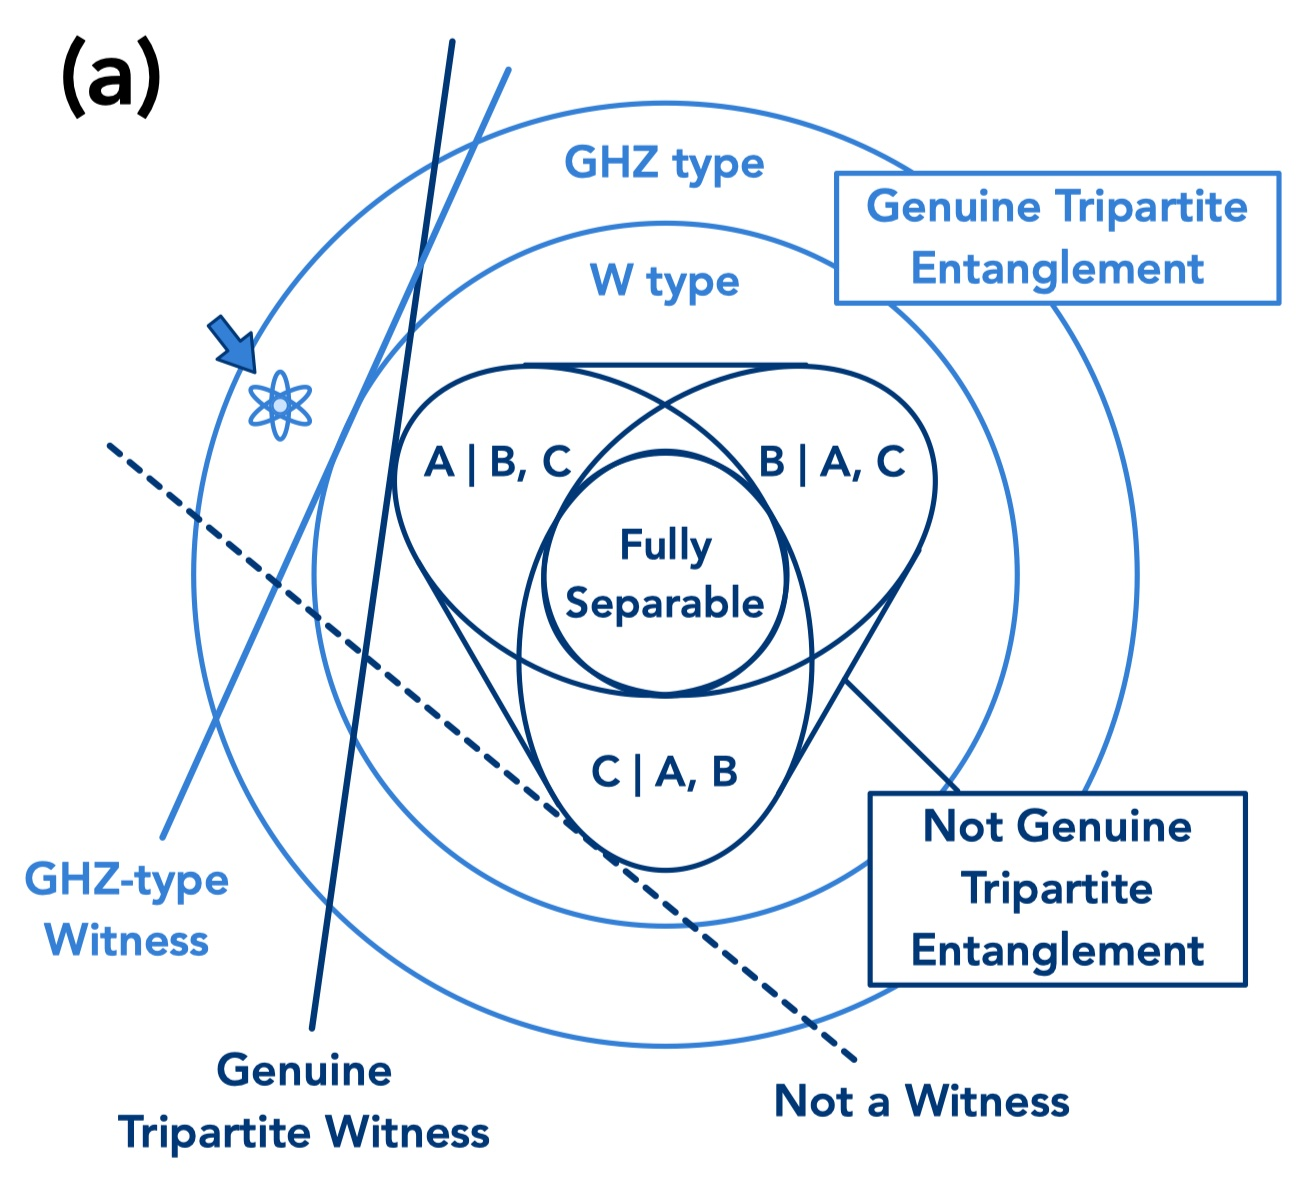
\includegraphics[width=.9\linewidth]{gme.jpg}
	% \end{subfigure}
	% \begin{subfigure}{0.6\textwidth}
		\centering
		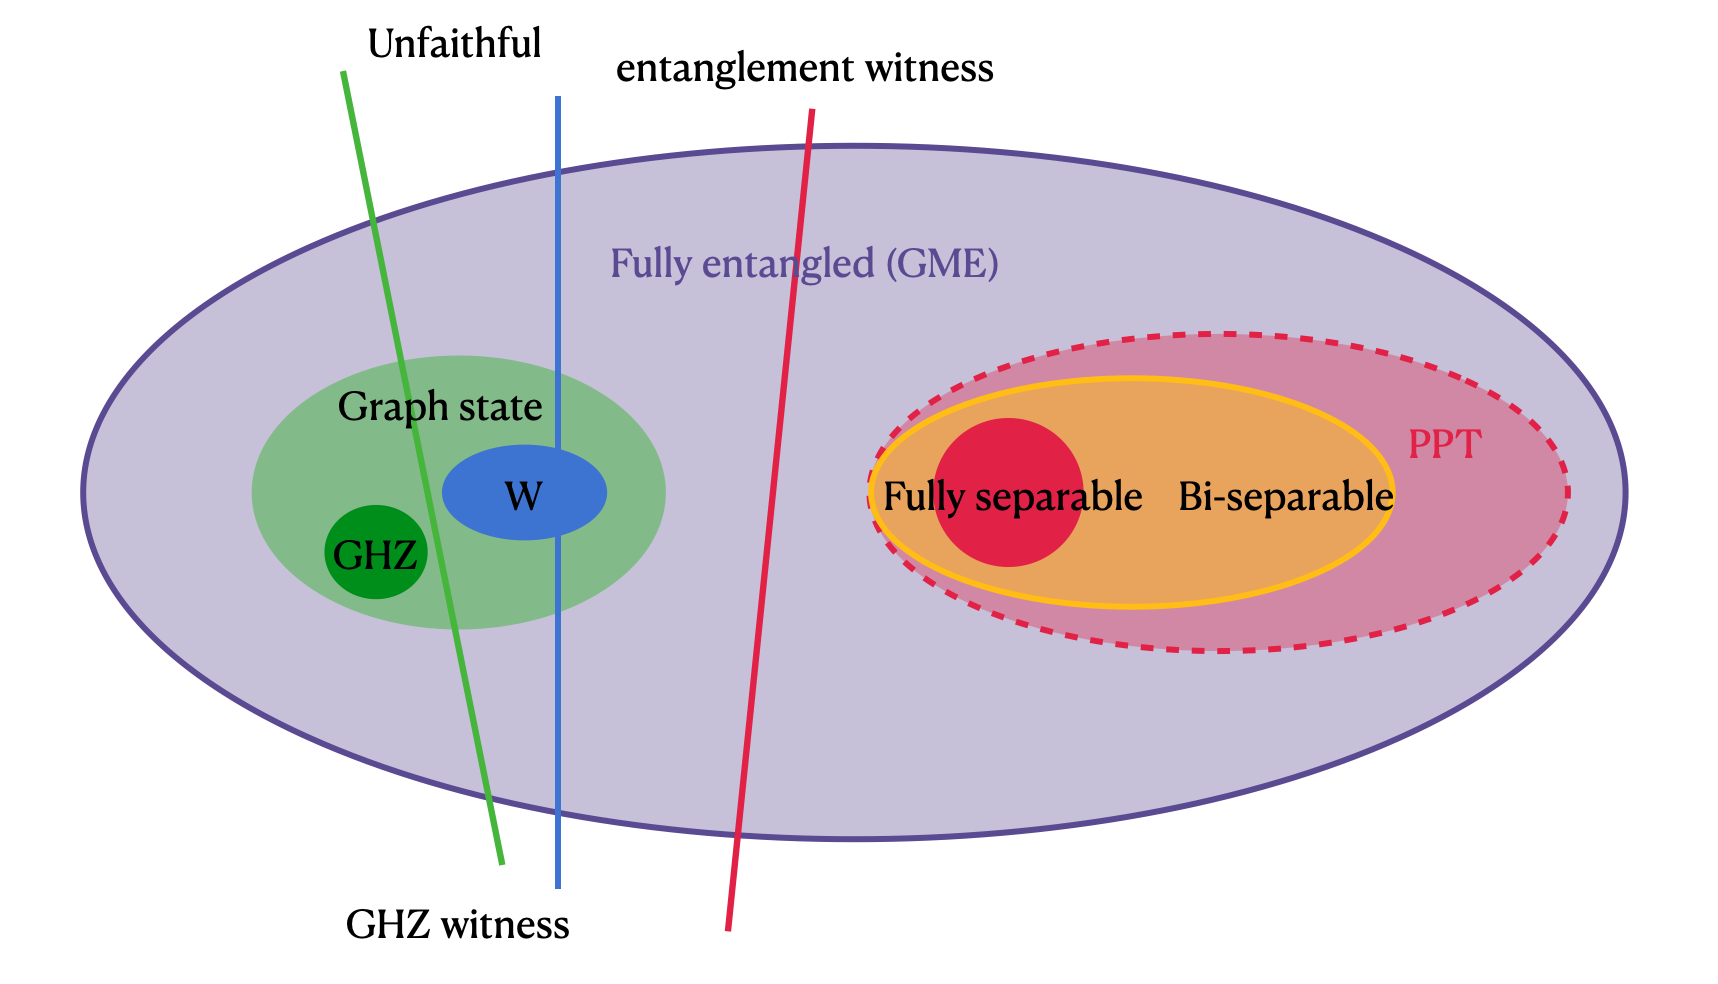
\includegraphics[width=.5\linewidth]{witness.png}
	% \end{subfigure}
	% \begin{subfigure}{0.3\textwidth}
	% 	\centering
	% 	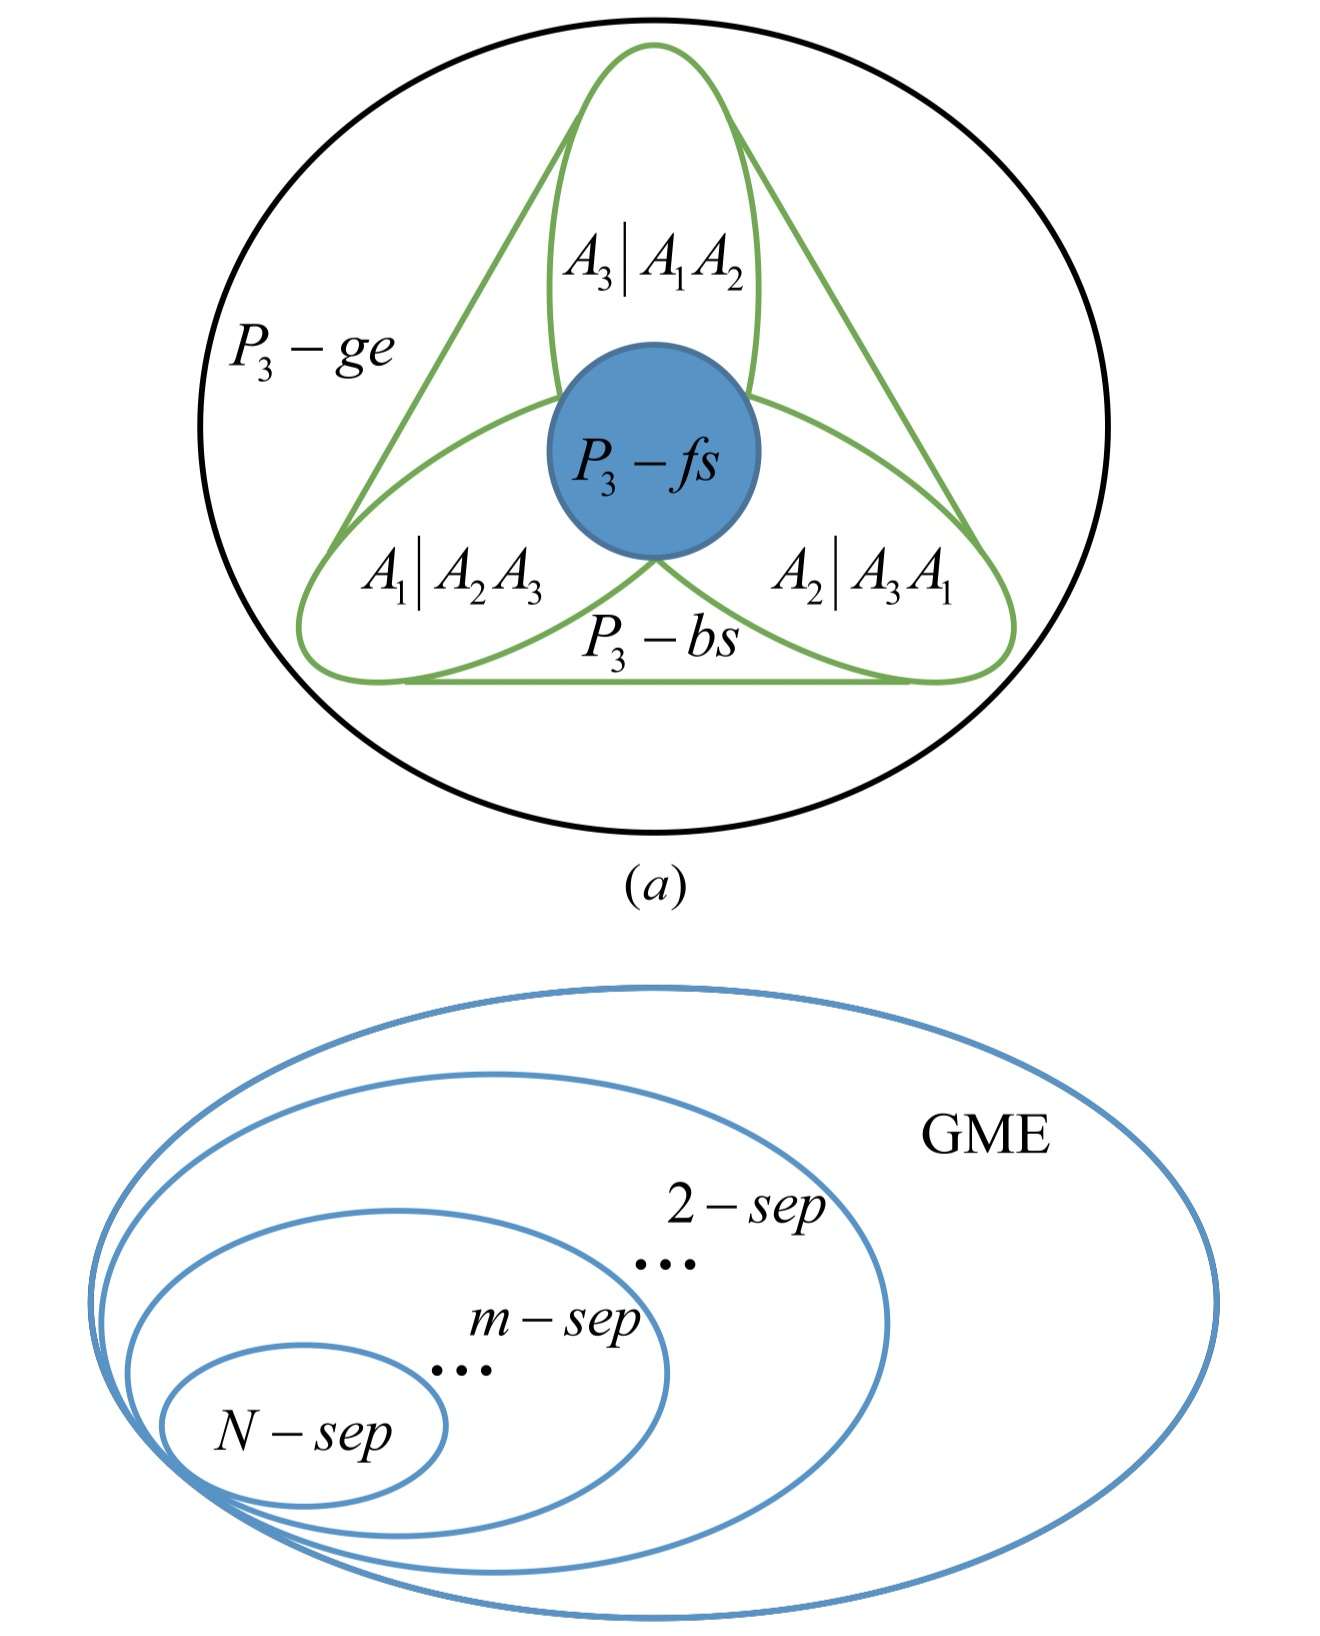
\includegraphics[width=.8\linewidth]{sep.jpg}
	% \end{subfigure}
	% \begin{subfigure}{0.35\textwidth}
	% 	\centering
	% 	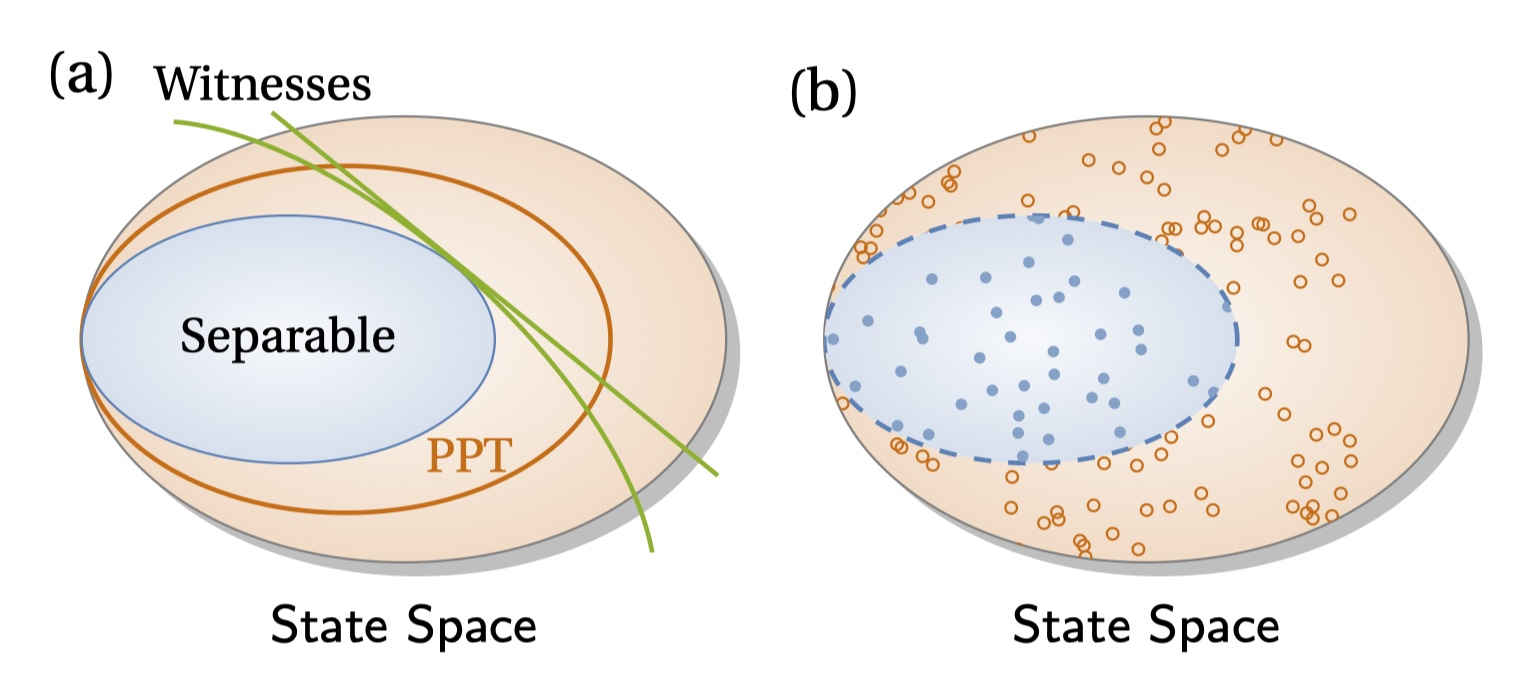
\includegraphics[width=.9\linewidth]{ppt.jpg}
	% \end{subfigure}
	\caption{(a) \nameref{def:entanglement_witness}, \nameref{thm:ppt}, \nameref{def:svm} (kernel)?. convex hull... The witness is depicted by the line in state space $\Tr(\dm\ew)=0$}
	\label{fig:entangle}
\end{figure}
% \begin{theorem}
% 	k local measurements. Here, k is the chromatic number (minimal \nameref{exm:colorable}) of the corresponding graph, typically, a small constant independent of the number of qubits.
% \end{theorem}

\subsubsection{Beyond fidelity and stabilizer witness (robustness)}
the authors coined the term faithful.


% \begin{remark}[universal entanglement witness]
	\cite{sciaraUniversalPartiteLevel2019}
	% Since the witness tests for a specif state, a successful measurement of the operator also provides information about the state structure and phase, rather than only confirming the presence of entanglement. 
	For example, a witness specifically designed for a four-qubit compact cluster state [16] confirms, when its expectation value is negative, the presence of that particular state having a very specific density function, while a positive measured expectation value of that operator only provides information that the tested state is not a compact cluster state. 
	Indeed, the same witness, if applied to a four-qubit linear cluster or GHZ [17] states, would result in a positive measured expectation value, even though these two states are both highly entangled [17, 18]. 
	% Bell’s theorem without inequalities, Am. J. Phys. 58, 1131 (1990).
	% G. Tóth and O. Gühne, Entanglement detection in the stabilizer formalism
	Hence, a witness is a threshold test that can only detect the presence of a specific state. 
	In contrast to an entanglement monotone (e.g. the entanglement entropy [6]), which determines the amount of entanglement, a witness cannot be used to quantify entanglement.	
% \end{remark}

Weilenmann et. al \cite{weilenmannEntanglementDetectionMeasuring2020} proposed the idea of unfaithful states which systematically analyze entangled state with noise cannot be detected by fidelity witness.
faithful states are useful for quantum teleportation.
This shows that fidelity-based entanglement witnesses detect entanglement that is useful.
\cite{guhneGeometryFaithfulEntanglement2021} 
the faithfulness of a twoqubit state, allowing for a physical interpretation of unfaithful two-qubit states as exactly those entangled states that are not useful for teleportation.
\cite{riccardiExploringRelationshipFaithfulness2021}
\cite{huOptimizedDetectionHighDimensional2021}
\begin{definition}[unfaithful state]\label{def:unfaithful_state}
\end{definition}
They found that for $d \ge 3$ that almost all states in the Hilbert space are unfaithful. 
For $d > 5$, the authors find that all states they generated are entangled but at the same time unfaithful, regardless of what metric is used to sample them.
Although there are nonlinear witnesses which also can detect entanglement in unfaithful states, they usually require more measurements [].
Moreover, they can only be applied to bipartite systems, which means they cannot be generalized to detect genuine entanglement in multipartite states.
Detecting Entanglement in Unfaithful States \cite{zhanDetectingEntanglementUnfaithful2021}.

For non-stabilizer case, \cite{zhangEfficientEntanglementGeneration2021} \cite{zhuMachineLearningDerivedEntanglement2021}
$C$ is hard to compute? non-stabilizer state? SWAP?
% \begin{question}
% \end{question}
% \begin{equation}\label{eq:noisy_state}
% 	\dm_{\noise}' = (1-p_{\noise}) \op{G} + p_{\noise} \frac{\identity}{2^n}
% \end{equation}
$p_{\noise}$ indicates the robustness of the algorithm (witness).
% \begin{remark}[\cite{zhouDetectingMultipartiteEntanglement2019}]
	the largest noise tolerance $p_{\text{limit}}$ just related to the \textbf{chromatic number} of the graph ($k$ local measurements) \cite{zhouDetectingMultipartiteEntanglement2019}.(\nameref{def:graph_property})
% \end{remark}
% \begin{question}
% 	how far white noise?
	other noise (depolarization)? e.g., flip error, phase error?, local, random unitary transformation?
	find optimal (robustness) entanglement witness by classical machine learning (quantum circuit?)
	tradeoff between (white noise) tolerance (robustness) and efficiency (number of measurements).
% \end{question}


\section{Classical-quantum hybrid, end-to-end detection protocol}


% \section{Classical, data-powered, and quantum algorithms}
In this paper, we focus on the entanglement structure dectection for graph states.
with training data
\begin{problem}[Learning entanglement witness with training data]
	\nameref{prm:separable}
	\begin{itemize}
		\item \textbf{Input}: specific entanglement structures $y$ and corresponding synthetic data (density matrices $\dm$) with labels $y$
		\item \textbf{Output}: find the classifier with high accuracy and minimal features $\vbx:=$
	\end{itemize}
\end{problem}
The idea is to feed the classifier by a large amount of sampled trial states
as well as their corresponding class labels.
% \begin{problem}[detect graph state entanglement structure?]
% 	problem with/without training data
% 	\begin{itemize}
% 		\item \textbf{Input}: a graph $\graph$ encoding in a graph state $\ket{\graph}$;
% 		adjacency matrix $A$?
% 		\item \textbf{Output}: entanglement structure: \textsf{\nameref{def:gme}}??
% 	\end{itemize}
% % with training data: 
% \end{problem}
% \begin{itemize}
% 	\item \textbf{features}: classical shadow?
% 	\item label: 
% \end{itemize}


\subsection{Estimate classical features of quantum states}
To make use of classical machine learning method, we need the classical \textbf{features} of quantum states.
We cannot directly process quantum data (raw data).
% \textbf{features}: classical shadow? raw data? quantum data, label: entangled?
In our pipeline, we focus on classical shadow.

\nameref{def:classical_shadow} \cite{huangPredictingManyProperties2020}: estimate entanglment witness (fixed but unknown target state, e.g., tripartite GHZ)
\textbf{Classical shadows (Clifford measurements) of logarithmic size allow for checking a large number of potential entanglement witnesses simultaneously}.
Directly measuring M different entanglement witnesses requires a number of quantum measurements that scales (at least) linearly in $M$. In contrast, classical shadows get by with $\log(M)$-many measurements only.
classical shadows are based on random Clifford measurements and do not depend on the structure of the concrete witness in question. In contrast, direct estimation crucially depends on the concrete witness in question and may be considerably more difficult to implement.

% \subsection{Tomography and trace estimation}
% \label{sec:shadow_tomography}
The brute force approach is to fully characterize a system by performing quantum state tomography and calculating separability measures from the recovered density matrix.
Intuitively, a general tomography \cite{altepeterPhotonicStateTomography2005} that extract (recover) all information of a state requires exponential copies (samples/measurements).
\begin{problem}[quantum state tomography]\label{prm:full_tomography}
	Informally, quantum state tomography refers to the task of estimating complete description (density matrix) of an unknown $N$-dimensional quantum mixed state $\dm$ within some error, 
	given the ability to prepare and measure $m$ copies $\dm^{\otimes m}$.
\end{problem}
% \begin{problem}[full tomography]\label{prm:full_tomography}
% 	In contrast to \nameref{prm:shadow_tomography}, we refer to \emph{full tomography} here
% 	\begin{itemize}
% 		\item \textbf{Input}: Given a \textbf{unknown} $N$-dimensional mixed state $\dm$
% 		\item \textbf{Output}: a complete description? of $\dm$ (decomposition coefficients) with error?
% 		Stokes parameter $S_i\equiv \Tr(\hat{\sigma}_i \dm)$
% 		\begin{equation}\label{eq:stokes_tomography}
% 			\dm = \frac{1}{2^n} \sum_{i_1,i_2,\dots,i_n=0}^3
% 			S_{i_1,i_2,\dots,i_n} 
% 			\hat{\sigma}_{i_1} \otimes \hat{\sigma}_{i_2} \otimes \dots \otimes \hat{\sigma}_{i_n} 
% 			,\;
% 			\bm{\sigma}\in \qty{\identity,\sx,\sy,\sz}^n
% 		\end{equation}
% 	\end{itemize}
% \end{problem}
However, tomography is experimentally and computationally demanding; for a state consisting of $n$ particles, with each residing in a $d$-dimensional Hilbert space, we would have to perform $M = \bigO(d^{2n})$ measurements.
\begin{theorem}[lower bound of \nameref{prm:full_tomography}?\cite{haahSampleoptimalTomographyQuantum2017}]
	Known fundamental lower bounds [66, 73] state that classical shadows of exponential size (at least) $T = \Omega( 2^n / \epsilon^2)$ are required to $\epsilon$-approximate $\dm$ in trace \nameref{def:distance}.
\end{theorem}
% \begin{problem}[Fidelity estimate]
% 	defined as follows
% 	\begin{itemize}
% 		\item \textbf{Input}: Given two density matrices $\dm$ and $\dm'$, 
% 		\item \textbf{Output}: \nameref{def:fidelity} with error $\epsilon$
% 	\end{itemize}
% \end{problem}
In quantum mechanics, interesting properties are often linear functions of the underlying density matrix $\dm$.
For example, the fidelity with a pure target state, entanglement witnesses fit this framework.
\begin{problem}[trace estimation]\label{prm:trace_estimation}
	related problems defined as follows
	\begin{itemize}
		\item \textbf{Input}: Given an observable (Hermitian) $\ob$ and (copies of) a mixed state $\dm$ or several states ($\dm',\dots,\dm_m$), 
		\item \textbf{Output}: 
		with error $\epsilon$ measured by trace \nameref{def:distance} (\nameref{def:fidelity}...), to estimate
		linear functions (mostly): the expectation value $\expval{\ob}=\Tr(\ob \dm) $, entanglement witness, tomography; 
		nonlinear functions: \nameref{def:entropy};
		multivariate functions:  $\Tr(\dm_1 \cdots \dm_m)$, \nameref{def:quantum_kernel} $\Tr(\dm\dm')$,  quadratic $\Tr(\ob \dm_i \otimes \dm_j)$, \nameref{def:fidelity} $F(\dm,\dm')$, \nameref{def:distance}??;
	\end{itemize}
\end{problem}

Nevertheless, we usually only need specific properties of a target state rather than full classical descriptions about the state.
This enables the possibility to shadow tomography.
\begin{problem}[shadow tomography]\label{prm:shadow_tomography}
	\emph{shadow tomography}
	\begin{itemize}
		\item \textbf{Input}: an \textbf{unknown} $N$-dimensional mixed state $\rho$, $M$ known 2-outcome measurements $E_1,\dots,E_M$
		\item \textbf{Output}: estimate $\probability[E_i \text{ accept } \dm]$ to within additive error $\epsilon$, $\forall i\in [M]$, with $\ge 2/3$ success probability.	
	\end{itemize}
\end{problem}
\begin{theorem}[bounds of shadow tomography \cite{aaronsonShadowTomographyQuantum2018}]\label{thm:shadow_tomography}
	It is possible to do \nameref{prm:shadow_tomography} using $\tilde{\bigO}(\frac{\log^4 M\cdot \log N}{\epsilon^4})$ copies. [no construction algorithm?]
	sample complexity lower bound $\Omega(\log (M) \cdot \epsilon^{-2})$, 
\end{theorem}
% more details in \cref{sec:classical_shadow}
\begin{remark}[compare shadow tomography with classical shadow \cite{huangPredictingManyProperties2020}]
	While very efficient in terms of samples, Aaronson's procedure is very demanding in terms of quantum hardware - a concrete implementation of the proposed protocol requires \textbf{exponentially long quantum circuits} that act collectively on all the copies of the unknown state stored in a quantum memory.
	% [compare shadow tomography and classical shadow ??]
\end{remark}


\subsubsection{Classical shadow and derandomized version}\label{sec:classical_shadow}
Inspired by Aaronson's shadow tomography \cite{aaronsonShadowTomographyQuantum2018}, Huang et. al \cite{huangPredictingManyProperties2020} introduce classical shadow.
A classical shadow is a succinct classical description of a quantum state, which can be extracted by performing reasonably simple single-copy measurements on a reasonably small number of copies of the state.
The classical shadow attempts to approximate this expectation value by an empirical average over $T$ independent samples, much like Monte Carlo sampling approximates an integral.
\begin{definition}[classical shadow]\label{def:classical_shadow}
	classical shadow (snapshots) $\dm_{cs}$
	\begin{equation}
		\dm_{cs} = \mathcal{M}^{-1} \qty(U^\dagger \op{\hat{b}} U)
	\end{equation}
	such that we can predict the linear function with classical shadows
	\begin{equation}
		o_i = \Tr(O_i \dm_{cs})
		\text{ obeys }
		\expectation[o] =\Tr(O_i \dm)
	\end{equation}
\end{definition}
% \begin{remark}
The classical shadow size required to accurately approximate all reduced $r$-body density matrices scales exponentially in subsystem size $r$, but is independent of the total number of qubits $n$.
% \end{remark}

% \begin{algorithm}[H]
%     \DontPrintSemicolon
%     \SetKwInOut{Input}{input}
%     \SetKwInOut{Output}{output}
%     \Input{(copies of) density matrix $\dm$, an entanglement witness (observable) $\ew$}
%     \Output{$\Tr(P_x \dm ), \forall x \in \qty{ I, X, Y, Z }^n$}
%     \BlankLine
%     % \For{ $i = 1,2, \ldots, m$} {
%     %     $P_x$  \tcp*{estimate entanglement witness by quantum ML}
%     %     % \tcc{comment in a new line}
%     % % {\Return $\Tr(\ew\dm)$ }
%     % }
%     \Return estimation of $\Tr(\ew\dm)$ 
%     % \Return entangled ? GME ? separable with certain partition?
%     \caption{features for \nameref{def:entanglement_witness}}
%     \label{alg:entanglement_witness}
% \end{algorithm}
\begin{algorithm}[H]
    \DontPrintSemicolon
    \SetKwInOut{Input}{input}
    \SetKwInOut{Output}{output}
    \Input{an (unknown) density matrix $\dm$ (many copies, black-box access to a circuit preparing a state), an entanglement witness (observable) $\ew$}
	% , observables $\ob$...
    \Output{\nameref{def:classical_shadow} $\dm_{cs}$,$\Tr(P_x \dm ), \forall x \in \qty{ I, X, Y, Z }^n$}
    \BlankLine
    \For{ $i = 1,2, \ldots, N$} {
        $\dm\mapsto \U\dm \U^\dagger$ \tcp*{apply a random unitary to rotate the state}
		$\mapsto \ket{b}$... \tcp*{perform a computational-basis measurement}
		$\dm_{cs}=\mathcal{M}^{-1}\qty(\U^\dagger \op{b} \U)$ \tcp*{measurement outcome $\ket{b}\in \qty{0,1}^n $, $\mathcal{M}$ quantum channel}
        % \tcc{comment in a new line}
    % {\Return ?}
    }
    \Return $S(\dm,N)=\qty{\dm_{cs_1}=\mathcal{M}^{-1}\qty(\U_1^\dagger\op{b_1}\U_1),\dots,\dm_{cs_N}}$ \tcp*{call this array the classical shadow of $\dm$}
	\tcc{estimate features}
	\Return estimation of $\Tr(\ew\dm)$ 
    \caption{Classical Shadow (tomography): features for \nameref{def:entanglement_witness}}
    \label{alg:classical_shadow}
\end{algorithm}
A classical shadow is created by repeatedly performing a simple procedure: Apply a unitary transformation $\dm \mapsto \U \dm \U^\dagger$, and then measure all the qubits in the computational basis. The number of times this procedure is repeated is called the size of the classical shadow. The transformation $U$ is randomly selected from an ensemble of unitaries, and different ensembles lead to different versions of the procedure that have characteristic strengths and weaknesses.
Classical shadows with size of order $\log(M)$ suffice to predict $M$ target functions $\qty{\ob_1,\dots,\ob_M}$.
% \begin{lemma}
% 	predict linear function with shadow shadow:
% 	the variance
% 	\begin{equation}
% 		\variance[o] = \expectation[(o-\expectation[o])^2]
% 		\le \norm{O - \frac{\Tr(O)}{2^n} \identity}^2_{\shadow}
% 	\end{equation}
% \end{lemma}
% \begin{theorem}\label{thm:classical_shadow_upper}
% 	Fix a measurement primitive $\mathcal{U}$??, a collection $\qty{\ob_1,\dots,\ob_M}$ of $2^n\times 2^n$ Hermitian matrices and accuracy parameters $\epsilon,\delta\in[0,1]$.
% 	Set 
% 	\begin{equation}
% 		K = 2\log (2M/\delta)
% 		,\quad
% 		N = \frac{34}{\epsilon^2}\max_{1\le i\le M} \norm{\ob_i-\frac{\Tr(O_i)}{2^n} \identity}^2_{\shadow}
% 	\end{equation}
% 	where $\norm{\cdot}_{\shadow}$ is \nameref{def:shadow_norm}. 
% 	Then, a collection of NK independent classical shadows allow for accurately predicting all features via median of means prediction
% 	\begin{equation}
% 		\abs{o_i (N,K), -\Tr(O_i \dm)}\le \epsilon,\; \forall i\le i \le M
% 	\end{equation}
% 	wieth probability at least $1-\delta$.
% 	$o_i(N,K)=\textup{median}\qty{\Tr(\ob_i\dm_{(1)}),\dots,\Tr(\ob_i\dm_{(K)})}$
% 	% sample complexity
% 	% \begin{equation}
% 	% 	N_{tot} = \bigO \qty(
% 	% 		\frac{\log (M)}{\epsilon^2} \max_{1\le i\le M} 
% 	% 		\norm{O_i - \frac{\Tr(O_i)}{2^n} \identity}^2_{\shadow}
% 	% 	)
% 	% \end{equation}
% \end{theorem}
% \begin{definition}[shadow norm]\label{def:shadow_norm}
% 	$\norm{\cdot}_{\shadow}$ is shadow norm that only depends on the measurement primitive:
% 	\begin{equation}
% 		\norm{O}_{\shadow} =\max_{\sigma:state} \qty(
% 			\expectation_{U\sim \mathcal{U}}
% 			\sum_{b\in \qty{0,1}^n } \mel{b}{\U\sigma\U^\dagger}{b} 
% 			\mel{b}{\U\mathcal{M}^{-1}(O) \U^\dagger}{b}^2 
% 		)^{1/2}
% 	\end{equation}
% 	(nonnegative, homogeneous, triangle inequality)
% \end{definition}

\begin{theorem}[Pauli/Clifford measurements]\label{thm:classical_shadow_lower}
	Any procedure based ona fixed set of single-copy local measurements that can predict,
	with additive error $\epsilon$, $M$ arbitrary $k$-local linear function $\Tr(\ob_i\dm)$,
	requires at least (lower bound)
	$\Omega(\log(M) 3^k/\epsilon^2)$ copies of the state $\dm$.
	$\Omega(\log(M) \max_i\Tr(\ob_i^2)/\epsilon^2)$ 
\end{theorem}
% Consider a simple family of entanglement witnesses with compatible structure:  (ansatz??)
% \begin{equation}
% 	O:= O(V_A,V_B,V_C)=V_A\otimes V_B \otimes V_C \op{\psi_{\ghz}^+} V_A^\dagger\otimes V_B^\dagger \otimes V_C^\dagger
% \end{equation}
% the single-qubit unitaries $V_A,V_B,V_C$ parametrize differenet witnesses.


% \subsubsection{Derandomization}
Derandomization can and should be viewed as a refinement of the original classical shadows idea. \cite{huangEfficientEstimationPauli2021} \cite{elbenMixedstateEntanglementLocal2020}

\subsubsection{Estimate expectation by (classical/quantum) machine learning}
% \subsubsection{training data and classical kernel methods}
\cite{huangProvablyEfficientMachine2021}
$\sigma_T(\dm(x_l))$ is the classical shadow representation of $\dm(x_l)$, 
a $2^n\times 2^n$ matrix that reproduces $\dm(x_l)$ in expectation over random Pauli measurements.
\begin{equation}
	\qty{x_l\to\sigma_T(\dm(x_l))}_{l=1}^N
\end{equation}
\begin{definition}[shadow kernel]\label{def:shadow_kernel}
	given two density matrices (quantum states) $\rho$ and $\rho'$,
	\emph{shadow kernel} \cite{huangPredictingManyProperties2020} is 
	\begin{equation}
		k_{\shadow}(S_T(\dm),S_T'(\dm')) := 
		\exp( \frac{\tau}{T^2}
			\sum_{t,t'=1}^{T} \exp( \frac{\gamma}{n} 
			\sum_{i=1}^n \Tr(\sigma_i^{(t)}\sigma_i^{(t')}) ) 
			)
	\end{equation}	
	where $S_T(\dm)$ is the classical shadow representation of $\dm$.
	The computation time for the inner product is $\bigO(nT^2)$,
	linear in the system size $n$ and quadratic in $T$,
	the number of copies of each quantum state which are measured to construct the classical shadow.
\end{definition}
% \begin{figure}[!ht]
% 	\centering
% 	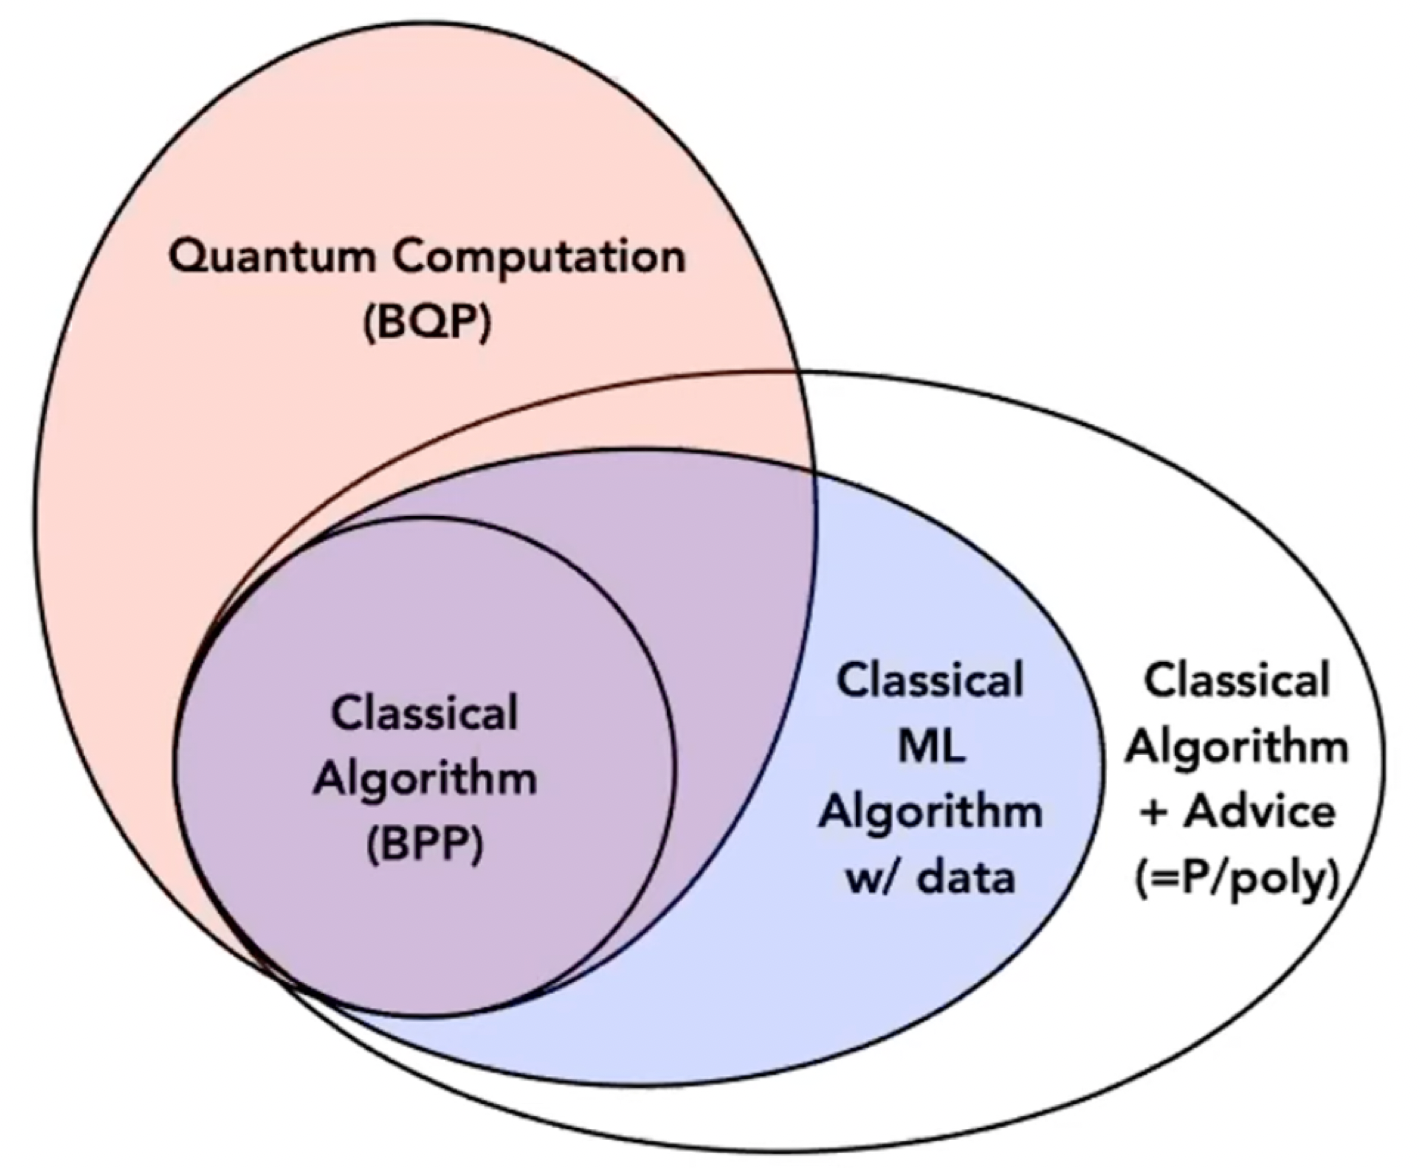
\includegraphics[scale=.2]{data.png}
% 	% 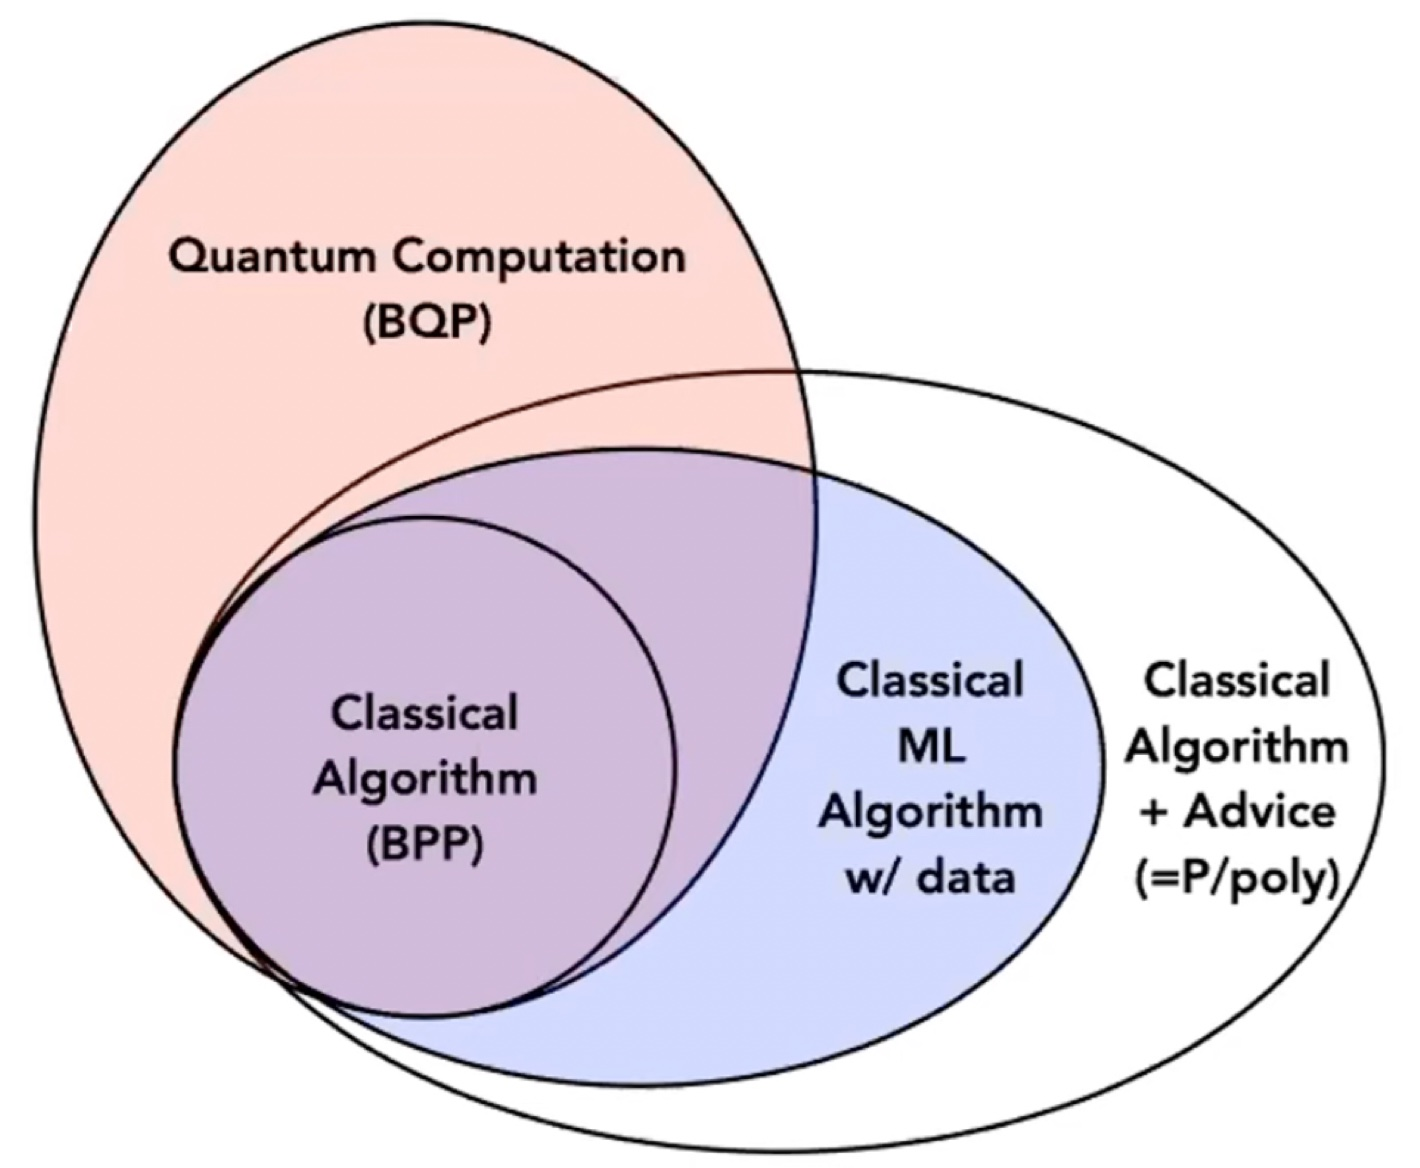
\includegraphics[width=.35\linewidth]{data.jpg}
% 	\caption{computational model powered by training data}
% \end{figure}

\begin{proposition}[\cite{huangPowerDataQuantum2021}]
	exist quantum advantage in machine learning (not significant, practical)	...
	discrete log, factoring...
\end{proposition}
% \begin{theorem}[informal \cite{huangPowerDataQuantum2021}]
% 	data learning
% 	\begin{itemize}
% 		\item machine learning (strictly) more powerful than BPP
% 		\item exist quantum advantage in machine learning (not significant, practical)
% 	\end{itemize}
% \end{theorem}

% \subsubsection{Estimate entanglement witness by (quantum) machine learning}
though, that while there is no large advantage in query complexity, a substantial quantum advantage in computational complexity is possible.

The quantum ML algorithm accesses the quantum channel $\mathcal{E}_\dm$ multiple times to obtain multiple copies of the underlying quantum state $\dm$. Each access to $\mathcal{E}_\dm$ allows us to obtain one copy of $\dm$. Then, the quantum ML algorithm performs a sequence of measurements on the copies of $\dm$ to accurately predict $\Tr(P_x \dm ), \forall x \in \qty{ I, X, Y, Z }^n$.

\begin{theorem}[\cite{huangInformationtheoreticBoundsQuantum2021}]\label{thm:quantum_ml_estimate_bound}
	For $M$ Pauli opertors, there is a (quantum) procedure estimate every expectation value $\Tr(P_x \dm),\forall i=1,\dots,M$ within error $\epsilon$ under probability at least $1-\delta $ by performing POVM measurements on $\bigO(\log(M/\delta)\epsilon^{-4})$ copies of the unknown quantum state $\dm$.
	($M=4^n$ implies linear copy for full tomography???)
% \end{theorem}
% \begin{theorem}[\cite{huangInformationtheoreticBoundsQuantum2021}]\label{thm:quantum_vs_classical}
	We rigorously show that, for any quantum process $\mathcal{E}$, observables $\ob$, and distribution $\mathcal{D}$, and for any quantum ML model, one can always design a classical ML model achieving a similar average prediction error such that $N_C$ (number of experiments?) is larger than $N_Q$ by at worst a small polynomial factor.

	In contrast, for achieving accurate prediction on all inputs, we prove that \textbf{exponential quantum advantage is possible}. For example, to predict expectations of all \textbf{Pauli observables} (entanglement witness??) in an $n$-qubit system $\dm$, classical ML models require $2^{\Omega(n)}$ copies of $\dm$ , but we present a quantum ML model using only $\bigO(n)$ copies.
\end{theorem}
\cite{huangPredictingManyProperties2020}
\cite{huangInformationtheoreticBoundsQuantum2021}
\cite{huangPowerDataQuantum2021}
\cite{aaronsonShadowTomographyQuantum2018}
\begin{table}[!ht]
	\centering
	\begin{tabular}{c|c|c}
		& circuits & number of copies (measurements) \\
		\hline
		\nameref{prm:shadow_tomography} & exp circuit? & \cref{thm:shadow_tomography} \\  
		\nameref{def:classical_shadow} & & \\
		derandomized & & better performance \\  
		% quantum circuit  &  \cref{thm:multivariate_trace} (c-depth?) & ? \\  
		quantum/classical ML  & & Q. advantage 
		% \cref{thm:quantum_vs_classical} 
		\cref{thm:quantum_ml_estimate_bound} \\  
		\hline
	\end{tabular}
	\caption{complexity (measures) of different trace estimation methods}
\end{table}

generative neural network \cite{zhuFlexibleLearningQuantum2022}
	
% \subsection{Quantum trace (kernel) estimation by quantum circuits}



% \subsubsection{Variational quantum kernel estimation (hybrid)}

\subsection{Training a witness for certain entanglement with SVM}


% \subsubsection{Related works}
% \begin{itemize}
% \item 
separability classifier by classical neural network \cite{luSeparabilityEntanglementClassifierMachine2018}:
input: sythetic random density matrices;
output: a classical classifier for \nameref{def:bipartite_separable} (independent of state??).
 (feature: synthetic density matrix with noise flatten as a real vector $\vbx\in\realnumber^{d_A^2d_B^2-1}$)  (label: separable or entangled by \nameref{thm:ppt}, CHA), and then train the classifier to predict the class labels of new states that it has not encountered before.
Previous methods \textbf{only detect a limited part of the state space}, e.g. different entangled states often require different \nameref{def:entanglement_witness}. In contrast, this classifier can handle a variety?? of input states once properly trained \cref{fig:entangle}.
% \item 
Bell inequlaity and NN \cite{maTransformingBellInequalities2018}. 
a linear Bell-like predictor by generalizing the CHSH operator $\ew_{\text{ml}}:=\vb{P}\cdot\vb{w}_{\text{ml}}$ in \cref{eq:chsh} where the coefficients (or weights) $\vb{w}$ are determined by machine learning.
tomographic ansatz better performance.
% However, the challenge is to find a reliable way for labelling the quantum states in the training set.
% Overall, for scaling up this method for detecting higher-dimensional quantum entanglement, the major challenge is related to a lack of reliable method for labeling the entanglement.
% We have constructed such a universal state classifier for a pair of qubits; we find that the performance depends heavily on the testing sets; the major source of error comes from the data near the boundary between entangled and separable states.
% Tomographic predictors make use of all information of a given quantum state and is used to benchmark the performance of Belllike predictors, which employs a subset of non-orthogonal measurements setting.
% \begin{remark}
% \cite{luSeparabilityEntanglementClassifierMachine2018} reported that they independently combined machine learning and semidefinite programming to train their predictors as quantum state classifiers. Using all information without any prior knowledge, the error of their predictor is always around 10\% on general 2-qubit system. However, our tomographic predictor performs below 2\% on the same ensembles with 3000 hidden neurons.
% \end{remark}
training a universal classifier for multi-qubit, high-dimensional system is hard (boundary).
it is difficult to generate general GME states or label general states.
Tomography is necessary for universal entanglement detection with single-copy observables (non-adaptive schemes) \cite{luTomographyNecessaryUniversal2016}
% \item 

% \item 
classical SVM: 
This method the ability to obtain witnesses that require only local measurements even when the target state is a \textbf{non-stabilizer state} $W$ state (normally need nonlocal measurements).
feature: $\vbx_{\vec{k}}$ expectation of Pauli strings.
the training of an SVM is convex; if a solution exists for the given target state and ansatz, the optimal SVM will be found.
this SVM formalism allows for the programmatic removal of features, i.e., reducing the number of experimental measurements, in exchange for a lower tolerance to white noise, in a manner similar to [??].
% \item 
SVM, (universal), 4 qubit \cite{vintskevichClassificationFourqubitEntangled2022}
% \item 
% \end{itemize}

% \subsubsection{Our witness ansatz and optimization}
classical machine learning (SVM, NN) with \nameref{def:classical_shadow} \cite{huangProvablyEfficientMachine2021}??: classify phase, predict ground state, entanglement?
% \subsection{Variational (hybrid) quantum algorithms}
The quantum extension of this problem (classficiation/pattern recognition) is to replace the data points $\vbx_i$ with density matrices of quantum states $\dm_i$. 
Specifically, a quantum state classifier outputs a “label” associated with the state, for example, $\entangled$ or ``unentangled".
In actual experiments, we don't know entries of a density matrix.
Instead, we need measurements or \nameref{def:classical_shadow} as features of machine learning algorithms.


\begin{table}[!ht]
	\centering
	\begin{tabular}{c|c|c|c}
		& \# observables & weights & input state \\
		\hline
		% entanglement witness & & & known \\  
		\nameref{def:entanglement_witness} & constant? few local & fixed & known  \\  
		% convex?\cite{chakrabartiQuantumAlgorithmsLower2020} 
		Bell (CHSH) inequality & constant & fixed & unknown \\  
		% entangle spectrum \cite{horodeckiDirectDetectionQuantum2002} & & & unknown \\  
		tomographic witness & $4^n$ & trained & unknown \\  
		ML & ?? & trained & partially known \\  
		\hline
	\end{tabular}
	\caption{ansatz}
\end{table}
% \subsubsection{Variational entanglement witness (ansatz)}
an ansatz for \nameref{def:entanglement_witness} \cite{zhuMachineLearningDerivedEntanglement2021} (graph state entanglement)
\begin{equation}
	\ew_{\ansatz} := 
	% \sum_{k_1,k_2,\dots,k_n}  w_{k_1,k_2,\dots,k_n} \bigotimes_i^n \hat{\sigma}^{(k_i)}
	% ,\quad \hat{\sigma} \in \qty{\sx,\sy,\sz,\identity_{2\times 2}}
	\sum_{\vb{p}\in \qty{I,X,Y,Z}^n} w_{\vb{p}}  
	\bigotimes_i^n 
	% \hat{\sigma}^{(\vb{p}_i)}
	\vb{p}_i
\end{equation}
c.f. \nameref{prm:full_tomography} (Stokes parameters) \cref{eq:stokes_tomography}.
An SVM allows for the construction of a hyperplane $\expval{\ew}=\sum_k w_k \vbx_{k}$ that clearly delineates between separable states and the target entangled state (bipartite and \textbf{tripartite qubit and qudit}); this hyperplane is a \textbf{weighted sum of observables (`features') whose coefficients are optimized during the training of the SVM}.

We focus on kernel methods, as they not only provide provable guarantees, but are also very flexible in the functions they can learn. For example, recent advancements in theoretical machine learning show that training neural networks with large hidden layers is equivalent to training an ML model with a particular kernel, known as the neural tangent kernel \cite{jacotNeuralTangentKernel2020}.

\begin{algorithm}[H]
    \DontPrintSemicolon
    \SetKwInOut{Input}{input}
    \SetKwInOut{Output}{output}
    \Input{an entanglement witness (observable) ansatz $\ew_{\ml}=\vb{w}\cdot \vec{\sigma}$;\nameref{def:classical_shadow}? (features) with label (training data)}
    \Output{classifier $\vb{w}$; entanglement structure? decision \textsf{separble}; classify phase}
    \BlankLine
	\tcp*{---------------------------------------------- training phase ------------------------------------------------}
    \For{ $i = 1,2, \ldots, m$} {
        kernel estimation \tcp*{classical kernel}
        SVM \tcp*{SVM}
        % \tcc{comment in a new line}
    {\Return parameters $\vb{w}$ (SVM hyperplane)} \tcp*{parameters of the separating hyperplane in the feature space}
    }
	\tcp*{call classical shadow to extract features from quantum states}
	% \tcp*{============================================= prediction =============================================== //}
    \Return $ \vb{w}\cdot \vec{\sigma}<0 $: \textsf{separable} 
	\tcc{predict}
	\tcp*{============================================= testing phase =============================================== //}
    \caption{ansatz + classical shadow (..) + Classical learning (\nameref{def:svm}) }
    \label{alg:classical_learning}
\end{algorithm}

% \subsubsection{Variational trace estimate (direct)}
\begin{theorem}
	On quantum computers, evaluating the trace distances is probably hard since even judging whether $\dm$ and $\dm'$ have large or small trace distance is known to be QSZK-complete \cite{watrousQuantumComputationalComplexity2008}, where QSZK (quantum statistical zero-knowledge) is a complexity class that includes BQP (bounded-error quantum polynomial time).
	% Variational Quantum Algorithms for Trace Distance and Fidelity Estimation
\cite{chenVariationalQuantumAlgorithms2022}
\end{theorem}

% \subsection{Theoretic upper bounds and lower bounds}
% \cite{huangPredictingManyProperties2020}
% \cite{huangInformationtheoreticBoundsQuantum2021}
% \cite{huangPowerDataQuantum2021}
% \cite{aaronsonShadowTomographyQuantum2018}
% \cite{liuRigorousRobustQuantum2021}

% \begin{table}[!ht]
% \centering
% \begin{tabular}{c|c|c|c|c}
% 	& gate/depth/computation & measurements/samples & query? & input/unknown? \\  
% 	% necessary?sufficient
% 	\hline
% 	% \nameref{prm:full_tomography} & & N/A & $\bigO$, Holevo bound $\Omega$ & \\  
% 	\nameref{prm:shadow_tomography} & exp circuit? & \cref{thm:shadow_tomography} & N/A & unknown \\  
% 	% indirect? direct (no prior), promise & & & & \\  
% 	% promise (low-rank?), partial, decision? & & & & \\  
% 	\nameref{def:entanglement_witness} & N/A &  \cref{thm:entanglement_witness_gme} (constant?) & convex?\cite{chakrabartiQuantumAlgorithmsLower2020} & known \\  
% 	\nameref{def:classical_shadow}  & N/A & \cref{thm:classical_shadow_upper,thm:classical_shadow_lower} & N/A & unknown? \\  
% 	C. ML + C. \nameref{def:entanglement_witness} ansatz  & ?? & Q. advantage \cref{thm:quantum_vs_classical} & N/A & unknown \\  
% 	QML. \nameref{def:entanglement_witness} ansatz  & ?? & \cref{thm:quantum_ml_estimate_bound} & N/A & unknown \\  
% 	Q. \nameref{def:entanglement_spectroscopy} &  \cref{thm:multivariate_trace} (c-depth?) & & property test \cite{montanaroSurveyQuantumProperty2018} & unknown\\  
% 	% SVM + quantum kernel estimation &  & &  & ??\\  
% 	\hline
% \end{tabular}
% \caption{complexity (different measures) of different methods}
% \end{table}


% \begin{table}[!ht]
% 	\centering
% 	\begin{tabular}{c|c|c}
% 		& accuracy & complexity \\
% 		\hline
% 		linear SVM & & \\  
% 		kernel SVM & & \\  
% 		Neural network & & \\  
% 		neural kernel & & \\  
% 		quantum kernel & & \\  
% 		\hline
% 	\end{tabular}
% 	\caption{machine learning methods}
% \end{table}

% \subsubsection{Separations (complexity)}
% contrived problem (engineered dataset)? for exponential speedup

% \subsubsection{Obstacles (practical)}

% quantum advantages:
% \begin{itemize}
% 	\item no input encoding problem? \cite{tangQuantumPrincipalComponent2021} in most quantum machine learning algorithm.
% 	\item contrived problem (engineered dataset)? for exponential speedup
% 	% \item convex body query? complexity
% \end{itemize}
% obstacles: (i)

\section{Numerical simulation}
\subsection{Data preparation and state generation}
multi-partite entangled state: generate synthetic (engineered) data from (random graph?).
separable state from randomly ...
% \begin{figure}[!ht]
% 	\centering
% 	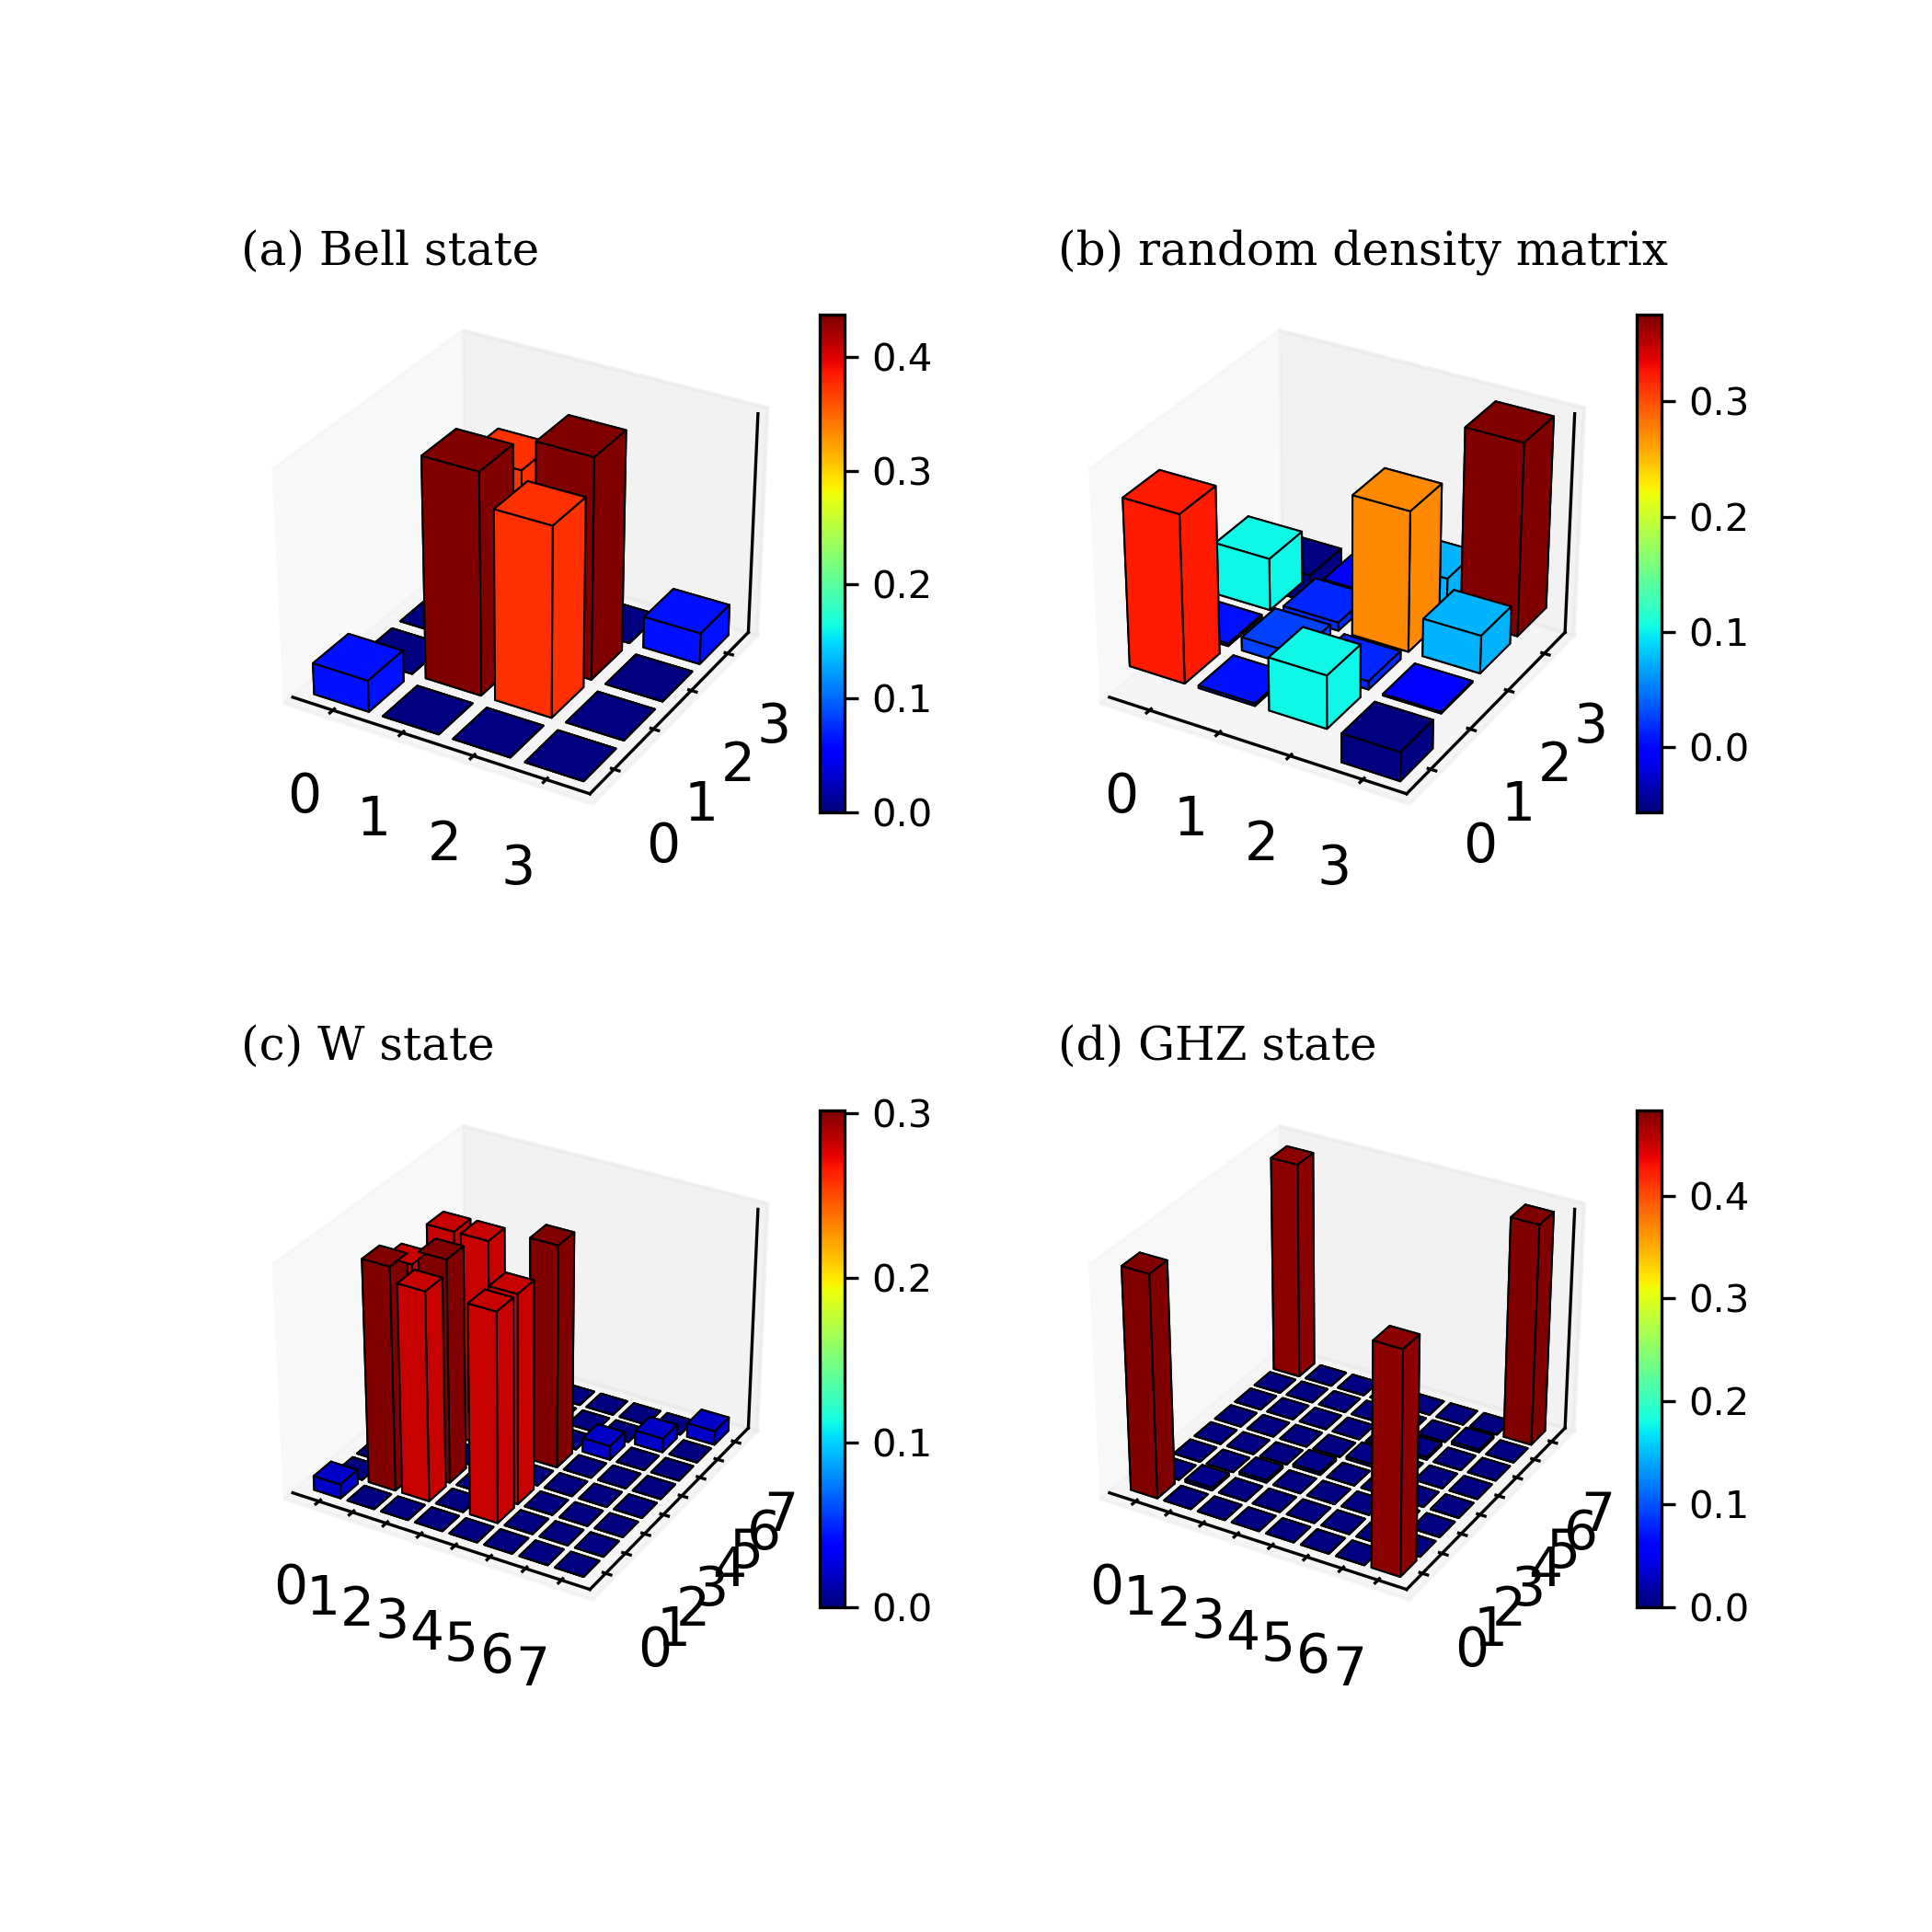
\includegraphics[width=.5\linewidth]{./notebook/dataset_sample.png}
% 	\caption{(a) three-qubit W state, (b) GHZ state with white noise}
% \end{figure}
\begin{figure}[!ht]
	\centering
	\begin{subfigure}{0.42\textwidth}
	\centering
		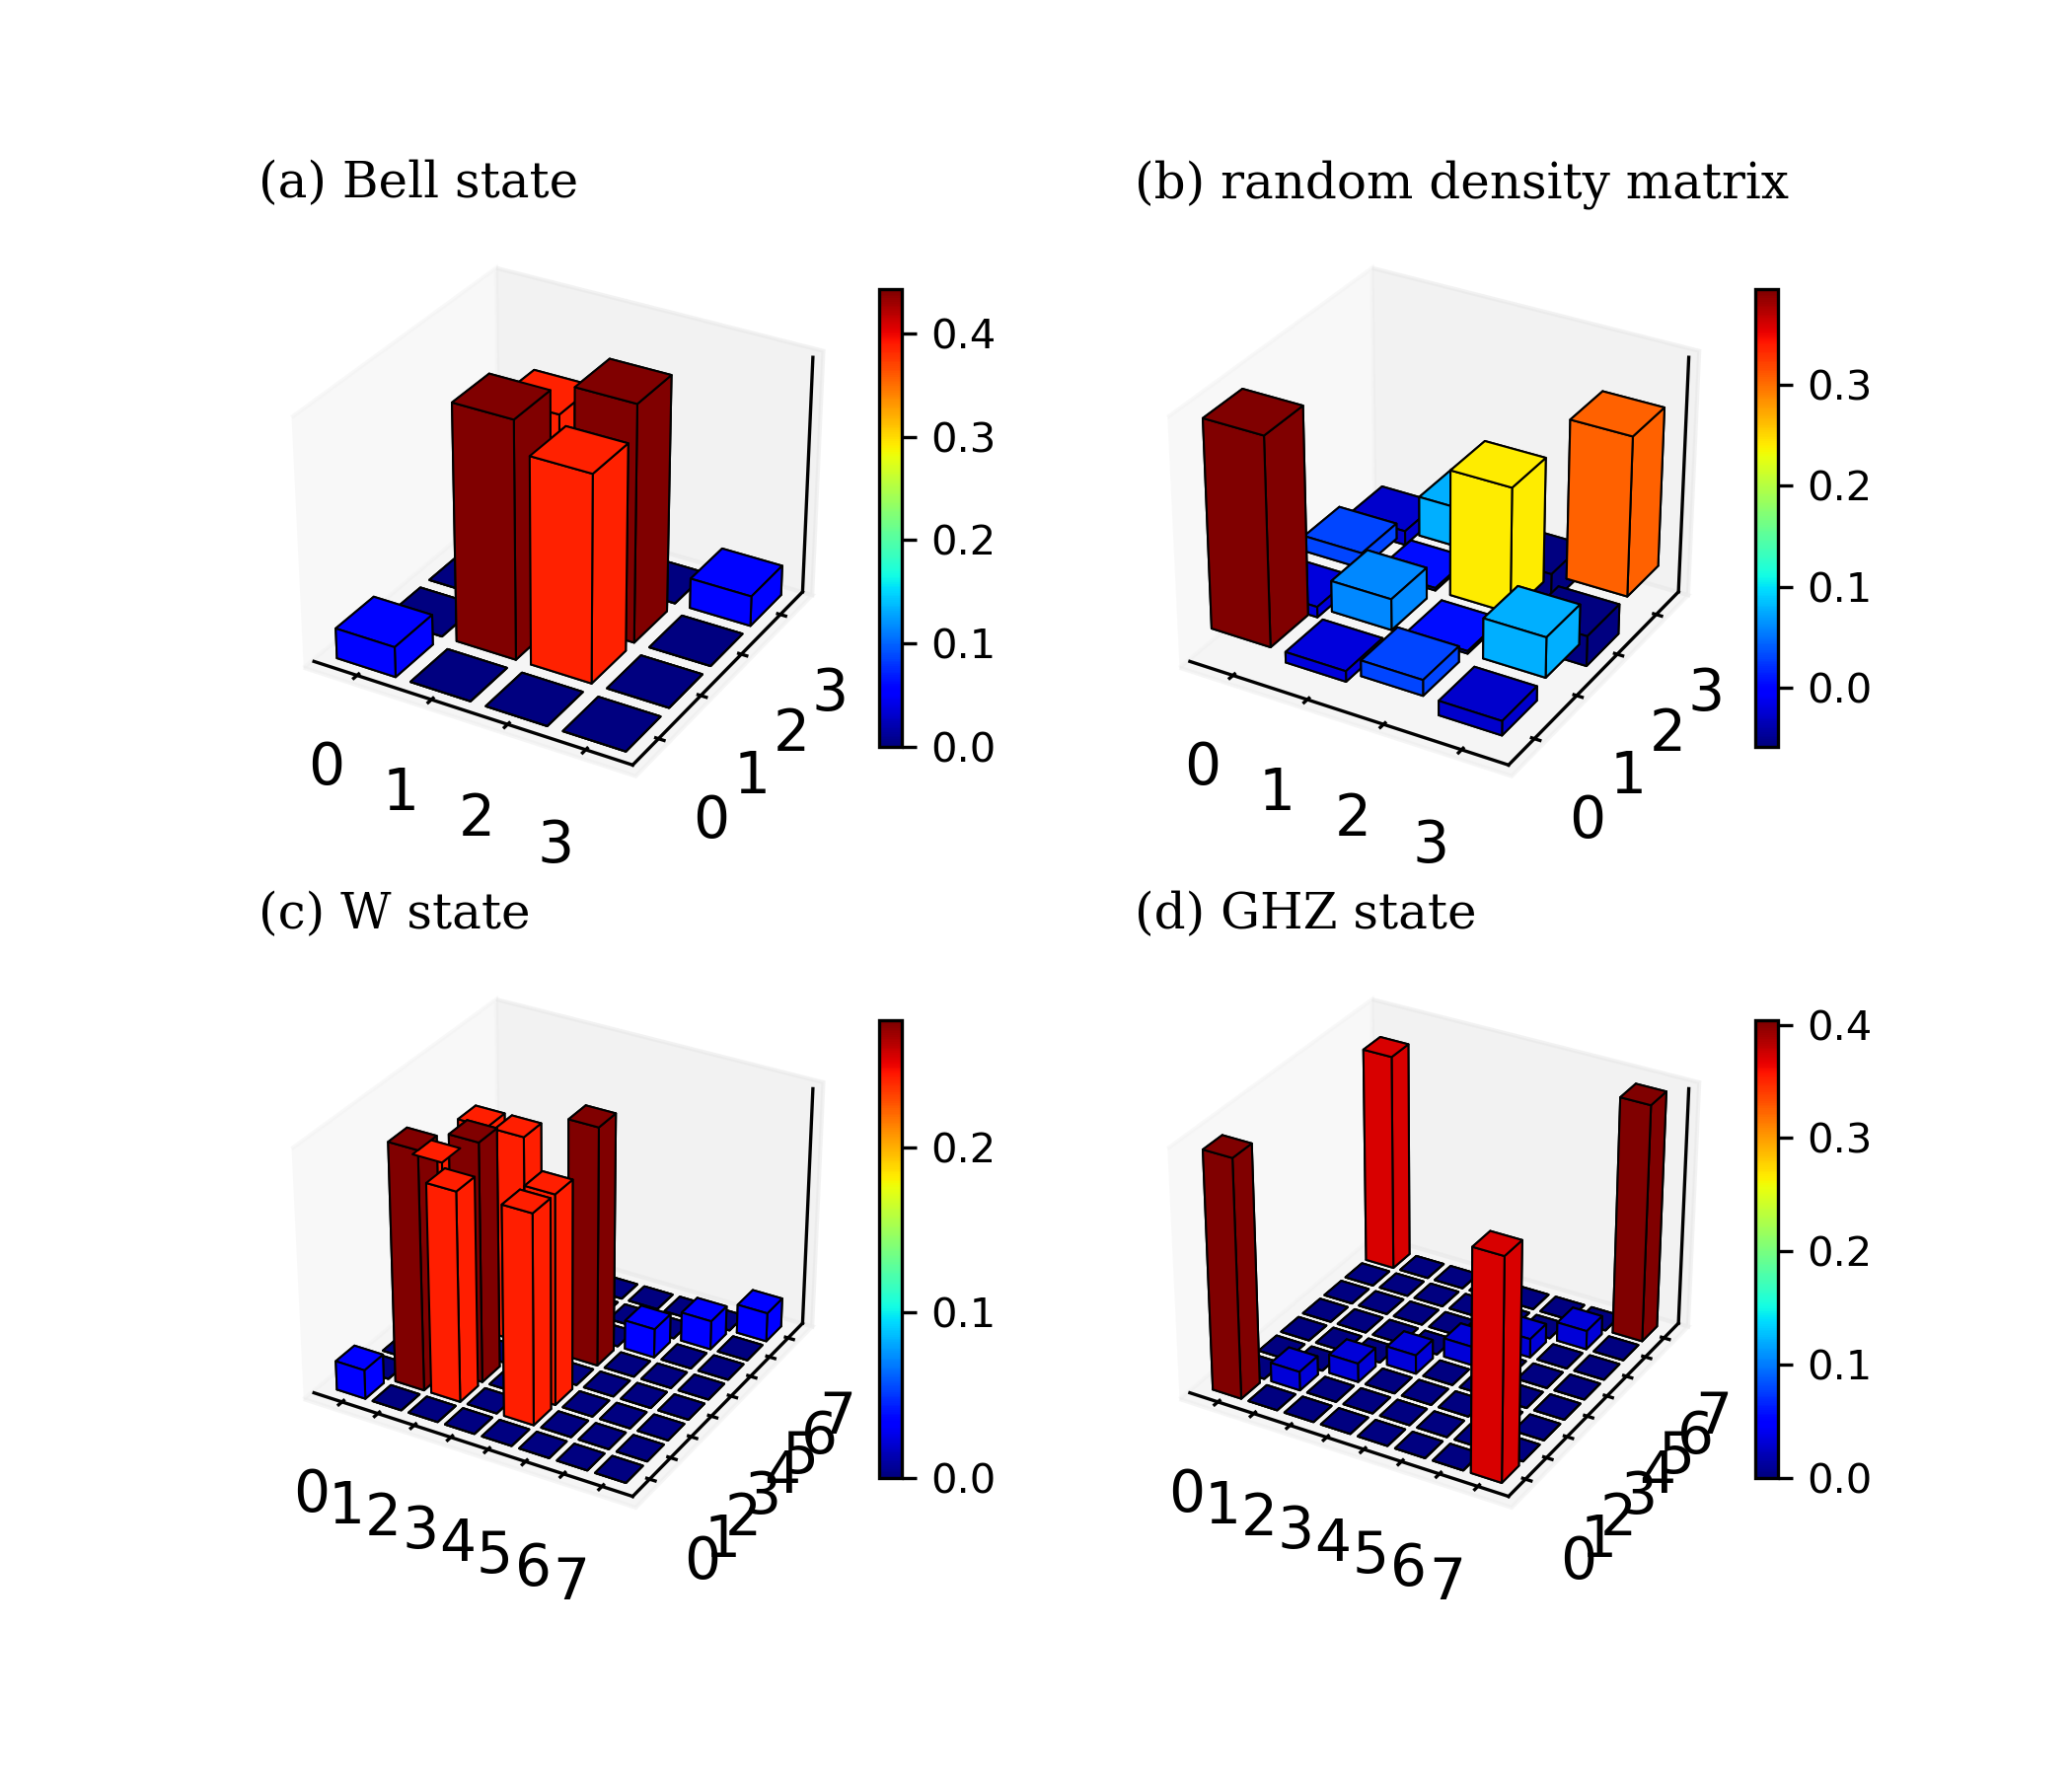
\includegraphics[width=.9\linewidth]{./Code/dataset_sample.png}
		% \caption{(a) three-qubit W state, (b) GHZ state with white noise}
	\end{subfigure}
	\begin{subfigure}{0.55\textwidth}
	\centering
		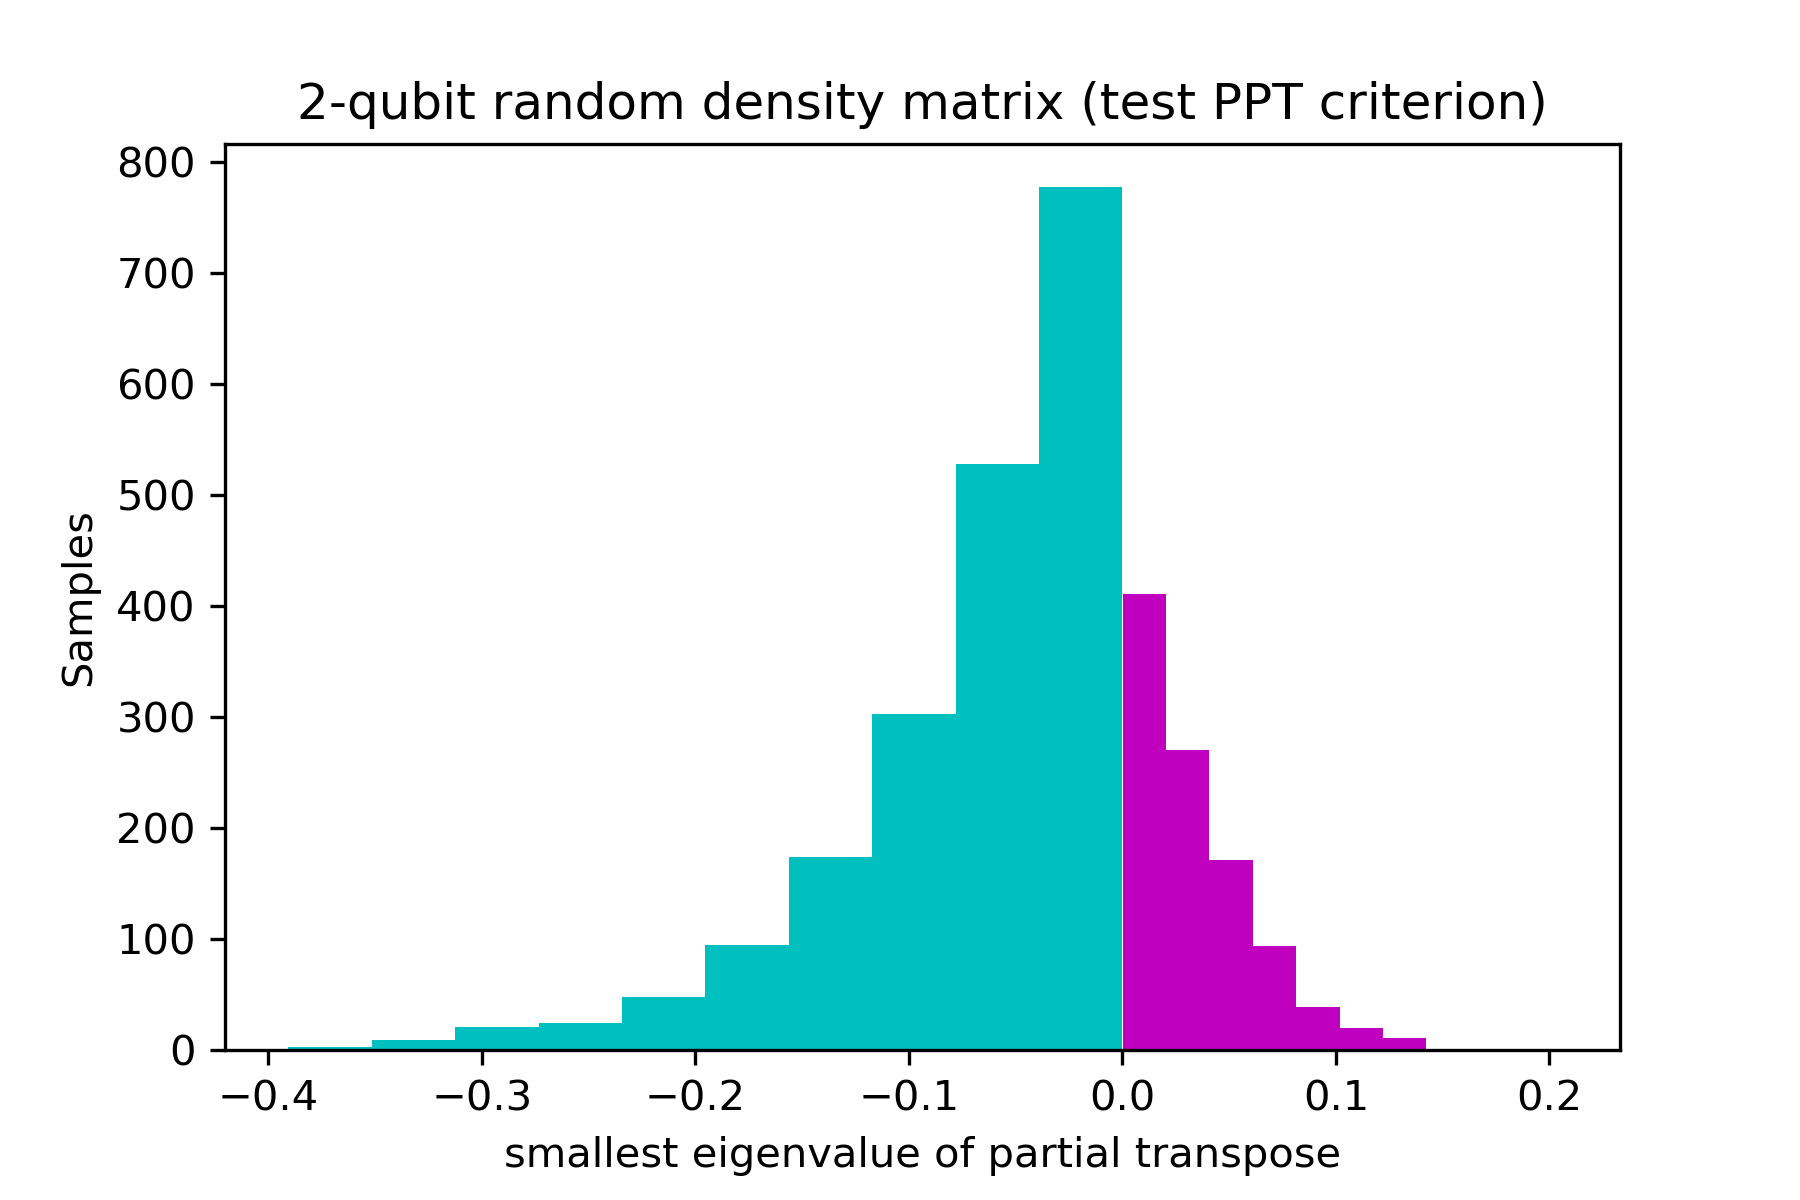
\includegraphics[width=.9\linewidth]{./Code/two_qubit_PPT_hist.png}
		% \caption{PPT criterion (2-qubit random density matrix)}
	\end{subfigure}
	\caption{data praparation: random states (a) three-qubit W state, (b) GHZ state with white noise (c) (d) (e) PPT}
\end{figure}
QuTiP library \cite{johanssonQuTiPPythonFramework2013}; quantum circuit \cite{liPulselevelNoisyQuantum2022}

entangled states generation: Bell, GHZ, W state, graph (cluster) state
\begin{equation}
	\cos(\theta) \ket{00} + \sin(\theta)e^{\ii \phi} \ket{11}
	,\;
	\cos(\theta) \ket{01} + \sin(\theta)e^{\ii \phi} \ket{10}
\end{equation}

separable states generation
\begin{itemize}
	\item 2-qubit: bipartite
	\item Training data for $\dm_b^{(1,2,3)}$ generated by sampling over the Hilbert-Schmidt-distributed space of single-qubit and bi-qubit density matrices. As for the entangled state, we again use the Werner state to generate the training data for that class of states.
	\begin{equation}
		\dm_{A|B|C},\;
		\dm_{A|BC},\;
		\dm_{AB|C},\;
		\dm_{B|AC}
		\quad
	% \end{equation}
	% \begin{equation}
		\ket{rand}_A \otimes \ket{rand}_B,\;
		\ket{rand}_A \otimes \ket{entangle}_{BC},\;
	\end{equation}
\end{itemize}
% \begin{figure}[!ht]
% 	\centering
% 	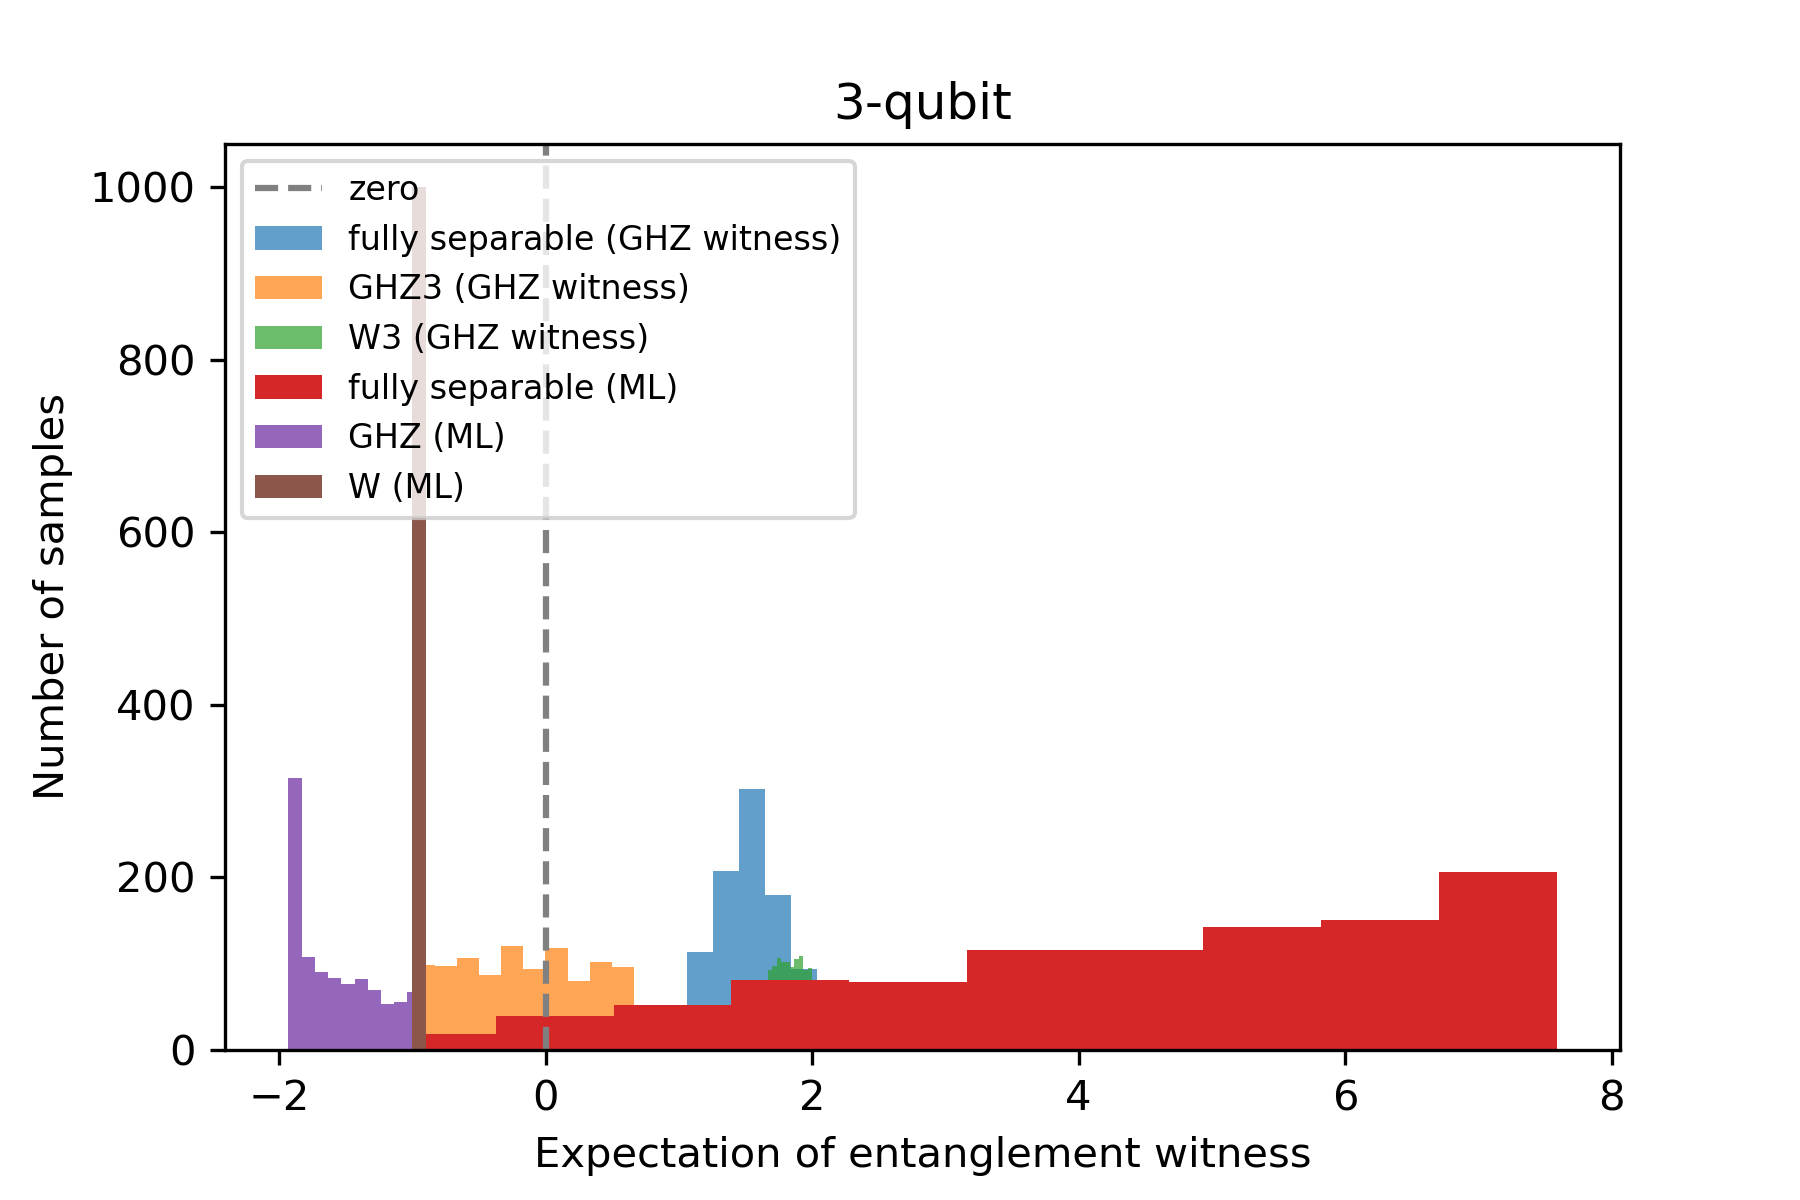
\includegraphics[width=.5\linewidth]{./notebook/three_qubit_hist.png}
% 	% 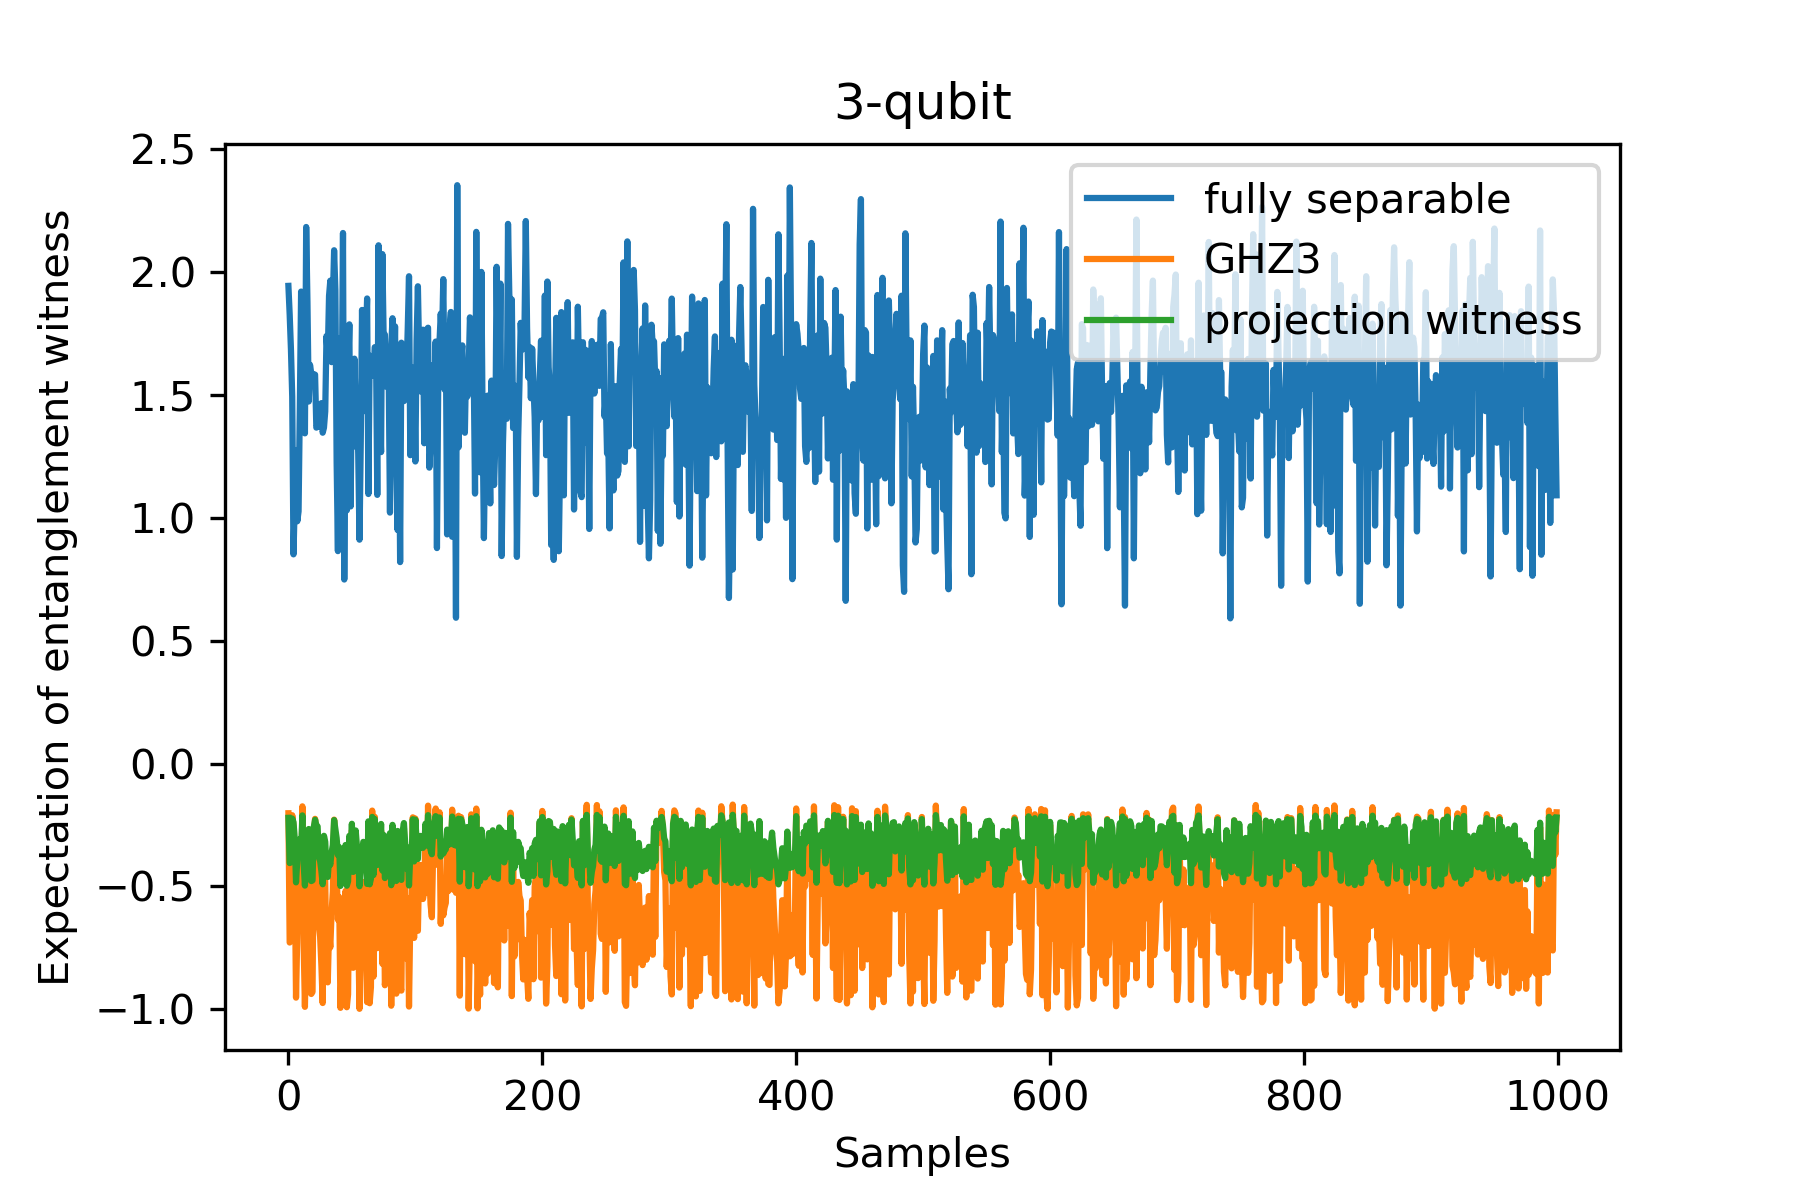
\includegraphics[width=.5\linewidth]{three_qubit.png}
% 	\caption{Compare different entanglement witnesses: GHZ, fully separable}
% \end{figure}

\subsection{Classification accuracy and comparison}
\subsubsection{Hyperparameters and settings}
We consider a set of different regularization parameters,...

The goal of RFE is to eliminate non-essential features by recursively considering smaller and smaller subsets of the original features using a greedy algorithm. Initially, RFE takes the SVM we trained and ranks the coefficients by their magnitudes, with the lowest one pruned away; then the model is trained again with the remaining features.
\begin{figure}[!ht]
	\centering
	\begin{subfigure}{0.49\textwidth}
	\centering
		\includegraphics[width=.9\linewidth]{./Code/feature_space_2.png}
		% \caption{two-dimensional embedding: feature space, recursive feature elimination}
	\end{subfigure}
	\begin{subfigure}{0.49\textwidth}
	\centering
		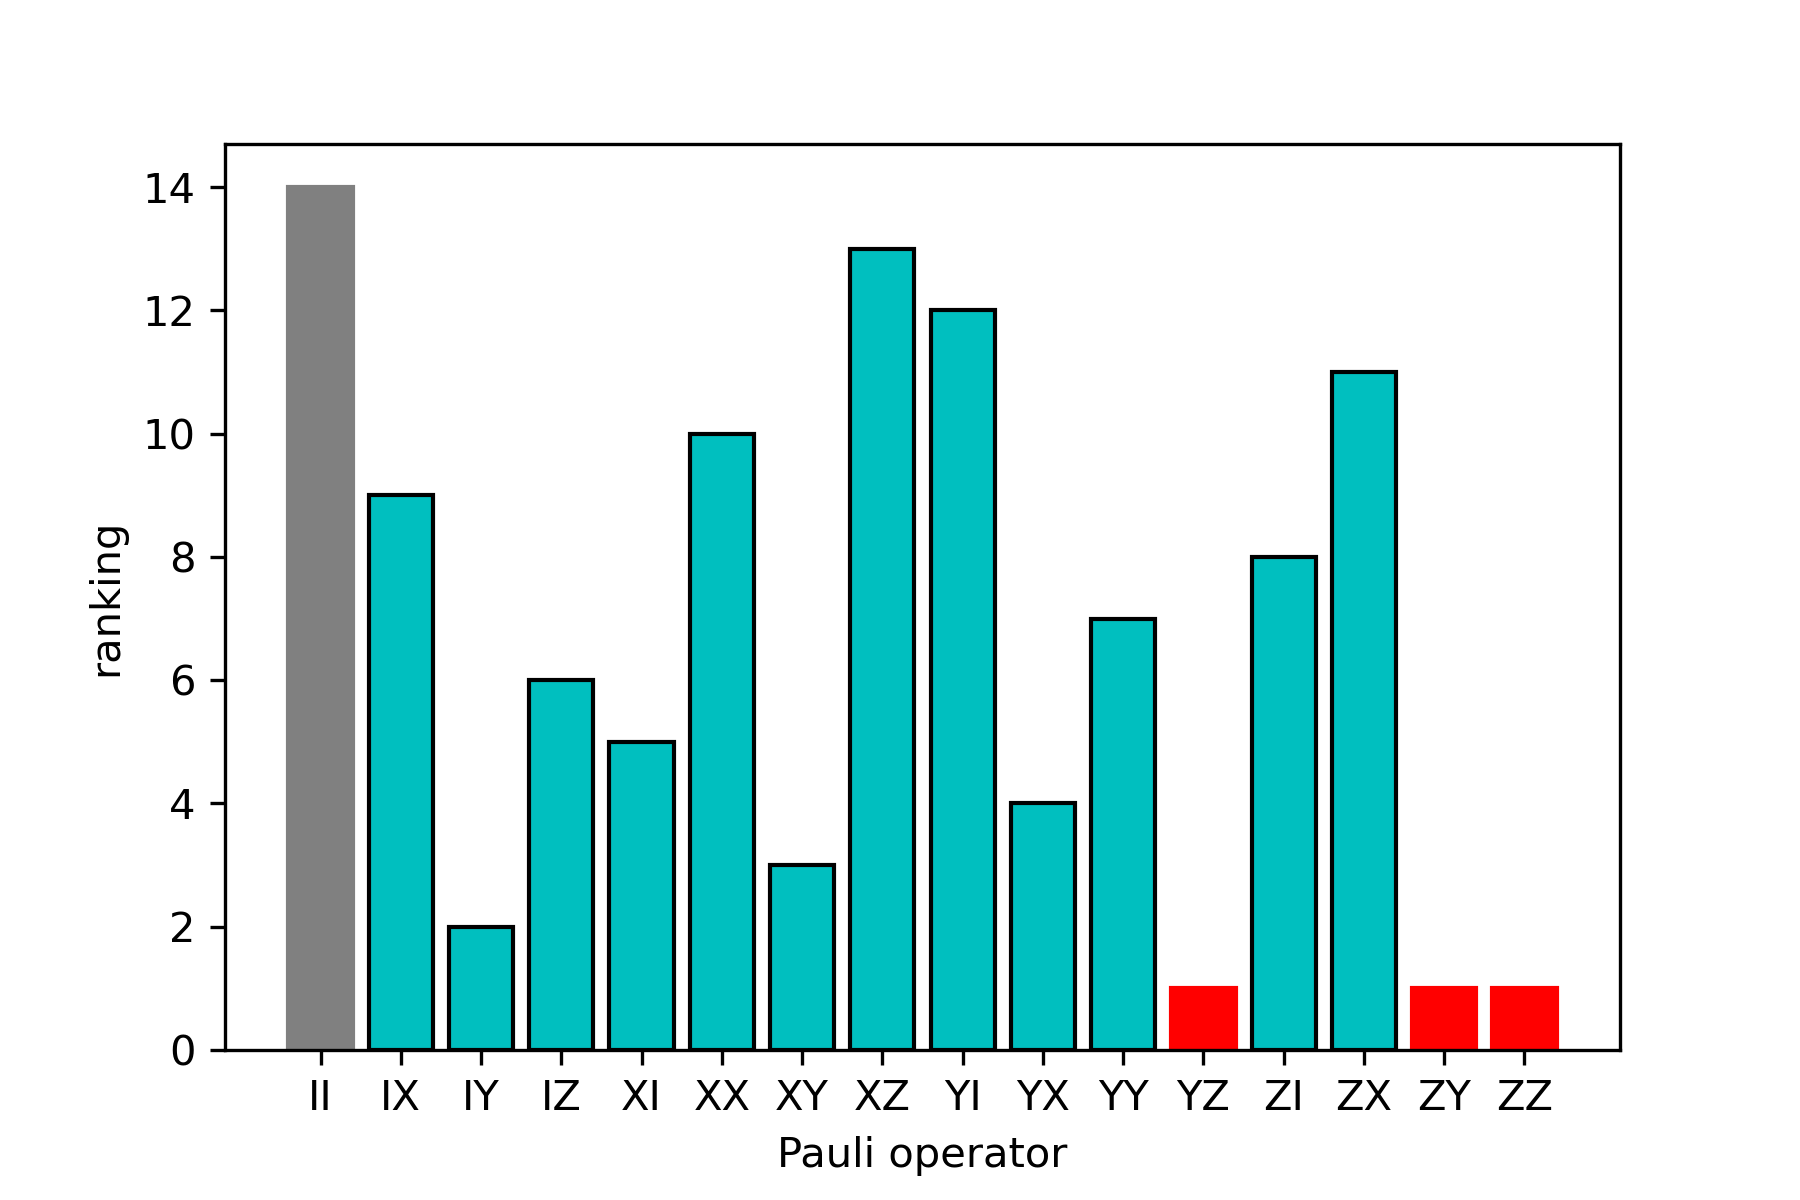
\includegraphics[width=.9\linewidth]{./Code/feature_rank.png}
		% \caption{feature ranking}
	\end{subfigure}
	\caption{(a) two-dimensional embedding: feature space, recursive feature elimination; (b) feature ranking}
\end{figure}
% \begin{figure}[!ht]
% 	\centering
% 	\includegraphics[width=.4\linewidth]{./notebook/feature_space_2.png}
% 	\caption{feature space, recursive feature elimination}
% \end{figure}
\begin{figure}[!ht]
	\centering
	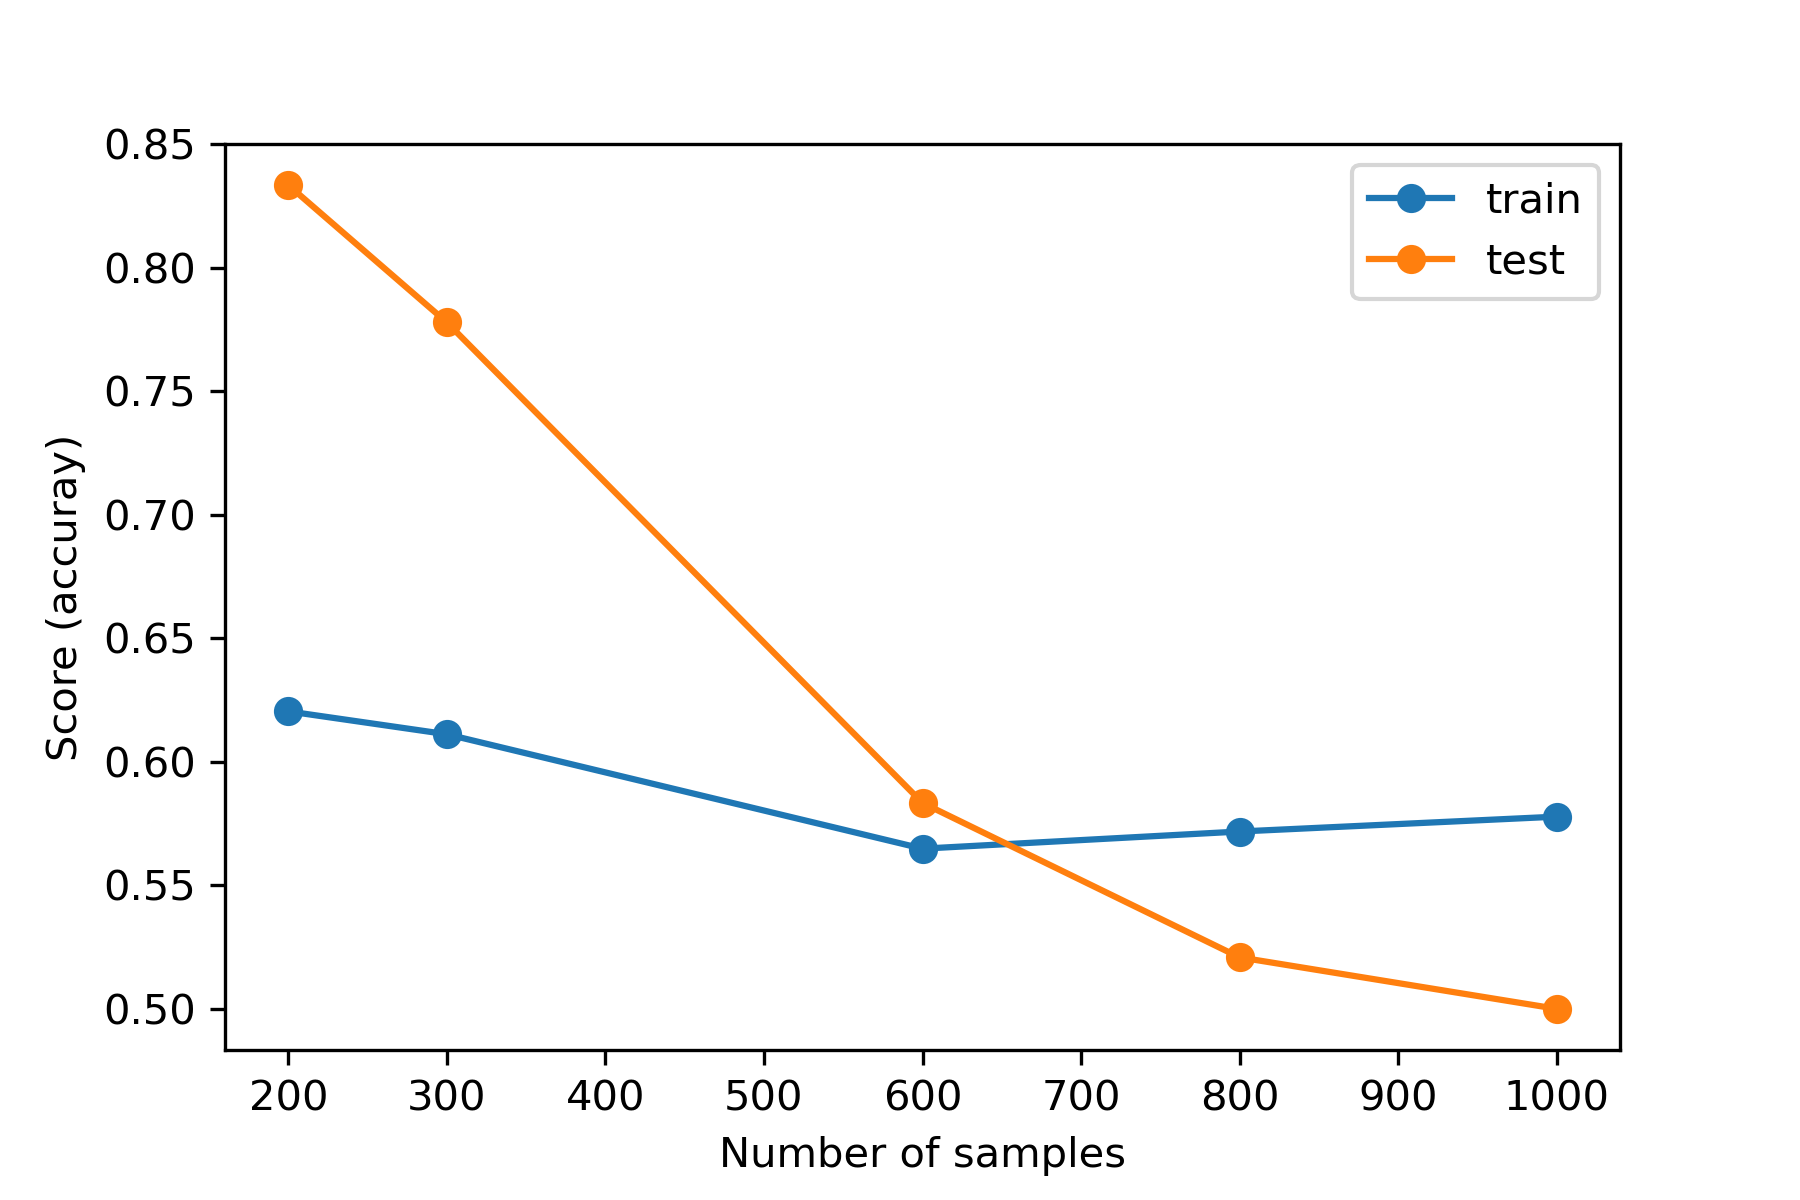
\includegraphics[width=.4\linewidth]{./Code/two_qubit_scores.png}
	\caption{accuracies (variance) VS different data sizes}
\end{figure}
\begin{figure}[!ht]
	\centering
	% \includegraphics[width=1\linewidth]{.pdf}
	\caption{number of features VS number of qubits (n). feature elimination}
\end{figure}

% \begin{figure}[!ht]
% 	\centering
% 	% \includegraphics[width=1\linewidth]{.pdf}
% 	\caption{unfaithfull; non-stabilizer}
% \end{figure}

\subsubsection{Results, feature elimination}
performance of different methods: 
% \begin{figure}[!ht]
% 	\centering
% 	\includegraphics[width=.9\linewidth]{./notebook/fidelity_witness_compare.png}
% 	% 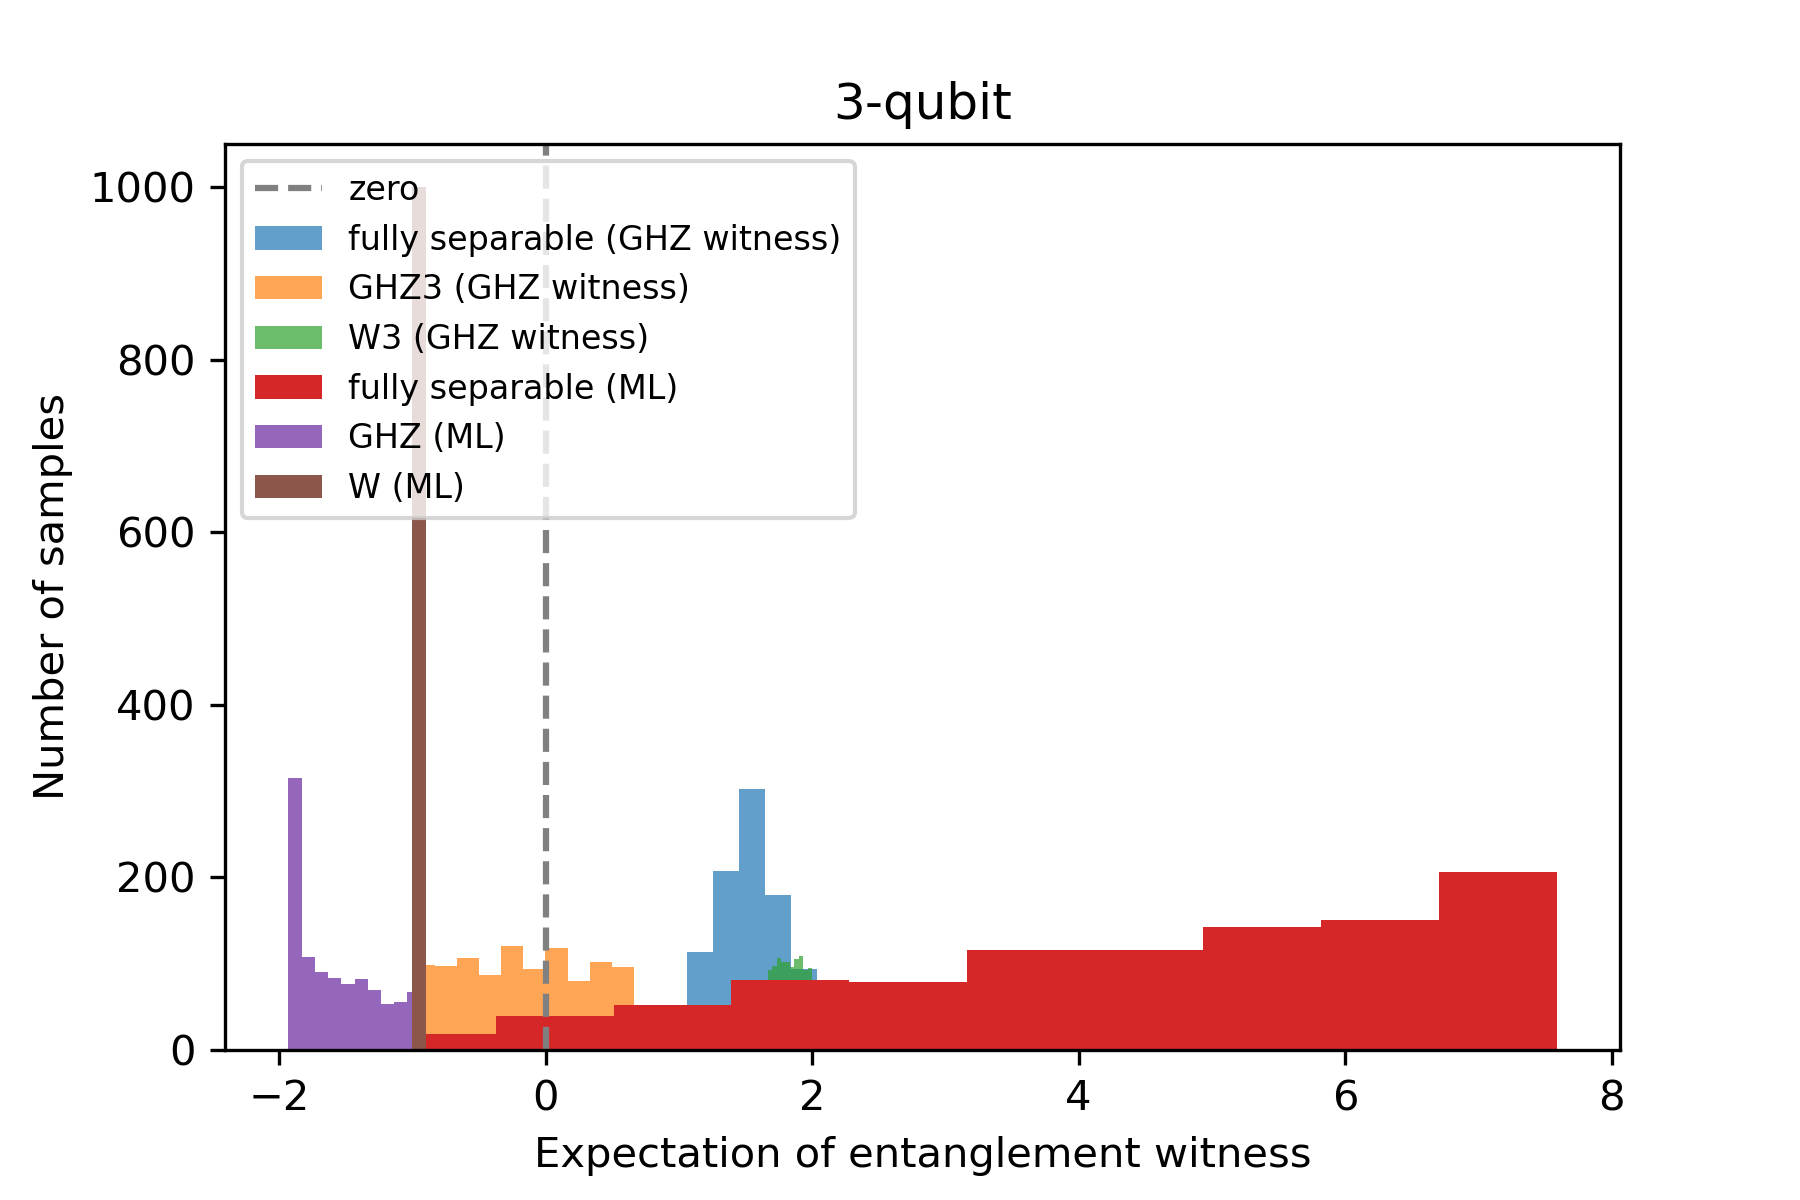
\includegraphics[width=.9\linewidth]{./notebook/three_qubit_hist.png}
% 	\caption{compare different methods: Bell inequality, witness, ML ansatz; different white noise limit, unfaithful state}
% \end{figure}
% \cite{huangPredictingManyProperties2020}
for any state $\dm_s$ with only bipartite entanglement, $\Tr(\ob \dm_s)\le 0.5$, 
while for any state $\dm_s$ with at most $W$-type entanglement, $\Tr(\ob \dm_s)\le 0.75$.
Therefore verifying that $\Tr(\ob \dm)\ge 0.5$ certifies that $\dm$ has tripartite entanglement, while $\Tr(\ob \dm)> 0.75$ certifies that $\dm$ has $\ghz$-type entanglement. \cite{acinClassificationMixedThreequbit2001}
\begin{figure}[!ht]
	\centering
	\begin{subfigure}{0.45\textwidth}
	\centering
		% \includegraphics[width=.9\linewidth]{.pdf}
		\includegraphics[width=.98\linewidth]{./Code/fidelity_witness_compare.png}
		% 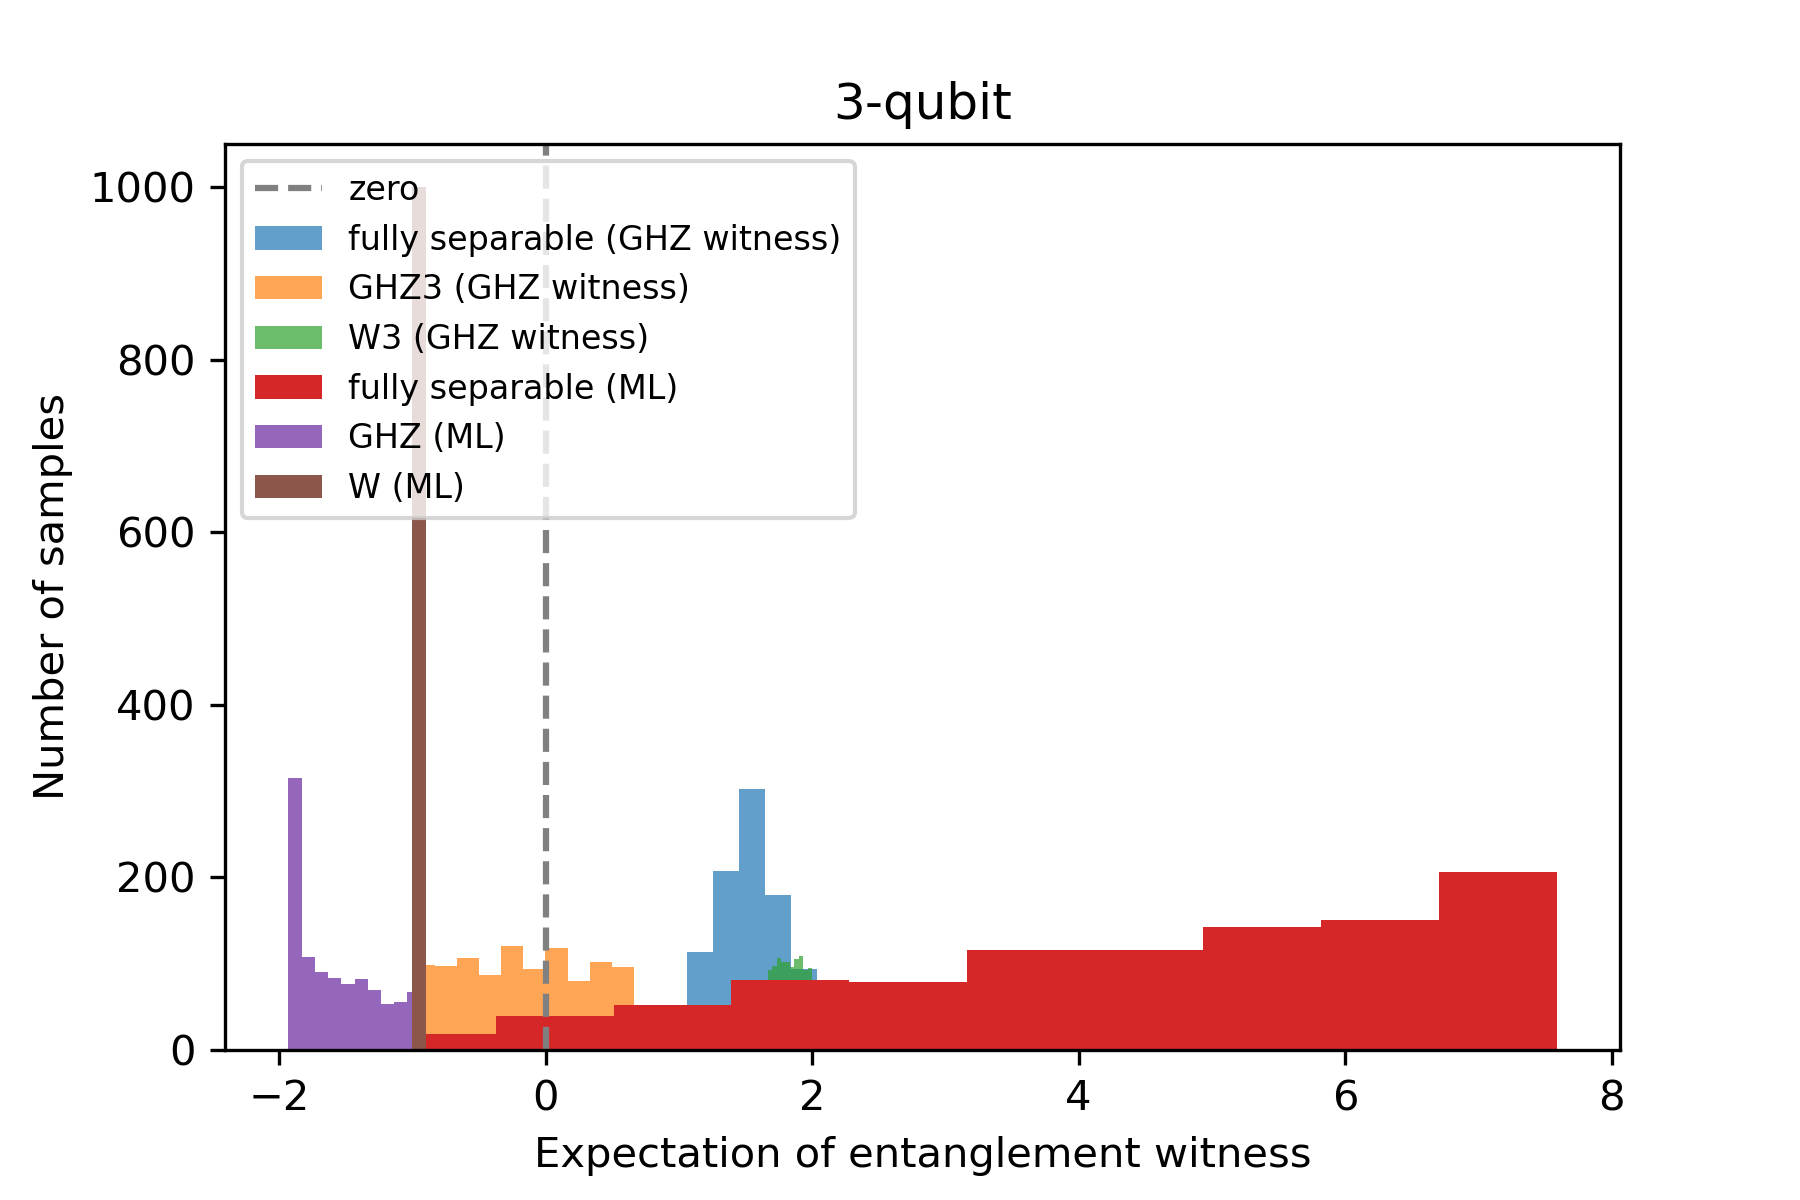
\includegraphics[width=.9\linewidth]{./notebook/three_qubit_hist.png}
		% \caption{compare different methods: Bell inequality, witness, ML ansatz; different white noise limit, unfaithful state}
	\end{subfigure}
	\begin{subfigure}{0.52\textwidth}
	\centering
		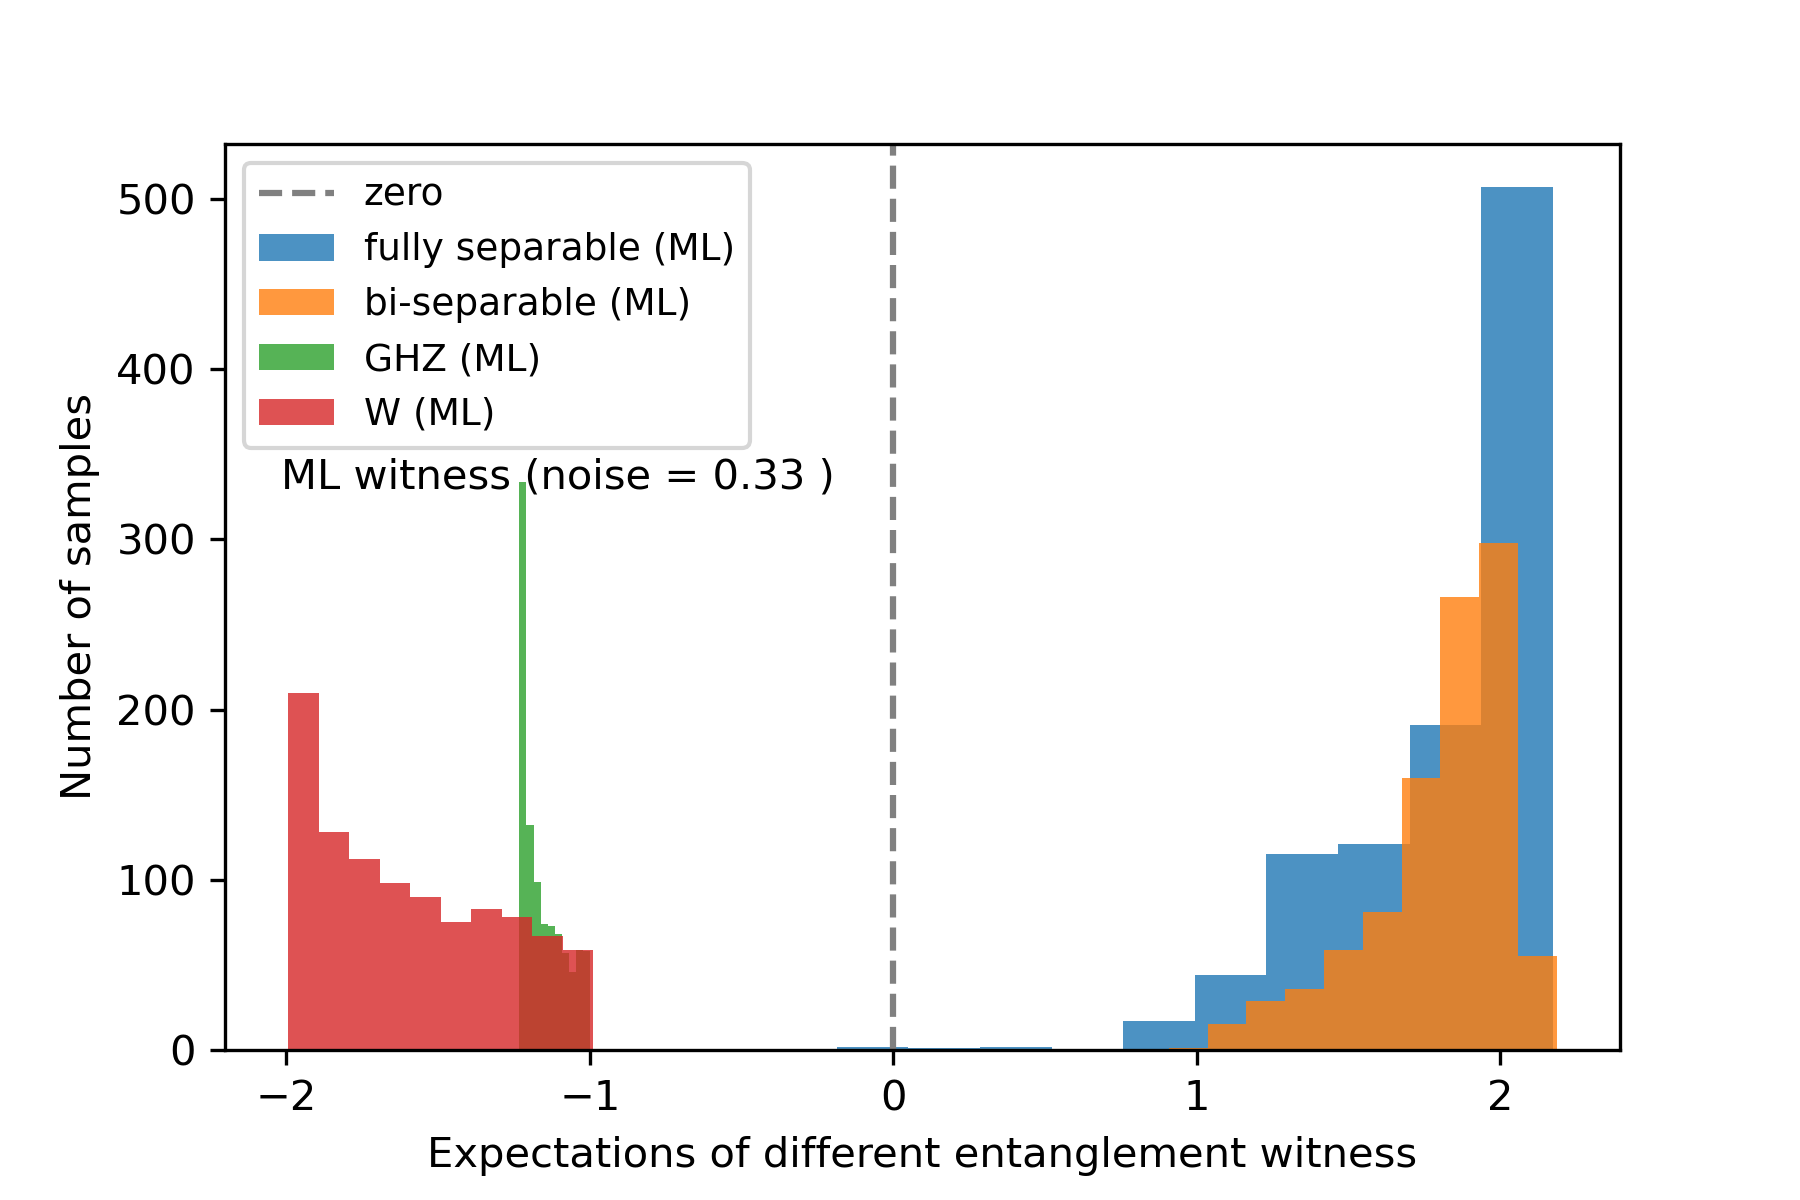
\includegraphics[width=.95\linewidth]{./Code/three_qubit_hist_.png}
		% \caption{ML witness, unfaithful}
	\end{subfigure}
	\caption{(a) compare different methods: Bell inequality, witness, ML ansatz; different white noise limit, unfaithful state; (b) ML witness for unfaithful (large white noise), non-stabilizer (W) state}
\end{figure}
% \begin{itemize}
% 	\item shadow tomography: 
% 	\item entanglement witness (no machine learning); 
% 	\item classical machine learning; 
% 	\item quantum machine learning
% \end{itemize}

% \subsection{Robustness to noise}
% tradeoff between (white noise) tolerance (robustness) and efficiency (number of measurements).

% \begin{figure}[!ht]
% 	\centering
% 	% \includegraphics[width=1\linewidth]{.pdf}
% 	\caption{robustness: accuracy VS p noise }
% \end{figure}


\section{Experiments}\label{sec:experiments}
% \subsection{Experiments}
future: experimental (photonic) implementation with a few qubits (generation, verification) \cite{luEntanglementStructureEntanglement2018}.
fully entangled graph state (ring of 16 qubits) IBM by measuring negativity \cite{wang16qubitIBMUniversal2018}
optical lattice \cite{zhouSchemeCreateVerify2022} (homogeneous, restricted measurement, different noise channels; detect GME, full entanglement).
classical shadow experiments \cite{zhangExperimentalQuantumState2021}
\cite{elbenMixedstateEntanglementLocal2020}
% \cite{zhuFlexibleLearningQuantum2022}

\section{Conclusion and discussion}
% \begin{itemize}
% 	\item experiment (generation, verification) \cite{luEntanglementStructureEntanglement2018}
% 	\item error correction? not benchmark
% \end{itemize}

\subsection*{Acknowledgements}
% \thanks{The author thanks} 
% The author thanks
% TikZiT, QuTip

%\begin{appendices}
    %\chapter{}
%\end{appendices}

% %%%%%%%%%%%%%%%Reference%%%%%%%%%%%%%%%
% % \newpage
% % \printbibliography
\bibliographystyle{apsrev4-2}
%\bibliographystyle{alpha}
\bibliography{ref}

%\begin{widetext}
\onecolumngrid
\appendix

% !TEX root = ./ew.tex


\section{Definitions}\label{sec:definitions}
\begin{definition}[density matrix]\label{def:density_matrix}
	pure state $\ket{\psi}$;
	A quantum state $\dm$ is defined to be a positive operator $ \dm \in \text{End}(V )$ with $\Tr( \dm ) = 1$.
	density matrix $\dm$ (trace one, Hermitian, PSD)...
\end{definition}
\begin{definition}[POVM]\label{def:povm}
	A positive-operator valued measurement (POVM) $M$ consists of a set of positive operators that sum to the identity operator $\identity$. 
	When a measurement $M = \qty{ E_1 , \dots , E_k }$ is applied to a quantum state $\dm$, the outcome is $i \in [k]$ with probability $p_i = \tr( \dm E_i )$.
	observables ... $\expectation[x]\equiv\expval{\ob_x}:=\tr(\ob_x\dm)$
\end{definition}
\begin{definition}[positive, semidefinite]\label{def:psd}
	denoted $X \preceq Y $ provided $Y-X $ is positive
\end{definition}
\begin{definition}[partial trace]\label{def:partial_trace}
	% partial trace;
	reduced density matrix $\dm_A = \Tr_B(\dm_{AB})$
\end{definition}
% \begin{definition}[partial trace]
% 	partial trace
% \end{definition}
\begin{definition}[partial transpose]\label{def:partial_transpose}
	\cite{horodeckiSeparabilityMixedStates1996}
	The partial transpose (PT) operation - acting on subsystem $A$ - is defined as
	\begin{equation}
		\op{k_A,k_B}{l_A,l_B}^{\T_A}
		:= \op{l_A,k_B}{k_A,l_B}
	\end{equation}
	where $\qty{\ket{k_A,k_B}}$ is a product basis of the joint system AB.
\end{definition}
\begin{definition}[maximally entangled]
	a state vector is \emph{maximually entangled} $\iff$ the reduced state at one qubit is maximally mixed, i.e.,
	$\Tr_A(\op{\psi})=\frac{1}{2}$.
\end{definition}
\begin{definition}[entropy]\label{def:entropy}
	In quantum mechanics (information), the von Neumann \emph{entropy} of a density matrix is $H_N(\dm): = -\Tr(\dm \log \dm)=-\sum_i\lambda_i\log(\lambda_i)$;
	In classical information (statistical) theory, the Shannon entropy of a probability distribution $P$ is  $H_S(P):= -\sum_i P(x_i) \log P(x_i)$.
	relative entropy (\nameref{def:divergence})
\end{definition}
\begin{definition}[entanglement entropy]\label{def:entanglement_entropy}
	The bipartite \emph{von Neumann entanglement entropy} $S$
	is defined as the von Neumann entropy of either of
	its reduced density matrix $\dm_A$.
	For a pure state $\dm_{AB}=\op{\Psi}{\Psi}_{AB}$,
	it is given by
	\begin{equation}
		E(\Psi_{AB}) 
		= S(\dm_A)
		= -\Tr(\dm_A \log \dm_A)
		= -\Tr(\dm_B \log \dm_B)
		= S(\dm_B)
	\end{equation}
	where $\dm_A= \Tr_B(\dm_{AB})$ and $\dm_B = \Tr_A(\dm_{AB})$ 
	are the reduced density matrices for each partition.
	With Schmidt decomposition (\cref{eq:schmidt_decomposition}), the entropy of entanglement is simply $-\sum_ip_i^2\log(p_i)$.
	the $n$th Renyi entropy,
	$S_n = \frac{1}{n-1} \log (R_n)$
	% \begin{equation}
	% 	S_n = \frac{1}{n-1} \log (R_n)
	% \end{equation}
	where $R_n = \Tr(\dm^n_A)$
\end{definition}


% \subsubsection{Distance measures}\label{sec:distance_measure}
\begin{definition}[fidelity]\label{def:fidelity}
	Given a pair of states (target $\dm$ and prepared $\dm'$), 
	Uhlmann fidelity $F(\dm,\dm') : = \Tr(\sqrt{\sqrt{\dm}\dm'\sqrt{\dm}})\equiv\norm{\sqrt{\dm}\sqrt{\dm'}}_1$, where $\sqrt{\dm}$ dentoes the positive semidefinite square root of the operator $\dm$. (infidelity $1-F(\dm,\dm')$)
	For any mixed state $\rho$ and pure state $\ket{\psi}$, $F(\dm,\op{\psi})=\sqrt{\mel{\psi}{\dm}{\psi}}\equiv \sqrt{\Tr(\dm\op{\psi})}$ which can be obtained by the Swap-test[?].
	linear fidelity or overlap $F(\dm,\dm'):=\tr(\dm\dm')$.
	% \begin{equation}
	% 	F(\ket{\psi},\ket{\psi'}) :=
	% \end{equation}
	% \begin{equation}
	% 	F(\rho,\rho') : = \Tr \sqrt{\sqrt{\rho}\rho'\sqrt{\rho}}
	% \end{equation}
\end{definition}
different distance measures \cite{badescuQuantumStateCertification2017}
\begin{definition}[norm]\label{def:norm}
	Schatten p-norm $\norm{x}_p:= (\sum_i \abs{x_i}^p)^{1/p}$.
	Euclidean norm $l_2$ norm;
	Spectral (operator) norm $\norm{\vbx}_{\infty}$;
	Trace norm $\norm{A}_{\Tr}\equiv\norm{A}_{1}:=\Tr(\abs{A})\equiv\Tr(\sqrt{A^\dagger A})$, $\abs{A}:=\sqrt{A^\dagger A}$, $p=1$;
	Frobenius norm $\norm{A}_{F}:=\sqrt{\Tr(A^\dagger A)}$, $p=2$;
	Hilbert-Schmidt norm $\norm{A}_{HS}:=\sqrt{\sum_{i,j} A_{ij}^2 }=?\sum_{i\in I}\norm{Ae_i}_H^2$;
	Hilbert-Schmidt inner product $\expval{A,B}_{\textup{HS}}:=\Tr(A^\dagger B)$,
	Frobenius inner product $\expval{A,B}_{\textup{F}}:=\Tr(A^\dagger B)$?
	(in finite-dimensionala Euclidean space, the HS norm is identical to the Frobenius norm)
	Although the Hilbert-Schmidt distance is arguably not too meaningful, operationally, one can use Cauchy-Schwarz to relate it to the very natural trace distance.
\end{definition}
\begin{definition}[distance]\label{def:distance}
	For mixed states, trace distance $d_{\tr}(\dm,\dm') : = \frac{1}{2} \norm{\dm-\dm'}_1$.
	For pure states, $d_{\tr}(\ket{\psi},\ket{\psi'}) : = \frac{1}{2}\norm{\op{\psi} -\op{\psi'}}_1 = \sqrt{1-\abs{\ip{\psi}{\psi'}}^2}$.
	% \begin{equation}
	% 	d_{tr}(\rho,\rho') : = \frac{1}{2} \norm{\rho-\rho'}_1
	% \end{equation}
	fidelity and trace distance are related by the inequalities
	\begin{equation}
		1-F\le D_{\tr}(\dm,\dm') \le \sqrt{1-F^2}
	\end{equation}
	variation distance of two distribution $d_{var}(p,p') : = \frac{1}{2} \sum_i \abs{p_i-p_i'} = \frac{1}{2} \norm{p-p'}_1$.
	% It also has an operational meaning: it is the greatest probability with which one can discriminate a draw from p and a draw from q.
	$l_2$ distance ... Hellinger distance ... HS distance $D_{\text{HS}}(\dm,\dm'): = \norm{\dm-\dm'}_{\text{HS}}=\sqrt{\Tr((\dm-\dm')^2)}$
	% As a probability metric, the $l_2$ distance is somewhat unnatural. For example, it does not satisfy the “data processing inequality”, meaning that there is a stochastic operation that increases $l_2$ distance. However it is by far the easiest distance to calculate, as it is a simple polynomial in p and q; further, it can be related to the total variation distance
\end{definition}


\begin{definition}[input model]\label{def:input_model}
	several common input (encoding) models in quantum algorithms: 
	\begin{itemize}
		% \item qubit (basic) encoding?: given a vector $\vb{z}\in\integer^d$, 
		% $\ket{\vb{z}}=\bigotimes_i^d \ket{\vbx_i}$ where $\vbx_i$ is the binary representation of $z_i$,
		% need $\bigO(d\cdot \log(\max(z_i)))$ (not space efficient)

		% \item phase encoding?

		\item \textbf{amplitude encoding}: given a normalized vector $\vbx\in\realnumber^d$, the quantum state $\ket{\vbx}=\sum_z^d x_z\ket{z}$. 
		need $\log(d) $ qubits for a data point; 
		In general, it is hard to prepare such state. (subject to dequantization \cite{tangQuantumPrincipalComponent2021}). 
		typical encoding method for quantum machine learning for classical problems (such as image classification).
		% qubit (basic) encoding (inefficient? space)

		\item \textbf{unitary encoding}: quantum simulation (Hamiltonian); quantum random walk (adjacency matrix); oracle (controlled) unitary, e.g., quantum phase estimation;
		\nameref{def:graph_state} encoding (discrete, efficient in space/time?, isomorphism?)

		\item \textbf{quantum data}: quantum state $\ket{\psi}$ or $\dm$ from real-world experiments or designed quantum circuits $\U$.
		no input problem? more efficient? for quantum algorithms
		(composed coherently to collect quantum data)

		% \item graph state encoding: \nameref{def:graph_state}, discrete, efficient? space (time), isomorphism?

		% \item (quantum) oracle: $\oracle \ket{i,a}=\ket{i,a+x_i}$; quantum oracle: unitary and controlled unitary
	\end{itemize}
\end{definition}


% \subsection{Stabilizer formalism}\label{sec:stabilizer_formalism}
denote a group by $\group$ and a subgroup $\subgroup$. 
\begin{definition}[Pauli group]
\end{definition}
\begin{definition}[Clifford group]\label{def:clifford}
\end{definition}
\begin{definition}[Stabilizer]\label{def:stabilizer}
	An observable $S_k$ is a stabilizing operator of an $n$-qubit state $\ket{\psi}$ if the state $\ket{\psi}$ is an eigenstate of $S_k$ with eigenvalue 1,

	A stabilizer set $S = \qty{ S_1, \dots , S_n}$ consisting of n mutually commuting and independent stabilizer operators is called the set of stabilizer “generators”.
\end{definition}
Many highly entangled $n$-qubit states can be uniquely defined by $n$ stabilizing operators which are locally measurable, i.e., they are products of Pauli matrices.
A stabilizer $S_i$ is an n-fold tensor product of $n$ operators chosen from the one qubit Pauli operators $\qty{\identity,X,Y,Z}$.

\section{Machine learning background}
% As these areas are extremely broad, we cannot completely review all known literature; we will simply give pointers to some of the best known and most relevant results.

% In this work, we restrict ourself to supervised learning (mainly SVM), where we are given a set of labeled data for training to predict labels of new data.

Notations:
The (classical) training data (for supervised learning) is a set of $m$ data points $\qty{(\vbx^{(i)}, y^{(i)})}^{m}_{i=1}$ 
where each data point is a pair $(\vbx,y)$.
Normally, the input (e.g., an image) $\vbx:= (x_1,x_2,\dots,x_d) \in \realnumber^d$  is a vector where $d$ is the number of \emph{features}
and its \emph{label} $y\in\Sigma$ is a scalar with some discrete set $\Sigma$ of alphabet/categories. 
For simplicity and the purpose of this paper, we assume $\Sigma=\qty{-1,1}$ (binary classification).


\subsection{Support vector machine}\label{sec:svm}
SVM is a typical supervised learning algorithm for classification. Taking the example of classifying cat/dog images, supervised learning means we are given a dataset in which every image is labeled either a cat or a dog such that we can find a function classifying new images with high accuracy. More precisely,  the training dataset is a set of pairs of features X and their labels y. In the image classification case, features are obtained by transforming all pixels of an image into a vector. In SVM, we want to find a linear function, that is a hyperplane which separates cat data from dog data. So, the prediction label is given by the sign of the inner product (projection) of the hyperplane and the feature vector. We can observe that the problem setting of image classification by SVM is quite analogous to entanglement detection, where input data are quantum states now and the labels are either entangled or separable.


\begin{definition}[SVM]\label{def:svm}
	Given a set of (binary) labeled data,
	support vector machine (SVM) is designed to
	find a hyperplane (a linear function) such that maximize the margin between two partitions...
	\begin{equation}
		\max_{\vb{w}} 
		....
	\end{equation}
\end{definition}

\subsubsection{kernel method}
However, note that SVM is only a linear classifier. while most real-world data, such as cat/dog images and entangled/separable quantum states are not linearly separable. For example, with this two dimension dataset, we are unable to find a hyperplane to separate red points from the purple points very well. Fortunately, there is a very useful tool called kernel method or kernel trick to remedy this drawback. The main idea is mapping the features to a higher dimensional space such that  they can be linearly separated in the high dimensional feature space. Just like this example, two dimensional data are mapped to the three dimensional space. Now, we can easily find the separating plane. With SVM and kernel methods, we expect to find a generic and flexible way for entanglement detection.
\nameref{def:kernel}
\begin{definition}[kernel]\label{def:kernel}
	In general, the kernel function $\kernel:\mathcal{X}\times \mathcal{X} \to \realnumber$ measures the similarity between two input data points by an inner product
	\begin{equation}
		\kernel (\vbx,\vbx') : = \expval{\phi(\vbx),\phi(\vbx')}
	\end{equation}
	If the input $\vbx\in \realnumber^d$ (conventional machine learning task, e.g., image classification), the feature map $\phi(\vbx): \realnumber^d\to \realnumber^n$ ($d < n$) from a low dimensional space to a higher dimensional space.
	The corresponding kernel (Gram) matrix $\mathbf{K}$ should be a positive, semidefinite (PSD) matrix, i.e. all eigenvalues are non-negative
\end{definition}
\begin{example}[kernels]
	Some common kernels: 
	the polynomial kernel $\kernel_{\text{poly}}(\vbx,\vbx') := (1+\vbx\cdot\vbx')^q$ with feature map $\phi(\vbx)$ ...
	The Gaussian kernel
	$\kernel_{\text{gaus}}(\vbx,\vbx') := \exp(-\gamma\norm{\vbx-\vbx'}^2_2)$ 
		% \begin{equation}
		% 	\kernel_{\text{gaus}}(\vbx,\vbx') := \exp(-\norm{\vbx-\vbx'}^2/(2\beta))
		% \end{equation}
	with an infinite dimensional feature map $\phi(\vbx)$.
	An important feature of kernel method is that kernels can be computed efficiently without evaluating feature map (might be infinite dimension) explicitly.
	% \begin{itemize}
	% 	\item \emph{Gaussian kernel}; 
	% 	\begin{equation}
	% 		\kernel_{\text{gaus}}(\vbx,\vbx') := \exp(-\norm{\vbx-\vbx'}^2/(2\beta))
	% 	\end{equation}
	% 	note that infinite dimensional feature map

		% \item \emph{graph kernel} \cite{kriegeSurveyGraphKernels2020}: given a pair of graphs $(\graph,\graph')$
		% \begin{equation}
		% 	\kernel (\graph,\graph')  =
		% \end{equation}
		% quantum graph kernel $\kernel (\graph,\graph')  = \abs{\ip{\graph}{\graph'}}^2$ ??
		% \cite{baiQuantumJensenShannon2015}

		% \item quantum kernel (transition amplitude / quantum propagator);
		% \begin{equation}
		% 	k_Q(\rho,\rho') := \abs{\ip{\phi(x)}{\phi(x')}}^2 =\abs{\mel{0}{\U_{\phi(x)}^\dagger \U_{\phi(x')} }{0}}^2 = \Tr(\rho\rho')
		% \end{equation}
		% with quantum feature map $\phi(x): \mathcal{X}\to \op{\phi(x)}$

		% \item \emph{shadow kernel}:
		% given two density matrices $\rho$ and $\rho'$
		% \begin{equation}
		% 	k_{\shadow}(\rho,\rho') := 
		% \end{equation}

	% 	\item neural tagent kernel \cite{jacotNeuralTangentKernel2020}: proved to be equivalent to deep neural network \cite{gaoEfficientRepresentationQuantum2017}
	% \end{itemize}
\end{example}

similarity measures? advantages? why? (isomorphism?)
\begin{definition}[divergence]\label{def:divergence}
	KL divergence (relative \nameref{def:entropy}): measure the distance (similarity) between two probability distributions:
	\begin{equation}
		\kl (P || Q) := \sum P(x) \log (P(x)/Q(x))
	\end{equation}
	symmetric version: Jensen-Shannon divergence (machine learning)
	\begin{equation}
		\jsd (P || P') := \frac{1}{2} \qty(\kl(P|| M) + \kl(P'||M))
		\equiv H_S(M)-\frac{1}{2} (H_S(P) - H_S(P') ) 
	\end{equation}
	where $M=(P+P')/2$ and Shannon \nameref{def:entropy} $H_S$.
	Analogously, quantum Jensen-Shannon divergence $D_{\qjs}$ of two density matrices can be defined...
	\begin{equation}
		D_{\qjs}(\dm||\dm'):= 
		H_V(\dm_M) - \frac{1}{2} (H_V(\dm) - H_V(\dm') ) 
	\end{equation}
	as a quantum graph kernel ($\dm$ induced by quantum random walk)
\end{definition}
\begin{definition}[geometric difference]\label{def:geometric_difference}
	\begin{equation}
		g(K^1|| k^2) = \sqrt{\norm{\sqrt{K^2} (K^1)^{-1}\sqrt{K^2}}_{\infty}}
	\end{equation}
	where $\norm{\cdot}_{\infty}$ is the spectral \nameref{def:norm}.
\end{definition}

\subsubsection{Graph kernel}
\begin{definition}[graph property]\label{def:graph_property}
	% The setting of graph property testing provides a natural class of partial graph properties.
	monotone ...
\end{definition}
\begin{example}[colorable]\label{exm:colorable}
	$k$-colorable is a graph property, i.e., allow for a coloring of the vertices with $k$ colors such that no two adjacent vertices have the same color.
	A graph is bipartite $\iff$ 2-colorable.
	other graph properties: isomorphism; vertex cover; Hamiltonian cycle ...
\end{example}
\begin{problem}[graph property test]\label{prm:graph_property_test}
	\textbf{promise}: the input graph either has a property, or is $\epsilon$-far from having the property, meaning that we must change at least an $\epsilon$ fraction of the edges to make the property hold.
\end{problem}
\begin{theorem}[bounds for graph property test]
\end{theorem}
\begin{question}
	\cite{montanaroSurveyQuantumProperty2018}
	Is there any graph property which admits an exponential quantum speed-up?
	\cite{ben-davidSymmetriesGraphProperties2020}
	depends on input model (query adjacency matrix/list)
	% quantum algorithms (bounds) for graph properties \cite{ben-davidSymmetriesGraphProperties2020}
\end{question}
Graphs is another kind of data which is fundamentally different from a real value vector because of vertex-edge relation and graph isomorphism.
So, graph kernel \cite{kriegeSurveyGraphKernels2020} need additional attention.
\begin{definition}[graph kernel]\label{def:graph_kernel}
	given a pair of graphs $(\graph,\graph')$,
	\emph{graph kernel} is $\kernel (\graph,\graph')  =$.
	% \begin{equation}
	% \end{equation}
	quantum graph kernel $\kernel (\graph,\graph')  = \abs{\ip{\graph}{\graph'}}^2$ ??
	\cite{baiQuantumJensenShannon2015}	
\end{definition}

\subsubsection{Quantum kernel}
related works:
\begin{itemize}
	\item quantum kernel method: estimate kernels by quantum algorithms (circuits)	\cite{havlicekSupervisedLearningQuantum2019}
	\cite{schuldQuantumMachineLearning2019}: for classical problem (data)

	\item rigorous and robust quantum advantage of quantum kernel method in SVM \cite{liuRigorousRobustQuantum2021}. group structured data \cite{glickCovariantQuantumKernels2021}

	\item power of data in quantum machine learning \cite{huangPowerDataQuantum2021}: input??? projected quantum kernel
\end{itemize}
\begin{definition}[quantum kernel]\label{def:quantum_kernel}
	quantum kernel 
	with quantum feature map $\phi(\vbx): \mathcal{X}\to \op{\phi(\vbx)}$
	\begin{equation}
		k_Q(\rho,\rho') := \abs{\ip{\phi(\vbx)}{\phi(\vbx')}}^2 =\abs{\mel{0}{\U_{\phi(\vbx)}^\dagger \U_{\phi(\vbx')} }{0}}^2 =? \Tr(\rho\rho') \equiv \expval{\dm,\dm'}_{\textup{HS}}
	\end{equation}
	where $\U_{\phi(\vbx)}$ is a quantum circuit or physics process that encoding an input $\vbx$.
	In quantum physics, quantum kernel is also known as transition amplitude (quantum propagator);
\end{definition}
% \begin{definition}[multivariate trace estimation]\label{def:multivariate_trace_estimation}
% 	The task of estimating quantities like 
% 	\begin{equation}
% 		\Tr(\rho_1 \cdots \rho_m)
% 		\tag{multivariate traces}
% 	\end{equation}
% 	given access to copies of the quantum states $\rho_1$  through $\rho_m$.
% \end{definition}
% is a fundamental building block in quantum information science

% power of data - 
\begin{proposition}[\cite{huangPowerDataQuantum2021}]
	If a classical algorithm without training data can compute (label) $y=f(x)=\mel{x}{\U_{\textup{QNN}}^\dagger \ob U_{\textup{QNN}}}{x}$ (with amplitude encoding) efficiently (poly time in ...) for any $\U_{\textup{QNN}}$ and $\ob$, then $\nameref{def:bpp}=\nameref{def:bqp}$ (which is believed unlikely).
\end{proposition}
\begin{proposition}[\cite{huangPowerDataQuantum2021}]
	Training an arbitrarily deep quantum neural network $\U_{\qnn}$ with a trainable observable $\ob$ is equivalent to training a \nameref{def:quantum_kernel} method with kernel $k_{Q}(\vbx,\vbx')=\Tr(\dm(\vbx)\dm'(\vbx'))$
\end{proposition}
\begin{definition}[projected quantum kernel]\label{def:projected_quantum_kernel}
	....
\end{definition}


\subsection{Neural network}\label{sec:neural_network}
\subsubsection{neural network and kernel}
\begin{definition}[neural tagent kernel]\label{def:neural_tangent_kernel}
	neural tangent kernel \cite{jacotNeuralTangentKernel2020}: proved to be equivalent to deep neural network \cite{gaoEfficientRepresentationQuantum2017} in the limit ...
	\begin{equation}
		k_{\ntk} \qty(S_T(\dm_l),\tilde{S}_T(\dm_{l'}))
		=
		\expval{
			\phi^{(\ntk)}(S_T(\dm_l)),
			\phi^{(\ntk)}(\tilde{S}_T(\dm_l))
		}
	\end{equation}
\end{definition}



\subsubsection{quantum neural network}\label{sec:quantum_neural_network}
% \subsection{Unsupervised: PCA}

\section{Hardness assumptions}
\begin{definition}[\NP]\label{def:np}
	\NP, \NP-hard, \NP-complete
\end{definition}
\begin{definition}[\sharpP]\label{def:sharpp}
	\sharpP
\end{definition}
\begin{definition}[QMA]\label{def:qma}
	QMA
\end{definition}
\begin{definition}[\BPP]\label{def:bpp}
	\BPP
\end{definition}
\begin{definition}[\BQP]\label{def:bqp}
	\BQP
\end{definition}

%\end{widetext}

\end{document}